% Adapted from Alex Reustle's CMSC351 Course Notes

% This program is free software: you can redistribute it and/or modify
% it under the terms of the GNU General Public License as published by
% the Free Software Foundation, either version 3 of the License, or
% (at your option) any later version.

% This program is distributed in the hope that it will be useful,
% but WITHOUT ANY WARRANTY; without even the implied warranty of
% MERCHANTABILITY or FITNESS FOR A PARTICULAR PURPOSE.  See the
% GNU General Public License for more details.

% You should have received a copy of the GNU General Public License
% along with this program.  If not, see <http://www.gnu.org/licenses/>.
\documentclass[english, 10pt]{article}

\usepackage{notes}
\usepackage{gensymb}
\usepackage{inconsolata}
\usepackage[shellescape]{gmp}
\allowdisplaybreaks%
\newcommand{\thiscoursecode}{CMSC 320}
\newcommand{\thiscoursename}{Introduction to Data Science}
\newcommand{\thisprof}{Prof.\ John Dickerson}
\newcommand{\me}{Akilesh Praveen}
\newcommand{\thisterm}{Fall 2020}
\newcommand{\website}{https://cmsc320.github.io}%chktex 8
\usepackage{ifpdf}
\ifpdf%
\DeclareGraphicsRule{*}{mps}{*}{}
\fi
% \listfiles

\usepackage[utf8]{inputenc}
 
\usepackage{listings}
\lstloadlanguages{Python}
\usepackage{xcolor}
\usetikzlibrary{patterns}
\usepackage[many]{tcolorbox}
 
\definecolor{codegreen}{rgb}{0,0.6,0}
\definecolor{codegray}{rgb}{0.5,0.5,0.5}
\definecolor{codepurple}{rgb}{0.58,0,0.82}
\definecolor{backcolour}{rgb}{0.95,0.95,0.94}
\definecolor{codered}{rgb}{0.5,0.15,0.15}
\definecolor{commentred}{rgb}{1,0.01,0.02}
 
\lstdefinestyle{mystyle}{
    backgroundcolor=\color{backcolour},   
    commentstyle=\color{codegreen},
    keywordstyle=\color{red},
    numberstyle=\tiny\color{codegray},
    stringstyle=\color{codered},
    basicstyle=\ttfamily\footnotesize,
    breakatwhitespace=false,         
    breaklines=true,                 
    captionpos=b,                    
    keepspaces=true,
    xleftmargin=.15\textwidth,
    xrightmargin=.15\textwidth,
    linewidth=\textwidth,                 
    numbers=left,                    
    numbersep=5pt,                  
    showspaces=false,                
    showstringspaces=false,
    showtabs=false,                  
    tabsize=2,
    belowskip=3em,
    aboveskip=3em,
}

\lstset{style=mystyle}


% \VerbEnvir{align tikzpicture algorithm}
%%%Headers
\chead{320 - Intro to Data Science}
\lhead{\thisterm}

%%%%% TITLE %%%%%
\graphicspath{{../}}
\newcommand{\notefront}{%
\pagenumbering{arabic}
\begin{center}
{\small}
\textbf{\Huge{\noun{\thiscoursecode}}}
{\Huge \par}
{\Large{\noun{\thiscoursename}}}\\
\vspace{0.1in}
\vspace{0in}
\includegraphics[scale=0.3]{umd_cs.jpg} \\
\vspace{0.1in}{\noun\me} \\
{\noun\thisprof} \ $\bullet$ \ {\noun\thisterm} \ $\bullet$ \ {\noun{University of Maryland}} \\
{\ttfamily \url{\website}} \\
\end{center}
}

 \tikzstyle{class}=[
    rectangle,
    draw=black,
    text centered,
    anchor=north,
    text=black,
    text width=2cm,
    shading=axis,
    bottom color={rgb:red,222;green,222;blue,222},
    top color=white,shading angle=45]


\newtcolorbox{myproof}[1][]{
   enhanced,arc=0pt, frame hidden, borderline west = {1pt}{0pt}{black}, #1
}

\begin{document}
% \renewcommand\familydefault{\sfdefault}
% \sffamily
  % Notes front
  \notefront%
  % Table of Contents and List of Figures
  \tocandfigures%
  
\section{Notes \& Preface}

Course notes for CMSC320, under Prof. John Dickerson. Notes collected from previous and current lectures.

\section{Lecture 1}

\subsection{What is Data Science?}

Data Science is the application of computation and statistical techniques to address or gain insight.
It's the intersection of statistics and Computer Science.
Based on what I've learned thus far, learning to do data science is like learning how to use a TI-84 in statistics class.
You're simply learning how to leverage programming tools in order to perform advanced, complex, and meaningful data-related operations.\newline

It's the use of statistics and computer science in order to find real-world insights.\newline\newline

{
\centering


\tikzset{every picture/.style={line width=0.75pt}} %set default line width to 0.75pt        

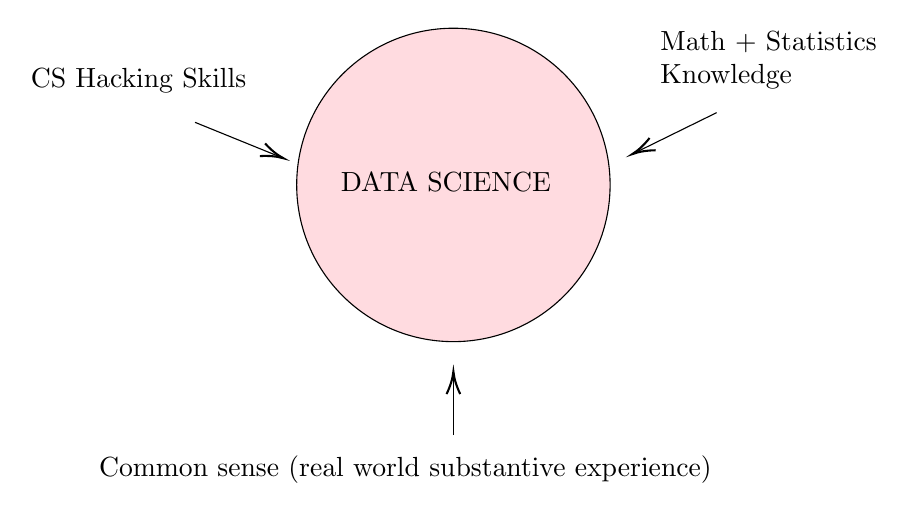
\begin{tikzpicture}[x=0.75pt,y=0.75pt,yscale=-1,xscale=1]
%uncomment if require: \path (0,300); %set diagram left start at 0, and has height of 300

%Shape: Circle [id:dp061140258122834745] 
\draw  [fill={rgb, 255:red, 255; green, 219; blue, 224 }  ,fill opacity=1 ] (254.67,119.5) .. controls (254.67,77.8) and (288.47,44) .. (330.17,44) .. controls (371.86,44) and (405.67,77.8) .. (405.67,119.5) .. controls (405.67,161.2) and (371.86,195) .. (330.17,195) .. controls (288.47,195) and (254.67,161.2) .. (254.67,119.5) -- cycle ;
%Straight Lines [id:da4450208385410075] 
\draw    (205.67,89.33) -- (246.48,105.91) ;
\draw [shift={(248.33,106.67)}, rotate = 202.11] [color={rgb, 255:red, 0; green, 0; blue, 0 }  ][line width=0.75]    (10.93,-3.29) .. controls (6.95,-1.4) and (3.31,-0.3) .. (0,0) .. controls (3.31,0.3) and (6.95,1.4) .. (10.93,3.29)   ;
%Straight Lines [id:da055339322100053545] 
\draw    (457,84.67) -- (418.13,103.78) ;
\draw [shift={(416.33,104.67)}, rotate = 333.81] [color={rgb, 255:red, 0; green, 0; blue, 0 }  ][line width=0.75]    (10.93,-3.29) .. controls (6.95,-1.4) and (3.31,-0.3) .. (0,0) .. controls (3.31,0.3) and (6.95,1.4) .. (10.93,3.29)   ;
%Straight Lines [id:da5012858238681945] 
\draw    (330.17,240) -- (330.17,211.33) ;
\draw [shift={(330.17,209.33)}, rotate = 450] [color={rgb, 255:red, 0; green, 0; blue, 0 }  ][line width=0.75]    (10.93,-3.29) .. controls (6.95,-1.4) and (3.31,-0.3) .. (0,0) .. controls (3.31,0.3) and (6.95,1.4) .. (10.93,3.29)   ;

% Text Node
\draw (274.67,112.5) node [anchor=north west][inner sep=0.75pt]   [align=left] {DATA SCIENCE};
% Text Node
\draw (125.33,62) node [anchor=north west][inner sep=0.75pt]   [align=left] {CS Hacking Skills};
% Text Node
\draw (428.67,44.33) node [anchor=north west][inner sep=0.75pt]   [align=left] {Math + Statistics\\Knowledge};
% Text Node
\draw (158.17,248.67) node [anchor=north west][inner sep=0.75pt]   [align=left] {Common sense (real world substantive experience)};


\end{tikzpicture}

}

\subsection{Topics}

Here are the general topics that this class will cover.

\begin{itemize}
	\item Processing data
	\item Visualizing data
	\item Understanding data
	\item Communicating data
	\item Extracting value from data
\end{itemize}

\subsection{Tools}

Here are some tools commonly employed by data scientists. We'll try to cover how to use most of them here.

\begin{itemize}
	\item Python
	\item Scikit-Learn
	\item Docker
	\item PANDAS
	\item Spark
	\item TensorFlow
\end{itemize}

\subsection{Conda}

Conda is a package and environment manager for python that we can use with the command line.
We can create multiple environments for us and install separate packages in each of them.
This will be highly useful to us, as we sometimes want to consolidate the tools we use into separate environments.

\section{Lecture 2}

\begin{tcolorbox}[title=Definition:,colframe=red!75!black,colback=red!5!white,arc=0pt,fonttitle=\bfseries]
\textbf{Data Collection} $\rightarrow$ The process of measuring and gathering information on targeted variables.
\end{tcolorbox}

\subsection{Literate Programming}

The idea of \textbf{literate programming} is that you have the source code, an explanation of the source code, and the end result of running the code all in one file. Usually, this file is identified as a \textit{notebook}. In other words, the syntax is no different from regular code, you just get a more organized way to show off tables, plots, and other outputs generated from your code.

\subsection{Jupyter Notebook + Alternatives}

Jupyter Notebook is a service that started off as \texttt{iPython}, but it's basically a web-based platform that we use for literate programming. Specifically, it supports Python-based literate programming. Most data scientists prefer it, and it can also apparently leverage big data tools, such as Apache Spark.\newline

It saves files in \texttt{.ipynb} format, which most platforms (i.e. GitHub) have built in viewers for. Options to export in other readable formats are available. Basically, it's just Python with a bunch of bells and whistles on top to make the output of your code look pretty.\newline

\textit{Apache Zeppelin} is an alternative data analysis tool, but we will stick to Jupyter for our purposes. This is because Jupyter seems to be preferred in industry.\newline

\textit{RStudio} is the equivalent, for people who prefer to use the \texttt{R} programming language for data science.\newline

This course will be centered around Jupyter Notebook.

\subsection{List Comprehensions in Python}

To make lists in Python, you can use loops or the \texttt{map()} function, but a \textit{pythonic} way of doing this would be to use a list comprehension. Below is a simple example.\newline

\begin{myproof}
\textbf{Example:} Make a list of all the squares of \texttt{\{0,1,2,3,4,5,6,7,8,9\}}\newline\newline
\textbf{List Comprehension:}\newline
\texttt{squares = [i * i for i in range(10)]}
\end{myproof}

A good way of thinking about this is that it allows you to build sets like a mathematician. This is a common theme in data science, where we can find the intersection between a lot of math stuff and computer science stuff. It's good to know how lists are generated in a mathematical sense in Python for that reason. Here's an example where we translate mathematical notation into a Python list comprehension.\\

\begin{myproof}
\textbf{Example:} Make a list of all odd natural numbers from 0 to 999\\\\
\textbf{Math Notation:}\\ $E =$ \{$x$ | $x$ in $\mathbb{N} \land x$ is odd $\land x<1000$ \}\\\\
\textbf{List Comprehension:}\\
\texttt{E = [x for x in range(1000) if x \% 2 != 0]}
\end{myproof}

\subsection{Using Python3}

We will use Python3. Since I used Python2 during my internship, I'm going to note some big changes to keep track of.\\

\begin{itemize}
	\item Python3 is backwards incompatible. (Don't write in Python2!)
	\item Print has changed from a command to a function, so make sure to use proper function notation when invoking it.
	\item Division has changed. \texttt{1/2} no longer equals 0. \texttt{1/2 == 0.5} and floored division is now taken care of this way: \texttt{1//2 == 0}
\end{itemize}

\subsection{Python vs. R for Data Scientists}

Some arguments for both sides in terms of what to use.

\begin{itemize}
	\item Python is a 'full' programming langauge. Also, if you've got prior experience with Python paradigms or just programming in general, that's a big plus in terms of learning curve.
	\item R has more mature 'pure statistics' libraries, but Python is apparently catching up.
	\item In terms of \textbf{processing speed}, R is certainly faster. It was designed and optimized for statistics processing.
	\item Python is preferable for machine learning operations, which is pretty big right now.
\end{itemize}

My personal choice will be to use Python as much as I can when I'm studying this course. Since it's more prominent in the tech industry, I should be using it more anyway.

\subsection{The Classic Statistical View of Data}

There are \textbf{four} main types of data: Nominal, Ordinal, Interval, and Ratio data. They can each be classified under two main subgroups, Categorical and Numerical data. Here's a visualization.\\

{
\centering



\tikzset{every picture/.style={line width=0.75pt}} %set default line width to 0.75pt        

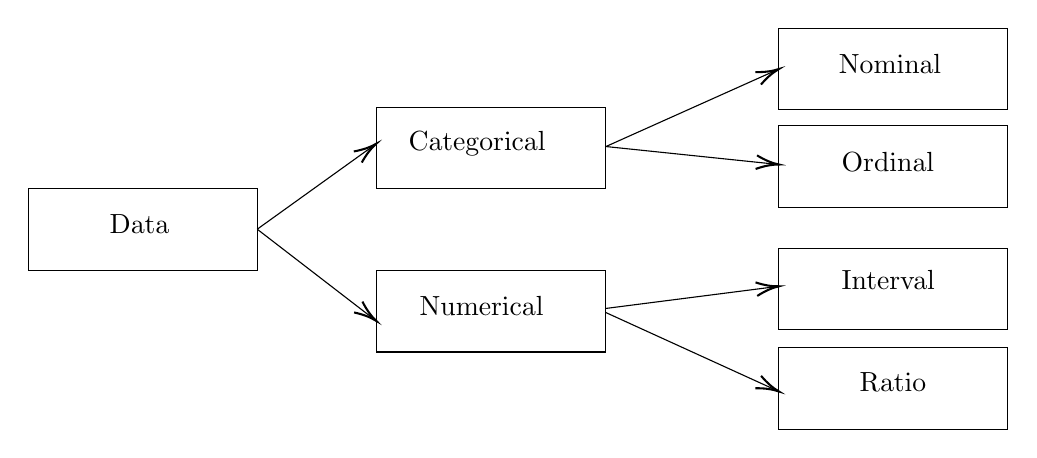
\begin{tikzpicture}[x=0.75pt,y=0.75pt,yscale=-1,xscale=1]
%uncomment if require: \path (0,300); %set diagram left start at 0, and has height of 300

%Shape: Rectangle [id:dp8149613399348021] 
\draw   (72,131) -- (182.33,131) -- (182.33,170.33) -- (72,170.33) -- cycle ;
%Shape: Rectangle [id:dp680618887900226] 
\draw   (239.67,91.67) -- (350,91.67) -- (350,131) -- (239.67,131) -- cycle ;
%Shape: Rectangle [id:dp777477779359951] 
\draw   (239.67,170.33) -- (350,170.33) -- (350,209.67) -- (239.67,209.67) -- cycle ;
%Shape: Rectangle [id:dp9580214955547155] 
\draw   (433.67,53.67) -- (544,53.67) -- (544,93) -- (433.67,93) -- cycle ;
%Shape: Rectangle [id:dp19525566557447283] 
\draw   (433.67,100.5) -- (544,100.5) -- (544,139.83) -- (433.67,139.83) -- cycle ;
%Shape: Rectangle [id:dp18958725273981114] 
\draw   (433.67,159.67) -- (544,159.67) -- (544,199) -- (433.67,199) -- cycle ;
%Shape: Rectangle [id:dp27616820331988945] 
\draw   (433.67,207.67) -- (544,207.67) -- (544,247) -- (433.67,247) -- cycle ;
%Straight Lines [id:da07504069427898741] 
\draw    (182.33,150.5) -- (238.04,110.5) ;
\draw [shift={(239.67,109.33)}, rotate = 504.32] [color={rgb, 255:red, 0; green, 0; blue, 0 }  ][line width=0.75]    (10.93,-3.29) .. controls (6.95,-1.4) and (3.31,-0.3) .. (0,0) .. controls (3.31,0.3) and (6.95,1.4) .. (10.93,3.29)   ;
%Straight Lines [id:da18494381831895634] 
\draw    (182.33,150.5) -- (238.08,193.45) ;
\draw [shift={(239.67,194.67)}, rotate = 217.61] [color={rgb, 255:red, 0; green, 0; blue, 0 }  ][line width=0.75]    (10.93,-3.29) .. controls (6.95,-1.4) and (3.31,-0.3) .. (0,0) .. controls (3.31,0.3) and (6.95,1.4) .. (10.93,3.29)   ;
%Straight Lines [id:da49166239871511697] 
\draw    (350.33,110.67) -- (431.84,74.15) ;
\draw [shift={(433.67,73.33)}, rotate = 515.87] [color={rgb, 255:red, 0; green, 0; blue, 0 }  ][line width=0.75]    (10.93,-3.29) .. controls (6.95,-1.4) and (3.31,-0.3) .. (0,0) .. controls (3.31,0.3) and (6.95,1.4) .. (10.93,3.29)   ;
%Straight Lines [id:da6935259459415319] 
\draw    (350.33,110.67) -- (431.68,119.13) ;
\draw [shift={(433.67,119.33)}, rotate = 185.94] [color={rgb, 255:red, 0; green, 0; blue, 0 }  ][line width=0.75]    (10.93,-3.29) .. controls (6.95,-1.4) and (3.31,-0.3) .. (0,0) .. controls (3.31,0.3) and (6.95,1.4) .. (10.93,3.29)   ;
%Straight Lines [id:da6050313931467277] 
\draw    (350.33,190.67) -- (431.85,227.84) ;
\draw [shift={(433.67,228.67)}, rotate = 204.51] [color={rgb, 255:red, 0; green, 0; blue, 0 }  ][line width=0.75]    (10.93,-3.29) .. controls (6.95,-1.4) and (3.31,-0.3) .. (0,0) .. controls (3.31,0.3) and (6.95,1.4) .. (10.93,3.29)   ;
%Straight Lines [id:da8985137963347964] 
\draw    (350.33,188.67) -- (431.68,178.25) ;
\draw [shift={(433.67,178)}, rotate = 532.71] [color={rgb, 255:red, 0; green, 0; blue, 0 }  ][line width=0.75]    (10.93,-3.29) .. controls (6.95,-1.4) and (3.31,-0.3) .. (0,0) .. controls (3.31,0.3) and (6.95,1.4) .. (10.93,3.29)   ;

% Text Node
\draw (110,142.17) node [anchor=north west][inner sep=0.75pt]   [align=left] {Data};
% Text Node
\draw (254,102) node [anchor=north west][inner sep=0.75pt]   [align=left] {Categorical};
% Text Node
\draw (259.33,181.33) node [anchor=north west][inner sep=0.75pt]   [align=left] {Numerical};
% Text Node
\draw (461.33,65) node [anchor=north west][inner sep=0.75pt]   [align=left] {Nominal};
% Text Node
\draw (462.67,112) node [anchor=north west][inner sep=0.75pt]   [align=left] {Ordinal};
% Text Node
\draw (462.67,168.83) node [anchor=north west][inner sep=0.75pt]   [align=left] {Interval};
% Text Node
\draw (471.33,218.33) node [anchor=north west][inner sep=0.75pt]   [align=left] {Ratio};


\end{tikzpicture} \\
}

\subsubsection{Nominal Data}

A type of categorical data, nominal data value have names and describe the state of things. For example, your marriage status is nominal data because you can either be \textit{single}, \textit{married}, or \textit{separated}. Another example is the type of drink you're going to have. Will it be \textit{Milk}, \textit{Beer}, or \textit{Juice}?\\

The key here is that there can be no quantitative values assigned to each of these categories, as that would allow us to do math with them and would defeat the purpose of these labels. These values \textbf{cannot be easily compared}, so they have no material value. \textit{E.g. being single is not quantitatively better than being married (objectively), and vice versa}.\\

\begin{myproof}
\textbf{Example:} What is your marital status?
\begin{itemize}
	\item Married
	\item Divorced (separated)
	\item Single
\end{itemize}
\end{myproof}

\subsubsection{Ordinal Data}

Ordinal data represents values that have names that describe the state of things, but in this case, there \textbf{is} an ordering of those values. This is what sets it apart from nominal data. \\ 
\begin{myproof}
\textbf{Example:} What did you think of the movie?
\begin{itemize}
	\item Strongly liked
	\item Liked
	\item Indifferent
	\item Disliked
	\item Strongly Disliked
\end{itemize}
\end{myproof}

Given how subjective some of these things can be, the distinction between nominal and ordinal can be \textbf{blurry} at times. For example, going back to our nominal example, some people may think that being single is quantitatively better than being married.

\subsubsection{Interval and Ratio Data}

Interval and Ratio data are pretty similar, and both can be used to measure things that can be represented by either integers or real numbers. \\

\textbf{Interval} data scales with fixed but arbitrary values. That might sound silly, but a good example is \textbf{dates}. Below is an example of two data comparisons of interval data that seem arbitrary, but indeed hold integer value.\\

\begin{myproof}
\textbf{Example:} The following two operations are equal. \\\\
\texttt{10/1/2019 - 9/1/2019} \\
\texttt{10/1/2018 - 9/1/2018}
\end{myproof}

The measures don't look like integer values at first, but we can quantify them by marking them with days.\\

Here's what sets \textbf{Interval} data apart, however. You have \textbf{no method} of computing ratios or scales with it. For example, never mind that you can try computing \texttt{(9/1/2019 $\times$ 8/25/2015)}, the unit of the answer would be totally useless to us, and neither would the actual number, even if you went ahead with the operation.\\

\textbf{Ratio} data is, in essence, the same as interval data in that it is numerical, but the scale itself \textbf{has a true zero}. While dates don't necessarily have a true zero, we can say that money counts as ratio data. For example, having zero money means that you're at the absolute zero of that scale, whereas the absolute zero for dates is disputable. Are we saying we're starting at O A.D.? The Big Bang? Even earlier?\\

Differentiating between the two is usually a case-by-case basis thing, which is what I'm thinking is the best way to handle any conflicts I end up running into between ratio and interval data.\\

\begin{myproof}
\textbf{Example:} Interval data \\\\
Temperature on the scale of Celsius or Fahrenheit is interval-type data because $0\degree$ is set to an arbitrarily fixed point. Also, we can't scale it properly- $30\degree F$ isn't twice as hot as $15\degree F$.\\\\
\textbf{Example:} Ratio data \\\\
Temperature on the Kelvin scale is ratio data. $0K$ is set at legitimate absolute zero, and $50K$ is truly twice as cold as $100K$.
\end{myproof}

\subsection{Data Science at a Glance}

Data science is basically manipulating and computing using data. As such, we need to shift our thinking from writing \textbf{imperative} code to manipulate \textbf{data structures} to creating \textbf{sequences and pipelines} to conduct operations on \textbf{data}. That stuff is covered more in 420 and 424, for reference.\newline

More often than not, we have to take the data that we've found and make it easily understandable for humans. This is called Data Representation.\newline

\begin{tcolorbox}[title=Definition:,colframe=red!75!black,colback=red!5!white,arc=0pt,fonttitle=\bfseries]
\textbf{Data Representation} $\rightarrow$ The natural way to think about data, in a human way.
\end{tcolorbox}

Here are some ways that we think about data in this class:\newline

\begin{itemize}
	\item \textbf{One Dimensional Arrays} $\rightarrow$ E.g. \texttt{<'red', 'blue', 'green'>} or \texttt{<0,3,4>}. We can use functions like map, fold and filter to manipulate these.
	\item \textbf{N-Dimensional Arrays} $\rightarrow$ Also known as \textbf{tensors}.
	\begin{itemize}
		\item For example, a Tensor of dimensions \texttt{[6,4]} is just a $6\times 4$ matrix.
		\item Similarly, a Tensor of dimensions \texttt{[4,4,2]} is a 3D array.
		\item Here, we can start to make use of \textbf{Linear Algebra} for further data manipulation. Some example operations that we can use to mess with tensors:
		\begin{itemize}
			\item Matrix/Tensor Multiplications
			\item Transpose
			\item Vector Multiplication
			\item Matrix Factorization (we will explore this later)
		\end{itemize}
	\end{itemize}
	\item \textbf{Sets} of objects, or \textbf{Key/Value Pairs}
	\item \textbf{Tables/Relations} $\rightarrow$ This goes into relational databases, which is the basis of \texttt{SQL}. We'll go into this later.
	\item \textbf{Hierarchies/Trees/Graphs} $\rightarrow$ This sort of spills over into data structures, but they've got some additional nuances included with them.
	\begin{itemize}
		\item They tend to make use of 'path' queries
		\item Graph and Tree Algorithms will be useful here, efficiency is key
		\item Example: networks are represented this way, we'll cover that later in this class
	\end{itemize}
\end{itemize}

\section{Lecture 3}

\subsection{Acquiring Data}

Here are some examples of how we can grab data from places. Pretty obvious, common sense stuff. We're going to explore all of these as we move forward.

\begin{itemize}
	\item Direct download from online or loading it from local storage
	\item Generate the data locally via a simulation or equivalent program
	\item Query data from a database 
	\item Query data from an API
	\item Scrape data from a website
\end{itemize}

When you pull from APIs, you're going to want to be using HTTP Requests.

\subsection{RESTful APIs}

This stands for REpresentational State Transfer APIs, and it's basically a standard that enforces that APIs do a few things. It says that they should support these basic operations:

\begin{itemize}
	\item \texttt{GET} $\rightarrow$ Query a data entry
	\item \texttt{POST} $\rightarrow$ Create a new data entry
	\item \texttt{PUT} $\rightarrow$ Update an existing data entry
	\item \texttt{DELETE} $\rightarrow$ Delete an existing data entry
\end{itemize}

RESTful APIs are also supposed to be stateless. That is, with every API request, you send a token of who you are, and you get a current capture of the data at that time/edit the data.\newline

A good example of a REST API is Github, where you can use REST API calls on your repositories.\newline

There are other guiding principles and miscellaneous guidelines for RESTful APIs, which can all be found at \texttt{https:/restfulapi.net}\newline

\begin{tcolorbox}[title=Aside: GRAPHQL,colframe=black,colback=white,arc=0pt,fonttitle=\bfseries]
\textbf{GraphQL} $\rightarrow$ REST has been adopted by many developers and is widely regarded as the traditional way to send data over HTTP. GraphQL, on the other hand, is a revolutionary new player that's presented as a way to \textit{replace} legacy REST APIs \textit{(back4apps)}
\end{tcolorbox}

\subsection{Oauth}

If you want to grant an app access to your identity without actually giving it your username and password, is there a way to do that? The answer is \textbf{yes}, because this is a common software engineering problem.\newline

\textbf{OAuth} is the standard for \textit{access delegation} used for internet users to grant websites access to their information on other sites. A pretty good example of this is Google's sign in page on other websites. How do you think other websites conduct sign in without knowing your password for your Google account?

\subsection{GET Requests}

Assume we used Python's \texttt{requests} module to query a server with a \texttt{GET} request.\newline

First, we'd get either a \texttt{CSV}, \texttt{JSON}, or \texttt{HTML/XML/XHTML} file back, in response. This is the data that we have to sift through. \textit{Note:} You might also get a domain-specific file, like an \textbf{rvt} file. You're always welcome to make your own filetype for storing data, but make sure it's actually documented somewhere.\newline

\begin{tcolorbox}[title=Aside: Parsing CSVs and JSON,colframe=black,colback=white,arc=0pt,fonttitle=\bfseries]
Never write your own \texttt{CSV} or \texttt{JSON} parsers. This is another example of reinventing the wheel. We'll use Python Libraries to do this more easily. \textit{E.g. PANDAS}
\end{tcolorbox}

\subsection{More on Data Storage Formats}

\begin{tcolorbox}[title=Definition:,colframe=red!75!black,colback=red!5!white,arc=0pt,fonttitle=\bfseries]
\textbf{Serialization} $\rightarrow$ The process of converting objects into strings.\newline
\textbf{Deserialization} $\rightarrow$ The process of converting strings back into objects.
\end{tcolorbox}

\textbf{\texttt{JSON}} is a pretty common format for serializing objects. Plus, serializing objects makes it easier for humans to read and perform sanity-checks on. In Python, \texttt{JSON} is built with Strings, Lists, Dictionaries, and sometimes mixes of a few of those together.\newline

\begin{tcolorbox}[title=Definition:,colframe=red!75!black,colback=red!5!white,arc=0pt,fonttitle=\bfseries]
\textbf{Document Object Model} $\rightarrow$ A tree-based data storage method. For example, HTML is structured this way.
\end{tcolorbox}

\subsubsection{SAX}

SAX is a lightweight way to process XML. It generates a stream of events as it parses an XML file. IT helps us pay attention to individual parts of an XML file without having to process through the rest of it.

\subsection{Parsing HTML}

Parsing HTML is the hardest to do in this case, as I've seen many times before in hackathon projects. Although HTML's specifications are pure, the real world examples of it are pretty nightmarish, thanks to how it interacts with JavaScript and loads dynamic content. All in all, it's fairly unreliable in terms of parsing it manually.\newline

In this case, we're best off using the Python library \texttt{BeautifulSoup}. We can also make use of Python's Regex, which is similar enough to Ruby regex that we worked with in 330. A website like Rubular-\texttt{https://pythex.org} will be useful in this case.\newline

By combining \texttt{BeautifulSoup}, Regular expressions, and \texttt{GET} requests, we can make the process fairly streamlined. This is usually what we'll be using to scrape websites. In order to scrape more dynamic websites, we'd probably have to make use of Selenium. Check my 320 folder to find an example of a simple webscraper with \texttt{BeautifulSoup}.

\section{Lecture 4}

\textbf{Overview:} \textbf{Numpy, PANDAS, Relational Databases, Apache Spark}\newline

\subsection{Available Technologies}

Python has a bunch of 3rd party packages for scientific and numerical computation. Some examples are..

\begin{itemize}
	\item \textbf{\texttt{Numpy} and \texttt{Scipy}} $\rightarrow$ Numerical and scientific function libraries.
	\item \textbf{\texttt{NUMBA}} $\rightarrow$ A Python compiler supporting 'Just in Time' compilation. That is, it supports compilation of code while code is running.
	\item \textbf{\texttt{ALGLIB}} $\rightarrow$ A cross-platform numerical analysis library
	\item \textbf{\texttt{PANDAS}} $\rightarrow$ An extensive data analysis tool with some neat built-in data structures
	\item \textbf{\texttt{PyGSL}} $\rightarrow$ GNU Scientific Library in Python
	\item \textbf{Scientific Python} $\rightarrow$ A collection of scientific computing modules for Python
\end{itemize}

These are a bunch of examples of what's available to developers right now, but we won't focus on all of it. Particular emphasis will be placed on \texttt{Numpy} and \texttt{PANDAS}.

\subsection{NumPy Stack}

The \textbf{NumPy} stack is the most commonly used out of all of these packages. It includes the following:

\begin{itemize}
	\item \texttt{Numpy} - Works sort of like MatLab, just lets us handle a lot of number manipulation and mathematical operations
	\item \texttt{Matplotlib} - This is a plotting and graphing library
	\item \texttt{PANDAS} - This gives us a bunch of data structures and data analysis tools to play with/keep track of our data. (Usually, you'll want to import your data into a \texttt{PANDAS} \texttt{dataframe} or something.)
	\item \texttt{SciPy}
	\item \texttt{SymPy}
	\item \texttt{Jupyter} - This will be our medium for \textbf{literate programming}.
\end{itemize}

To see more about this stuff, search Google for the \textbf{NumPy Stack} and you'll find everything you need.

\subsubsection{Misc About NumPy}

Here are a few more notable things about \texttt{Numpy}:

\begin{itemize}
	\item It contains the \textbf{n-dimensional array} object
	\item It contains 'sophisticated' functions that we can use
	\item It provides us with excellent tools to integrate \texttt{C++}, \texttt{C}, and even \texttt{FORTRAN}
	\item It has math capabilities that are highly useful to us (e.g. Linear Algebra, Fourier Transform, etc)
	\item \texttt{Numpy} also comes with a bunch of new DataTypes for us to use.
\end{itemize}

\begin{tcolorbox}[title=Aside: Numpy Arrays,colframe=black,colback=white,arc=0pt,fonttitle=\bfseries]
Arrays in \texttt{Numpy} are different from regular lists in Python, so make sure your syntax is correct and you know the difference when you decide to use either one in practice.
\end{tcolorbox}

\subsubsection{Linear Algebra with NumPy}

One of \texttt{NumPy}'s most common uses lies within its \textbf{Linear Algebra} module. It allows us to do regular LA stuff, like \texttt{.transpose()} and \texttt{.inverse()} to matrices stored as n-dim arrays. Here's an example.

{\centering
\begin{lstlisting}[language=python]
# Note: remember, we have to use NumPy's n-dimensional array object here

array([[1.0, 2.0],
       [3.0, 4.0]]).transpose()
\end{lstlisting}
}

\subsubsection{SciPy}

\textbf{\texttt{SciPy}} includes various tools and functions for solving common problems in \textbf{scientific computing}.\\

We won't use it much for now, but it's supposed to be good to know. Often you'll be able to find higher-level \texttt{Scipy} functions that will work around the need to call lower-level \texttt{Scipy} functions. It's got a lot of functionality built in, so make sure not to overlook it.

\subsection{The Idea of Reproducibility}

Starting from the same dataset, can we reproduce your analysis and get the same results? \textbf{This is the goal that we're trying to fulfill with our analysis}- we want our stuff to be reproducible! (Otherwise, what exactly does it even mean?)

\subsection{Best Practices}

Honestly, most of this stuff should be common sense.

\begin{itemize}
	\item Use version control to keep track of code. (e.g. \texttt{git})
	\item Use unit testing. (e.g. \texttt{unittest} module in python)
	\item Use libraries when you can. (don't reinvent the wheel!)
\end{itemize}

\subsection{The Idea of Open Data}

Some data should be widely available for everyone to use as they want, without restrictions from copyright, etc.\\

This is probably where all of our free data comes from, so this idea is super helpful to us as data scientists.

\subsection{General Process}

Here's the general process for data science- just so we have an idea of what's going on.\\



\tikzset{every picture/.style={line width=0.75pt}} %set default line width to 0.75pt        

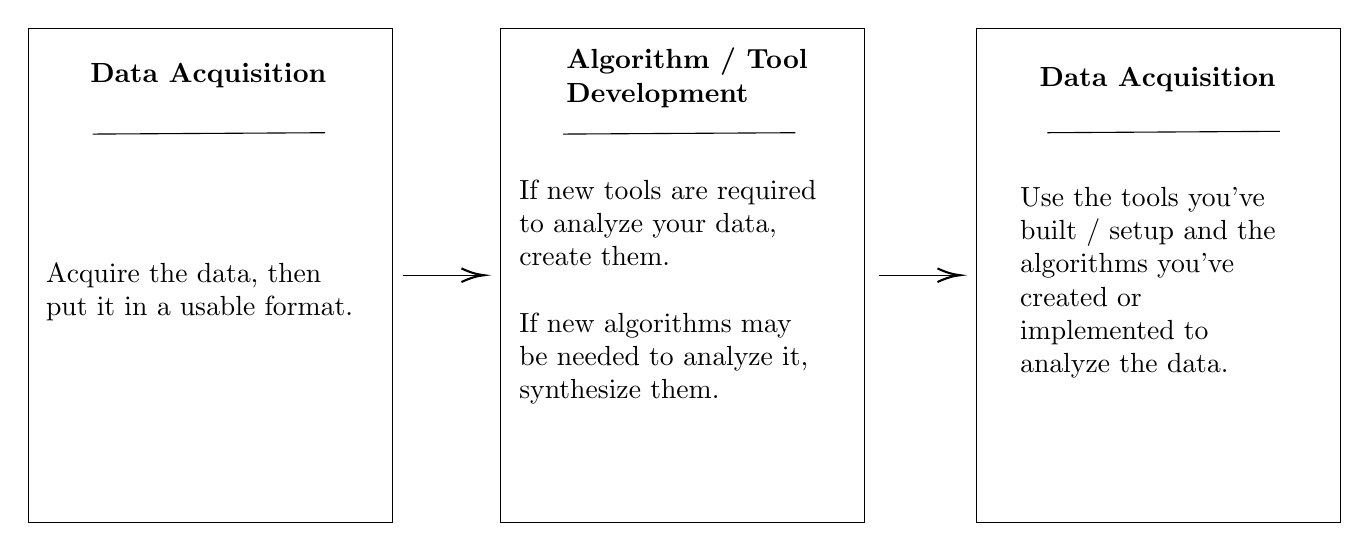
\begin{tikzpicture}[x=0.75pt,y=0.75pt,yscale=-1,xscale=1]
%uncomment if require: \path (0,300); %set diagram left start at 0, and has height of 300

%Shape: Rectangle [id:dp9523245055647409] 
\draw   (34.67,19.33) -- (210.33,19.33) -- (210.33,257.33) -- (34.67,257.33) -- cycle ;
%Shape: Rectangle [id:dp26296611780141976] 
\draw   (262,19.33) -- (437.67,19.33) -- (437.67,257.33) -- (262,257.33) -- cycle ;
%Shape: Rectangle [id:dp4749898829673477] 
\draw   (491.33,19.33) -- (667,19.33) -- (667,257.33) -- (491.33,257.33) -- cycle ;
%Straight Lines [id:da3772898435405757] 
\draw    (65.67,70.33) -- (177.67,69.67) ;
%Straight Lines [id:da47086799536926727] 
\draw    (292.33,70.33) -- (404.33,69.67) ;
%Straight Lines [id:da16258158592667293] 
\draw    (525.67,69.67) -- (637.67,69) ;
%Straight Lines [id:da8259565971285442] 
\draw    (215,138.33) -- (252.33,138.33) ;
\draw [shift={(254.33,138.33)}, rotate = 180] [color={rgb, 255:red, 0; green, 0; blue, 0 }  ][line width=0.75]    (10.93,-3.29) .. controls (6.95,-1.4) and (3.31,-0.3) .. (0,0) .. controls (3.31,0.3) and (6.95,1.4) .. (10.93,3.29)   ;
%Straight Lines [id:da6335608206253658] 
\draw    (444.33,138.33) -- (481.67,138.33) ;
\draw [shift={(483.67,138.33)}, rotate = 180] [color={rgb, 255:red, 0; green, 0; blue, 0 }  ][line width=0.75]    (10.93,-3.29) .. controls (6.95,-1.4) and (3.31,-0.3) .. (0,0) .. controls (3.31,0.3) and (6.95,1.4) .. (10.93,3.29)   ;

% Text Node
\draw (63.33,35) node [anchor=north west][inner sep=0.75pt]   [align=left] {\textbf{Data Acquisition}};
% Text Node
\draw (292.67,27.67) node [anchor=north west][inner sep=0.75pt]   [align=left] {\textbf{Algorithm / Tool}\\\textbf{Development}};
% Text Node
\draw (520.67,37) node [anchor=north west][inner sep=0.75pt]   [align=left] {\textbf{Data Acquisition}};
% Text Node
\draw (42,131.33) node [anchor=north west][inner sep=0.75pt]   [align=left] {Acquire the data, then\\put it in a usable format.};
% Text Node
\draw (270,91.33) node [anchor=north west][inner sep=0.75pt]   [align=left] {If new tools are required\\to analyze your data,\\create them.\\\\If new algorithms may\\be needed to analyze it,\\synthesize them.};
% Text Node
\draw (511.33,94.67) node [anchor=north west][inner sep=0.75pt]   [align=left] {Use the tools you've\\built / setup and the \\algorithms you've \\created or \\implemented to \\analyze the data.};


\end{tikzpicture}

\hfill \break After we do that, we still technically have some programming left. In this new era of literate programming, there's one more step of processing we have to do with our results in order to make them publicly presentable and meaningful.\\



\tikzset{every picture/.style={line width=0.75pt}} %set default line width to 0.75pt        

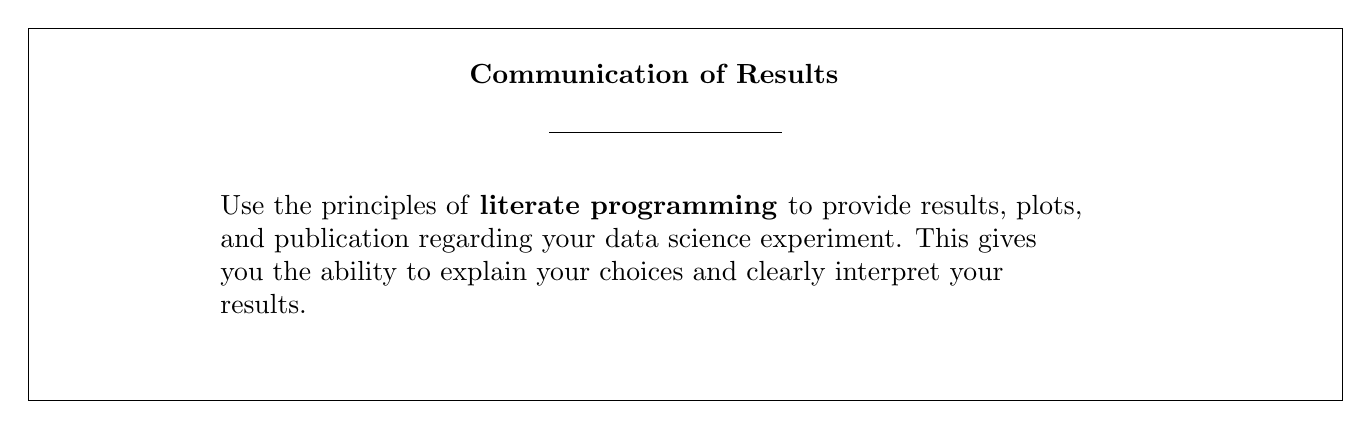
\begin{tikzpicture}[x=0.75pt,y=0.75pt,yscale=-1,xscale=1]
%uncomment if require: \path (0,300); %set diagram left start at 0, and has height of 300

%Shape: Rectangle [id:dp9523245055647409] 
\draw   (34.67,19.33) -- (667.67,19.33) -- (667.67,198.67) -- (34.67,198.67) -- cycle ;
%Straight Lines [id:da3772898435405757] 
\draw    (285.67,69.67) -- (397.67,69.67) ;

% Text Node
\draw (246,35.67) node [anchor=north west][inner sep=0.75pt]   [align=left] {\textbf{Communication of Results}};
% Text Node
\draw (126,98.33) node [anchor=north west][inner sep=0.75pt]   [align=left] {Use the principles of \textbf{literate programming }to provide results, plots,\\and publication regarding your data science experiment. This gives\\you the ability to explain your choices and clearly interpret your\\results.};


\end{tikzpicture}


\hfill \break It's emphasized a lot here to think like an \textbf{algorithm developer}, as you're going to need efficiency in the data analysis that you perform. However, you also need to think like an experiment-conducting \textbf{data scientist}. We don't usually get enough training as the latter, so hopefully this course should be an introduction to that sort of stuff.

\subsection{Project Organization}

Make sure to organize your project in folders appropriately. Specifically, even if you have a lot of components, group with with a focus on experimental procedure.\\

You should certainly be isolating things like \textbf{data}, \textbf{tools}, and \textbf{experiments} into their own folders. Data could include your raw input data, along with data that you've done some processing on. Tools could include Python environment you're using, and experiments could include the meat of what your data science work will be- pipeline scripts, results, figures, plots, analysis scripts, etc.

\subsection{A Little on Bias, Ethics, Responsibility}

\begin{tcolorbox}[title=Aside: Fairness Through Blindness,colframe=black,colback=white,arc=0pt,fonttitle=\bfseries]
The concept of not letting an algorithm look at protected attributes in order to keep it from forming potentially harmful biases.
\end{tcolorbox}

\hfill \break A great example of fairness through blindness could be software that determines the outcome for a loan application. We want the results to be \textbf{independent} of an applicant's race, but they can be \textbf{dependent} on non-protected attributes, such as credit history and income.\\

\begin{tcolorbox}[title=Aside: FATML,colframe=black,colback=white,arc=0pt,fonttitle=\bfseries]
\textbf{FATML} stands for Fairness, Accountability, and Transparency in Machine Learning.
\end{tcolorbox}

\hfill \break Overall, here are some guiding principles for data ethics:

\begin{itemize}
	\item Start with clear user need, with a focus on public benefit. (Can't go wrong with this!)
	\item Use data and tools that emphasize \textbf{minimum} intrusion/invasion of privacy. (Sometimes, we have no choice but to handle sensitive data)
	\item Create robust data science models that minimize bias and focus on objective accuracy.
	\item Be alert to public perceptions.
	\item Be open and accountable for your actions.
	\item Security is key- especially if working with sensitive data.
\end{itemize}

\section{Lecture 5 \& 6}

\textbf{Big ideas: Pandas + Relational Databases}

\begin{itemize}
	\item Tables (Specifically, the abstraction + operations)
	\item \texttt{PANDAS}
	\item The idea of 'tidy' data
	\item \texttt{SQL}
\end{itemize}

\subsection{Tables}

Here's the idea- we can abstract data into our own little data structures just like computer scientists do, and a lot of the time, in data science, tables are the optimal way to do that. (This is why software like PANDAS and Numpy have excellent support for these structures.)\\

{
\centering



\tikzset{every picture/.style={line width=0.75pt}} %set default line width to 0.75pt        

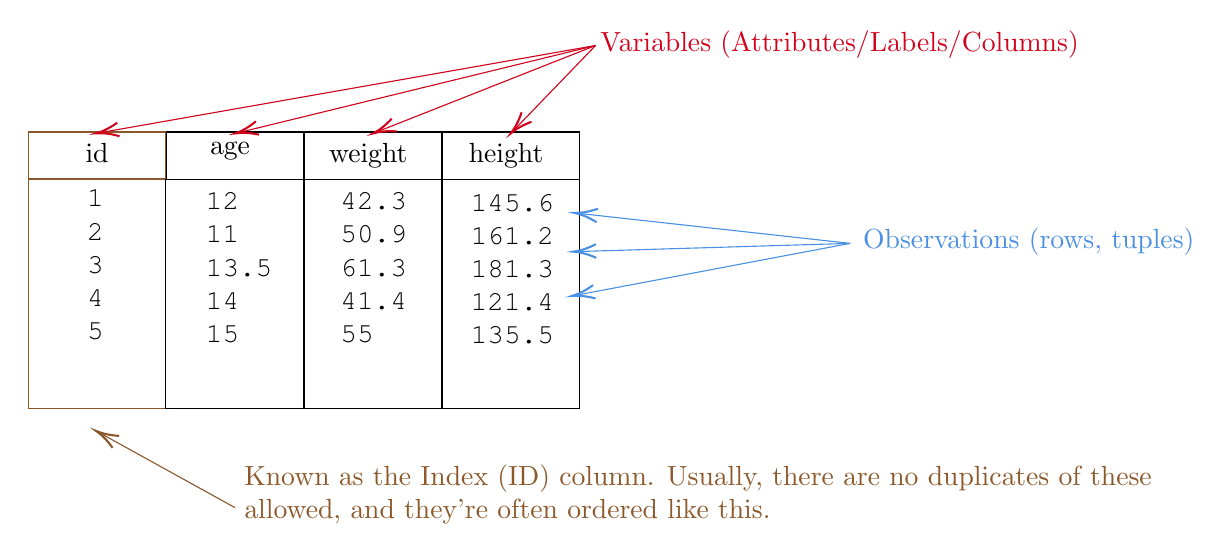
\begin{tikzpicture}[x=0.75pt,y=0.75pt,yscale=-1,xscale=1]
%uncomment if require: \path (0,300); %set diagram left start at 0, and has height of 300

%Shape: Rectangle [id:dp5949882099932227] 
\draw  [color={rgb, 255:red, 139; green, 87; blue, 42 }  ,draw opacity=1 ] (52.33,67.67) -- (118.67,67.67) -- (118.67,90.67) -- (52.33,90.67) -- cycle ;
%Shape: Rectangle [id:dp5180660849056042] 
\draw   (119,67.67) -- (185.33,67.67) -- (185.33,90.67) -- (119,90.67) -- cycle ;
%Shape: Rectangle [id:dp928756418037382] 
\draw   (185,67.67) -- (251.33,67.67) -- (251.33,90.67) -- (185,90.67) -- cycle ;
%Shape: Rectangle [id:dp982011584275448] 
\draw   (251.67,67.67) -- (318,67.67) -- (318,90.67) -- (251.67,90.67) -- cycle ;
%Shape: Rectangle [id:dp4812611593055496] 
\draw  [color={rgb, 255:red, 139; green, 87; blue, 42 }  ,draw opacity=1 ] (52.33,90.33) -- (118.67,90.33) -- (118.67,200.67) -- (52.33,200.67) -- cycle ;
%Shape: Rectangle [id:dp14867838676065692] 
\draw   (118.67,90.67) -- (185,90.67) -- (185,200.67) -- (118.67,200.67) -- cycle ;
%Shape: Rectangle [id:dp7944164207923816] 
\draw   (185.33,90.67) -- (251.67,90.67) -- (251.67,200.67) -- (185.33,200.67) -- cycle ;
%Shape: Rectangle [id:dp6914540924812163] 
\draw   (251.67,90.67) -- (318,90.67) -- (318,200.67) -- (251.67,200.67) -- cycle ;
%Straight Lines [id:da8659955223770235] 
\draw [color={rgb, 255:red, 208; green, 2; blue, 27 }  ,draw opacity=1 ]   (325.67,26) -- (86.97,67.99) ;
\draw [shift={(85,68.33)}, rotate = 350.02] [color={rgb, 255:red, 208; green, 2; blue, 27 }  ,draw opacity=1 ][line width=0.75]    (10.93,-3.29) .. controls (6.95,-1.4) and (3.31,-0.3) .. (0,0) .. controls (3.31,0.3) and (6.95,1.4) .. (10.93,3.29)   ;
%Straight Lines [id:da7649126412714919] 
\draw [color={rgb, 255:red, 208; green, 2; blue, 27 }  ,draw opacity=1 ]   (325.67,26) -- (154.11,67.86) ;
\draw [shift={(152.17,68.33)}, rotate = 346.28999999999996] [color={rgb, 255:red, 208; green, 2; blue, 27 }  ,draw opacity=1 ][line width=0.75]    (10.93,-3.29) .. controls (6.95,-1.4) and (3.31,-0.3) .. (0,0) .. controls (3.31,0.3) and (6.95,1.4) .. (10.93,3.29)   ;
%Straight Lines [id:da04591151144441219] 
\draw [color={rgb, 255:red, 208; green, 2; blue, 27 }  ,draw opacity=1 ]   (325.67,26) -- (220.36,67.6) ;
\draw [shift={(218.5,68.33)}, rotate = 338.44] [color={rgb, 255:red, 208; green, 2; blue, 27 }  ,draw opacity=1 ][line width=0.75]    (10.93,-3.29) .. controls (6.95,-1.4) and (3.31,-0.3) .. (0,0) .. controls (3.31,0.3) and (6.95,1.4) .. (10.93,3.29)   ;
%Straight Lines [id:da1253621546988095] 
\draw [color={rgb, 255:red, 208; green, 2; blue, 27 }  ,draw opacity=1 ]   (325.67,26) -- (286.22,66.89) ;
\draw [shift={(284.83,68.33)}, rotate = 313.97] [color={rgb, 255:red, 208; green, 2; blue, 27 }  ,draw opacity=1 ][line width=0.75]    (10.93,-3.29) .. controls (6.95,-1.4) and (3.31,-0.3) .. (0,0) .. controls (3.31,0.3) and (6.95,1.4) .. (10.93,3.29)   ;
%Straight Lines [id:da7853774637498458] 
\draw [color={rgb, 255:red, 74; green, 144; blue, 226 }  ,draw opacity=1 ]   (448.33,121.33) -- (317.65,106.89) ;
\draw [shift={(315.67,106.67)}, rotate = 366.31] [color={rgb, 255:red, 74; green, 144; blue, 226 }  ,draw opacity=1 ][line width=0.75]    (10.93,-3.29) .. controls (6.95,-1.4) and (3.31,-0.3) .. (0,0) .. controls (3.31,0.3) and (6.95,1.4) .. (10.93,3.29)   ;
%Straight Lines [id:da2813931715021274] 
\draw [color={rgb, 255:red, 74; green, 144; blue, 226 }  ,draw opacity=1 ]   (448.33,121.33) -- (317,125.27) ;
\draw [shift={(315,125.33)}, rotate = 358.28] [color={rgb, 255:red, 74; green, 144; blue, 226 }  ,draw opacity=1 ][line width=0.75]    (10.93,-3.29) .. controls (6.95,-1.4) and (3.31,-0.3) .. (0,0) .. controls (3.31,0.3) and (6.95,1.4) .. (10.93,3.29)   ;
%Straight Lines [id:da28293623689911906] 
\draw [color={rgb, 255:red, 74; green, 144; blue, 226 }  ,draw opacity=1 ]   (448.33,121.33) -- (316.3,146.3) ;
\draw [shift={(314.33,146.67)}, rotate = 349.28999999999996] [color={rgb, 255:red, 74; green, 144; blue, 226 }  ,draw opacity=1 ][line width=0.75]    (10.93,-3.29) .. controls (6.95,-1.4) and (3.31,-0.3) .. (0,0) .. controls (3.31,0.3) and (6.95,1.4) .. (10.93,3.29)   ;
%Straight Lines [id:da8467882522352468] 
\draw [color={rgb, 255:red, 139; green, 87; blue, 42 }  ,draw opacity=1 ]   (152,248.67) -- (86.75,212.63) ;
\draw [shift={(85,211.67)}, rotate = 388.90999999999997] [color={rgb, 255:red, 139; green, 87; blue, 42 }  ,draw opacity=1 ][line width=0.75]    (10.93,-3.29) .. controls (6.95,-1.4) and (3.31,-0.3) .. (0,0) .. controls (3.31,0.3) and (6.95,1.4) .. (10.93,3.29)   ;

% Text Node
\draw (78.67,71.67) node [anchor=north west][inner sep=0.75pt]   [align=left] {id};
% Text Node
\draw (79.5,94.33) node [anchor=north west][inner sep=0.75pt]   [align=left] {{\fontfamily{pcr}\selectfont 1}\\{\fontfamily{pcr}\selectfont 2}\\{\fontfamily{pcr}\selectfont 3}\\{\fontfamily{pcr}\selectfont 4}\\{\fontfamily{pcr}\selectfont 5}};
% Text Node
\draw (138.67,71.67) node [anchor=north west][inner sep=0.75pt]   [align=left] {age};
% Text Node
\draw (196,71.67) node [anchor=north west][inner sep=0.75pt]   [align=left] {weight};
% Text Node
\draw (263.33,71.67) node [anchor=north west][inner sep=0.75pt]   [align=left] {height};
% Text Node
\draw (136.67,95.67) node [anchor=north west][inner sep=0.75pt]   [align=left] {{\fontfamily{pcr}\selectfont 12}\\{\fontfamily{pcr}\selectfont 11}\\{\fontfamily{pcr}\selectfont 13.5}\\{\fontfamily{pcr}\selectfont 14}\\{\fontfamily{pcr}\selectfont 15}};
% Text Node
\draw (201.5,95.67) node [anchor=north west][inner sep=0.75pt]   [align=left] {{\fontfamily{pcr}\selectfont 42.3}\\{\fontfamily{pcr}\selectfont 50.9}\\{\fontfamily{pcr}\selectfont 61.3}\\{\fontfamily{pcr}\selectfont 41.4}\\{\fontfamily{pcr}\selectfont 55}};
% Text Node
\draw (264.33,96.33) node [anchor=north west][inner sep=0.75pt]   [align=left] {{\fontfamily{pcr}\selectfont 145.6}\\{\fontfamily{pcr}\selectfont 161.2}\\{\fontfamily{pcr}\selectfont 181.3}\\{\fontfamily{pcr}\selectfont 121.4}\\{\fontfamily{pcr}\selectfont 135.5}};
% Text Node
\draw (326.67,17.67) node [anchor=north west][inner sep=0.75pt]   [align=left] {\textcolor[rgb]{0.82,0.01,0.11}{Variables (Attributes/Labels/Columns)}};
% Text Node
\draw (453.33,112.33) node [anchor=north west][inner sep=0.75pt]   [align=left] {\textcolor[rgb]{0.29,0.56,0.89}{Observations (rows, tuples)}};
% Text Node
\draw (155.17,226.67) node [anchor=north west][inner sep=0.75pt]   [align=left] {\textcolor[rgb]{0.55,0.34,0.16}{Known as the Index (ID) column. Usually, there are no duplicates of these}\\\textcolor[rgb]{0.55,0.34,0.16}{allowed, and they're often ordered like this.}};


\end{tikzpicture}

}


\hfill \break Here's an example table. I've highlighted and color coded the important aspects of it. Remember, don't think of this as the data structure itself- this is just an abstraction to help us keep track of our vast amounts of data. However, most table implementations do a pretty good job of representing the stuff I've color coded.\\

\subsubsection{Selecting / Slicing}

Selecting one or more of the rows or columns in particular to analyze. Examples:

\begin{itemize}
	\item Select only columns ID + Age
	\item Select all rows with weight > 41
	\item We can also apply a combination of the above 2. (\textit{You can combine select rules!})
\end{itemize}

\subsubsection{Aggregating / Reducing}

Combining values across a column into a single value. (We don't do this across rows, because that obviously wouldn't make any sense. Think about it!). Examples:

\begin{itemize}
	\item Find the sum of all row's columns
	\item Find the max of the weight column
\end{itemize}

\textbf{Note:} It's usually never useful to aggregate/reduce the ID column, so for most cases, we ignore it when we perform such operations.

\subsubsection{Map}

Apply a function to every row, possibly creating fewer or more columns. This one's a little weird to think about without a clear example, so I'm including one below.\\

{
\centering



\tikzset{every picture/.style={line width=0.75pt}} %set default line width to 0.75pt        

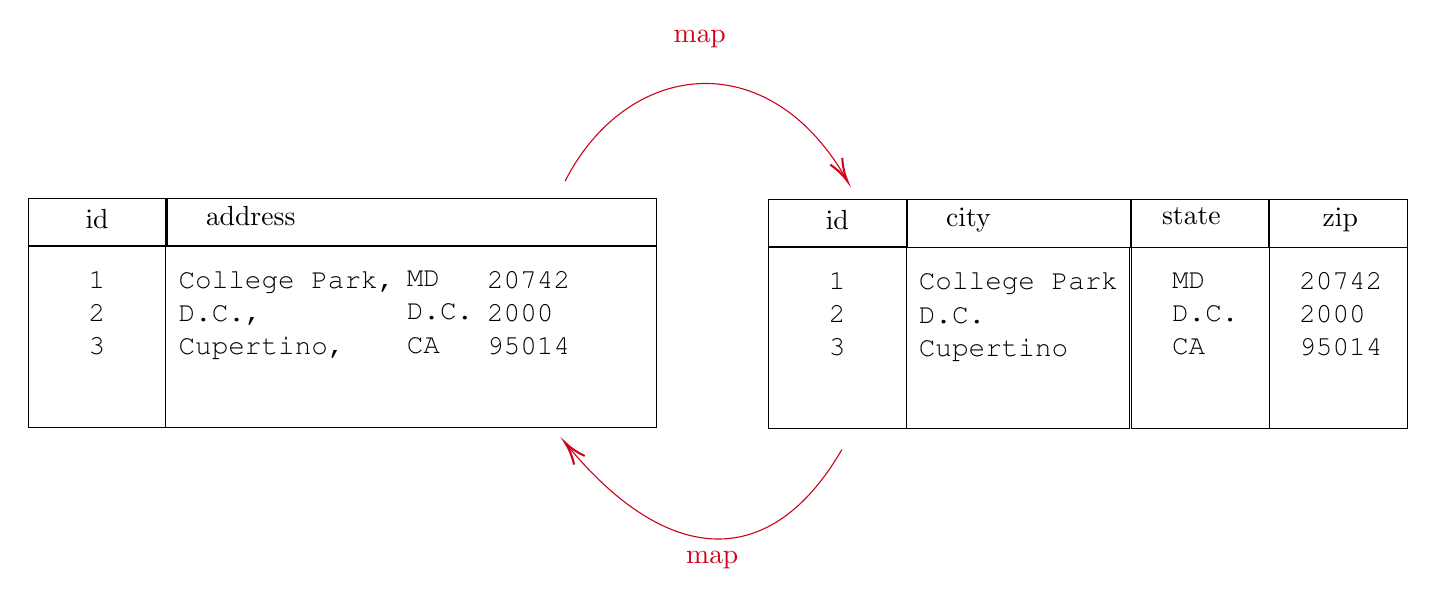
\begin{tikzpicture}[x=0.75pt,y=0.75pt,yscale=-1,xscale=1]
%uncomment if require: \path (0,300); %set diagram left start at 0, and has height of 300

%Shape: Rectangle [id:dp4887463946097159] 
\draw  [color={rgb, 255:red, 0; green, 0; blue, 0 }  ,draw opacity=1 ] (362.33,88.33) -- (428.67,88.33) -- (428.67,111.33) -- (362.33,111.33) -- cycle ;
%Shape: Rectangle [id:dp5770783881644757] 
\draw  [color={rgb, 255:red, 0; green, 0; blue, 0 }  ,draw opacity=1 ] (429.21,88.33) -- (537,88.33) -- (537,111.33) -- (429.21,111.33) -- cycle ;
%Shape: Rectangle [id:dp6134551110117208] 
\draw   (537,88.33) -- (603.33,88.33) -- (603.33,111.33) -- (537,111.33) -- cycle ;
%Shape: Rectangle [id:dp5531077995700737] 
\draw   (603.67,88.33) -- (670,88.33) -- (670,111.33) -- (603.67,111.33) -- cycle ;
%Shape: Rectangle [id:dp3313757499092773] 
\draw  [color={rgb, 255:red, 0; green, 0; blue, 0 }  ,draw opacity=1 ] (362.33,111) -- (428.67,111) -- (428.67,198.67) -- (362.33,198.67) -- cycle ;
%Shape: Rectangle [id:dp9339502110856537] 
\draw  [color={rgb, 255:red, 0; green, 0; blue, 0 }  ,draw opacity=1 ] (428.67,111.26) -- (536.46,111.26) -- (536.46,198.67) -- (428.67,198.67) -- cycle ;
%Shape: Rectangle [id:dp07892533389980638] 
\draw   (537.33,111.26) -- (603.67,111.26) -- (603.67,198.67) -- (537.33,198.67) -- cycle ;
%Shape: Rectangle [id:dp979611278461765] 
\draw   (603.67,111.26) -- (670,111.26) -- (670,198.67) -- (603.67,198.67) -- cycle ;
%Shape: Rectangle [id:dp717440949324254] 
\draw  [color={rgb, 255:red, 0; green, 0; blue, 0 }  ,draw opacity=1 ] (5.67,87.67) -- (72,87.67) -- (72,110.67) -- (5.67,110.67) -- cycle ;
%Shape: Rectangle [id:dp5659022269665408] 
\draw  [color={rgb, 255:red, 0; green, 0; blue, 0 }  ,draw opacity=1 ] (72.54,87.67) -- (308.33,87.67) -- (308.33,110.67) -- (72.54,110.67) -- cycle ;
%Shape: Rectangle [id:dp9470998578275607] 
\draw  [color={rgb, 255:red, 0; green, 0; blue, 0 }  ,draw opacity=1 ] (5.67,110.33) -- (72,110.33) -- (72,198) -- (5.67,198) -- cycle ;
%Shape: Rectangle [id:dp5421589353414771] 
\draw  [color={rgb, 255:red, 0; green, 0; blue, 0 }  ,draw opacity=1 ] (72,110.6) -- (308.33,110.6) -- (308.33,198) -- (72,198) -- cycle ;
%Curve Lines [id:da1781160675260307] 
\draw [color={rgb, 255:red, 208; green, 2; blue, 27 }  ,draw opacity=1 ]   (264.33,79.33) .. controls (294.18,20.96) and (362.31,12.75) .. (399.77,78.34) ;
\draw [shift={(400.33,79.33)}, rotate = 240.75] [color={rgb, 255:red, 208; green, 2; blue, 27 }  ,draw opacity=1 ][line width=0.75]    (10.93,-3.29) .. controls (6.95,-1.4) and (3.31,-0.3) .. (0,0) .. controls (3.31,0.3) and (6.95,1.4) .. (10.93,3.29)   ;
%Curve Lines [id:da028217104849822316] 
\draw [color={rgb, 255:red, 208; green, 2; blue, 27 }  ,draw opacity=1 ]   (397.67,208.67) .. controls (363.84,267.04) and (314.17,266.01) .. (265.07,206.24) ;
\draw [shift={(264.33,205.33)}, rotate = 410.88] [color={rgb, 255:red, 208; green, 2; blue, 27 }  ,draw opacity=1 ][line width=0.75]    (10.93,-3.29) .. controls (6.95,-1.4) and (3.31,-0.3) .. (0,0) .. controls (3.31,0.3) and (6.95,1.4) .. (10.93,3.29)   ;

% Text Node
\draw (388.67,92.33) node [anchor=north west][inner sep=0.75pt]   [align=left] {id};
% Text Node
\draw (390.17,122.06) node [anchor=north west][inner sep=0.75pt]   [align=left] {{\fontfamily{pcr}\selectfont 1}\\{\fontfamily{pcr}\selectfont 2}\\{\fontfamily{pcr}\selectfont 3}};
% Text Node
\draw (446.67,91) node [anchor=north west][inner sep=0.75pt]   [align=left] {city};
% Text Node
\draw (550.67,91) node [anchor=north west][inner sep=0.75pt]   [align=left] {state};
% Text Node
\draw (628,91) node [anchor=north west][inner sep=0.75pt]   [align=left] {zip};
% Text Node
\draw (433.5,122.06) node [anchor=north west][inner sep=0.75pt]   [align=left] {{\fontfamily{pcr}\selectfont College Park}\\{\fontfamily{pcr}\selectfont D.C.}\\{\fontfamily{pcr}\selectfont Cupertino}};
% Text Node
\draw (555.5,122.06) node [anchor=north west][inner sep=0.75pt]   [align=left] {{\fontfamily{pcr}\selectfont MD}\\{\fontfamily{pcr}\selectfont D.C.}\\{\fontfamily{pcr}\selectfont CA}};
% Text Node
\draw (616.83,122.06) node [anchor=north west][inner sep=0.75pt]   [align=left] {{\fontfamily{pcr}\selectfont 20742}\\{\fontfamily{pcr}\selectfont 2000}\\{\fontfamily{pcr}\selectfont 95014}};
% Text Node
\draw (32,91.67) node [anchor=north west][inner sep=0.75pt]   [align=left] {id};
% Text Node
\draw (33.5,121.39) node [anchor=north west][inner sep=0.75pt]   [align=left] {{\fontfamily{pcr}\selectfont 1}\\{\fontfamily{pcr}\selectfont 2}\\{\fontfamily{pcr}\selectfont 3}};
% Text Node
\draw (90,90.33) node [anchor=north west][inner sep=0.75pt]   [align=left] {address};
% Text Node
\draw (76.83,121.39) node [anchor=north west][inner sep=0.75pt]   [align=left] {{\fontfamily{pcr}\selectfont College Park,}\\{\fontfamily{pcr}\selectfont D.C., }\\{\fontfamily{pcr}\selectfont Cupertino, }};
% Text Node
\draw (186.83,121.39) node [anchor=north west][inner sep=0.75pt]   [align=left] {{\fontfamily{pcr}\selectfont MD}\\{\fontfamily{pcr}\selectfont D.C.}\\{\fontfamily{pcr}\selectfont CA}};
% Text Node
\draw (225.5,121.39) node [anchor=north west][inner sep=0.75pt]   [align=left] {{\fontfamily{pcr}\selectfont 20742}\\{\fontfamily{pcr}\selectfont 2000}\\{\fontfamily{pcr}\selectfont 95014}};
% Text Node
\draw (315.33,5.67) node [anchor=north west][inner sep=0.75pt]   [align=left] {\textcolor[rgb]{0.82,0.01,0.11}{map}};
% Text Node
\draw (321.33,256.33) node [anchor=north west][inner sep=0.75pt]   [align=left] {\textcolor[rgb]{0.82,0.01,0.11}{map}};


\end{tikzpicture}

}

\hfill \break Notice how applying map to either table is valid in this case- sometimes we want to break down columns into more specific values, and sometimes we want to combine them into singular columns. Each of these operations is totally valid, and has its uses. (This is evident in the projects for this class).\\

Again, this is mostly about what you need. There's no necessary better or worse in this case (more columns does not always equal better data).

\subsubsection{Group By}

Group By is an operation that allows you to group tuples together based on the values in columns/dimensions. Let's say we had the following table of house addresses like earlier. This time, we'll add the number of people in each house as a column as well.\\

{
\centering



\tikzset{every picture/.style={line width=0.75pt}} %set default line width to 0.75pt        

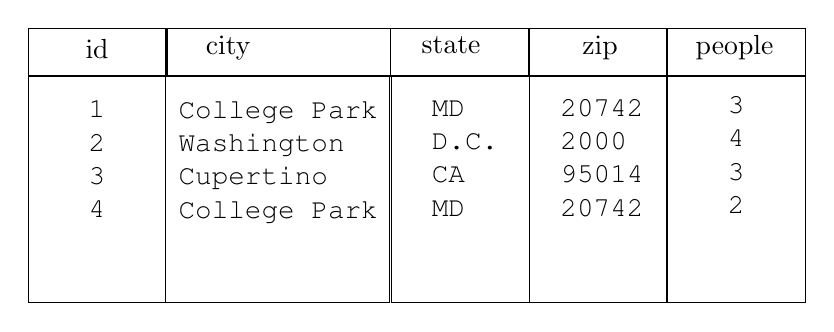
\begin{tikzpicture}[x=0.75pt,y=0.75pt,yscale=-1,xscale=1]
%uncomment if require: \path (0,300); %set diagram left start at 0, and has height of 300

%Shape: Rectangle [id:dp816510738764739] 
\draw  [color={rgb, 255:red, 0; green, 0; blue, 0 }  ,draw opacity=1 ] (185,62.33) -- (251.33,62.33) -- (251.33,85.33) -- (185,85.33) -- cycle ;
%Shape: Rectangle [id:dp39744801489204895] 
\draw  [color={rgb, 255:red, 0; green, 0; blue, 0 }  ,draw opacity=1 ] (251.87,62.33) -- (359.67,62.33) -- (359.67,85.33) -- (251.87,85.33) -- cycle ;
%Shape: Rectangle [id:dp16790194728351993] 
\draw   (359.67,62.33) -- (426,62.33) -- (426,85.33) -- (359.67,85.33) -- cycle ;
%Shape: Rectangle [id:dp5121628997613088] 
\draw   (426.33,62.33) -- (492.67,62.33) -- (492.67,85.33) -- (426.33,85.33) -- cycle ;
%Shape: Rectangle [id:dp38170728474734883] 
\draw  [color={rgb, 255:red, 0; green, 0; blue, 0 }  ,draw opacity=1 ] (185,85) -- (251.33,85) -- (251.33,194.67) -- (185,194.67) -- cycle ;
%Shape: Rectangle [id:dp0783518509199912] 
\draw  [color={rgb, 255:red, 0; green, 0; blue, 0 }  ,draw opacity=1 ] (251.33,85.33) -- (359.12,85.33) -- (359.12,194.67) -- (251.33,194.67) -- cycle ;
%Shape: Rectangle [id:dp8309347187193188] 
\draw   (360,85.33) -- (426.33,85.33) -- (426.33,194.67) -- (360,194.67) -- cycle ;
%Shape: Rectangle [id:dp0878616379496251] 
\draw   (426.33,85.33) -- (492.67,85.33) -- (492.67,194.67) -- (426.33,194.67) -- cycle ;
%Shape: Rectangle [id:dp9451653351898317] 
\draw   (493,62.33) -- (559.33,62.33) -- (559.33,85.33) -- (493,85.33) -- cycle ;
%Shape: Rectangle [id:dp11005059918565219] 
\draw   (493,85.33) -- (559.33,85.33) -- (559.33,194.67) -- (493,194.67) -- cycle ;

% Text Node
\draw (211.33,66.33) node [anchor=north west][inner sep=0.75pt]   [align=left] {id};
% Text Node
\draw (212.83,96.06) node [anchor=north west][inner sep=0.75pt]   [align=left] {{\fontfamily{pcr}\selectfont 1}\\{\fontfamily{pcr}\selectfont 2}\\{\fontfamily{pcr}\selectfont 3}\\{\fontfamily{pcr}\selectfont 4}\\};
% Text Node
\draw (269.33,65) node [anchor=north west][inner sep=0.75pt]   [align=left] {city};
% Text Node
\draw (373.33,65) node [anchor=north west][inner sep=0.75pt]   [align=left] {state};
% Text Node
\draw (450.67,65) node [anchor=north west][inner sep=0.75pt]   [align=left] {zip};
% Text Node
\draw (256.17,96.06) node [anchor=north west][inner sep=0.75pt]   [align=left] {{\fontfamily{pcr}\selectfont College Park}\\{\fontfamily{pcr}\selectfont Washington}\\{\fontfamily{pcr}\selectfont Cupertino}\\{\fontfamily{pcr}\selectfont College Park}};
% Text Node
\draw (378.17,96.06) node [anchor=north west][inner sep=0.75pt]   [align=left] {{\fontfamily{pcr}\selectfont MD}\\{\fontfamily{pcr}\selectfont D.C.}\\{\fontfamily{pcr}\selectfont CA}\\{\fontfamily{pcr}\selectfont MD}};
% Text Node
\draw (440.17,95.39) node [anchor=north west][inner sep=0.75pt]   [align=left] {{\fontfamily{pcr}\selectfont 20742}\\{\fontfamily{pcr}\selectfont 2000}\\{\fontfamily{pcr}\selectfont 95014}\\{\fontfamily{pcr}\selectfont 20742}};
% Text Node
\draw (505.33,64.33) node [anchor=north west][inner sep=0.75pt]   [align=left] {people};
% Text Node
\draw (520.83,94.06) node [anchor=north west][inner sep=0.75pt]   [align=left] {{\fontfamily{pcr}\selectfont 3}\\{\fontfamily{pcr}\selectfont 4}\\{\fontfamily{pcr}\selectfont 3}\\{\fontfamily{pcr}\selectfont 2}};


\end{tikzpicture}

}

Let's say we only wanted to see the data from a \textbf{single city}. In this case, let's pick College Park.\newline

{
\centering



\tikzset{every picture/.style={line width=0.75pt}} %set default line width to 0.75pt        

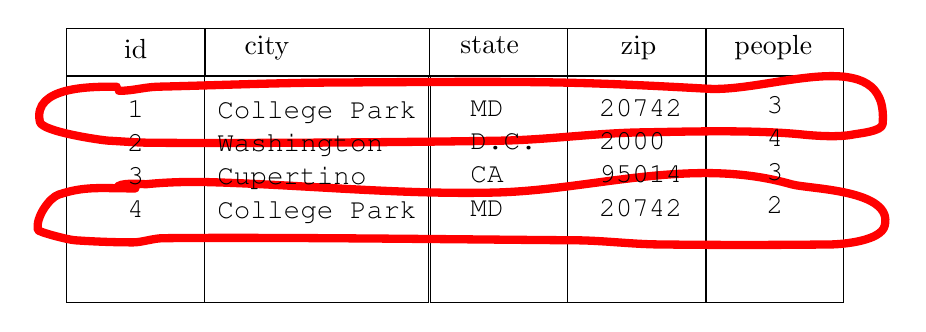
\begin{tikzpicture}[x=0.75pt,y=0.75pt,yscale=-1,xscale=1]
%uncomment if require: \path (0,300); %set diagram left start at 0, and has height of 300

%Shape: Rectangle [id:dp816510738764739] 
\draw  [color={rgb, 255:red, 0; green, 0; blue, 0 }  ,draw opacity=1 ] (185,62.33) -- (251.33,62.33) -- (251.33,85.33) -- (185,85.33) -- cycle ;
%Shape: Rectangle [id:dp39744801489204895] 
\draw  [color={rgb, 255:red, 0; green, 0; blue, 0 }  ,draw opacity=1 ] (251.87,62.33) -- (359.67,62.33) -- (359.67,85.33) -- (251.87,85.33) -- cycle ;
%Shape: Rectangle [id:dp16790194728351993] 
\draw   (359.67,62.33) -- (426,62.33) -- (426,85.33) -- (359.67,85.33) -- cycle ;
%Shape: Rectangle [id:dp5121628997613088] 
\draw   (426.33,62.33) -- (492.67,62.33) -- (492.67,85.33) -- (426.33,85.33) -- cycle ;
%Shape: Rectangle [id:dp38170728474734883] 
\draw  [color={rgb, 255:red, 0; green, 0; blue, 0 }  ,draw opacity=1 ] (185,85) -- (251.33,85) -- (251.33,194.67) -- (185,194.67) -- cycle ;
%Shape: Rectangle [id:dp0783518509199912] 
\draw  [color={rgb, 255:red, 0; green, 0; blue, 0 }  ,draw opacity=1 ] (251.33,85.33) -- (359.12,85.33) -- (359.12,194.67) -- (251.33,194.67) -- cycle ;
%Shape: Rectangle [id:dp8309347187193188] 
\draw   (360,85.33) -- (426.33,85.33) -- (426.33,194.67) -- (360,194.67) -- cycle ;
%Shape: Rectangle [id:dp0878616379496251] 
\draw   (426.33,85.33) -- (492.67,85.33) -- (492.67,194.67) -- (426.33,194.67) -- cycle ;
%Shape: Rectangle [id:dp9451653351898317] 
\draw   (493,62.33) -- (559.33,62.33) -- (559.33,85.33) -- (493,85.33) -- cycle ;
%Shape: Rectangle [id:dp11005059918565219] 
\draw   (493,85.33) -- (559.33,85.33) -- (559.33,194.67) -- (493,194.67) -- cycle ;
%Shape: Free Drawing [id:dp983490163154191] 
\draw  [color={rgb, 255:red, 255; green, 0; blue, 0 }  ,draw opacity=1 ][line width=3] [line join = round][line cap = round] (209,90.5) .. controls (198.12,90.5) and (168.09,89.91) .. (172,107.5) .. controls (173.05,112.21) and (201.95,116.35) .. (205,116.5) .. controls (211.67,116.83) and (218.33,117.44) .. (225,117.5) .. controls (265.32,117.85) and (345.68,117.33) .. (394,116.5) .. controls (416.57,116.11) and (439.52,112.83) .. (462,112.5) .. controls (480.28,112.24) and (514.78,111.08) .. (539,113.5) .. controls (546.8,114.28) and (556.96,114.91) .. (564,113.5) .. controls (566.72,112.96) and (577.71,112.02) .. (578,108.5) .. controls (581.35,68.27) and (524.35,93.19) .. (494,91.5) .. controls (427.64,87.81) and (413.09,87.87) .. (312,88.5) .. controls (284.83,88.67) and (256.23,89.85) .. (229,90.5) .. controls (222.28,90.66) and (216.95,92.5) .. (210,92.5) ;
%Curve Lines [id:da10861026576502275] 
\draw [color={rgb, 255:red, 255; green, 0; blue, 0 }  ,draw opacity=1 ][line width=3] [line join = round][line cap = round]   (218,139.5) .. controls (201.04,139.5) and (193.69,138.27) .. (181,142.5) .. controls (176.53,143.99) and (169.8,153.48) .. (171,159.5) .. controls (171.2,160.48) and (185.36,164.26) .. (189,164.5) .. controls (198.32,165.12) and (207.66,165.5) .. (217,165.5) .. controls (221.09,165.5) and (226.66,163.55) .. (231,163.5) .. controls (282.82,162.87) and (384.95,164.21) .. (430,164.5) .. controls (443.35,164.59) and (456.65,166.35) .. (470,166.5) .. controls (497.66,166.82) and (525.34,166.82) .. (553,166.5) .. controls (558.97,166.43) and (577.17,164.8) .. (579,157.5) .. controls (583.4,139.91) and (542.58,139.95) .. (534,137.5) .. controls (486.11,123.82) and (438.47,140.4) .. (391,141.5) .. controls (345.12,142.57) and (299.53,137.8) .. (254,136.5) .. controls (243.67,136.2) and (233.29,136.47) .. (223,137.5) .. controls (222.9,137.51) and (209,136.14) .. (209,139.5) ;

% Text Node
\draw (211.33,66.33) node [anchor=north west][inner sep=0.75pt]   [align=left] {id};
% Text Node
\draw (212.83,96.06) node [anchor=north west][inner sep=0.75pt]   [align=left] {{\fontfamily{pcr}\selectfont 1}\\{\fontfamily{pcr}\selectfont 2}\\{\fontfamily{pcr}\selectfont 3}\\{\fontfamily{pcr}\selectfont 4}\\};
% Text Node
\draw (269.33,65) node [anchor=north west][inner sep=0.75pt]   [align=left] {city};
% Text Node
\draw (373.33,65) node [anchor=north west][inner sep=0.75pt]   [align=left] {state};
% Text Node
\draw (450.67,65) node [anchor=north west][inner sep=0.75pt]   [align=left] {zip};
% Text Node
\draw (256.17,96.06) node [anchor=north west][inner sep=0.75pt]   [align=left] {{\fontfamily{pcr}\selectfont College Park}\\{\fontfamily{pcr}\selectfont Washington}\\{\fontfamily{pcr}\selectfont Cupertino}\\{\fontfamily{pcr}\selectfont College Park}};
% Text Node
\draw (378.17,96.06) node [anchor=north west][inner sep=0.75pt]   [align=left] {{\fontfamily{pcr}\selectfont MD}\\{\fontfamily{pcr}\selectfont D.C.}\\{\fontfamily{pcr}\selectfont CA}\\{\fontfamily{pcr}\selectfont MD}};
% Text Node
\draw (440.17,95.39) node [anchor=north west][inner sep=0.75pt]   [align=left] {{\fontfamily{pcr}\selectfont 20742}\\{\fontfamily{pcr}\selectfont 2000}\\{\fontfamily{pcr}\selectfont 95014}\\{\fontfamily{pcr}\selectfont 20742}};
% Text Node
\draw (505.33,64.33) node [anchor=north west][inner sep=0.75pt]   [align=left] {people};
% Text Node
\draw (520.83,94.06) node [anchor=north west][inner sep=0.75pt]   [align=left] {{\fontfamily{pcr}\selectfont 3}\\{\fontfamily{pcr}\selectfont 4}\\{\fontfamily{pcr}\selectfont 3}\\{\fontfamily{pcr}\selectfont 2}};


\end{tikzpicture}

}

This is what a 'Group By' operation would be perfect for. It'll basically just get us the rows that are from the city that we want.

\subsubsection{Group By + Aggregate}

We can combined Group By and Aggregate in pretty cool ways to get results that we want. For example, let's say we wanted to leverage the above table and get the sum total of all people who live in College Park, D.C., and Cupertino, respectively. By using a combo of Group By and Aggregate, we can totally do that. (\textit{Group By} City, then perform summing \textit{aggregation} operation.)

\subsubsection{Union, Intersection, Difference}

These are your usual set operations from statistics. However, this only works if the tables have identical attributes (columns). If they have identical columns, they are called \textbf{compatible tables}.\\

Examples: (Table A) $\union$ (Table B) results in (Table C) where all three tables have the same attributes. Likewise, (Table A) $\cap$ (Table B) results in (Table D) where all three also have the same attributes.

\subsubsection{Merge or Join}

This is how you combine rows across tables, based on some distinguishing element (i.e. ID column). For example, you'd basically take the row with ID 1 in your first table and add all those elements to the row with ID 1 in your second table.\\

There isn't a graphical example here just because we'll be talking about this a lot more in depth in later lectures. For now, just remember it as a way to combine tables.

\subsubsection{Summary}

Overall, \textbf{Tables} are a simple and common abstraction. They're how we mainly keep track of data when we do most of these data science things, so it's worth learning how to employ them, and what basic operations we can use when manipulating them.\\

These \textbf{operations}, at a glance:

\begin{itemize}
	\item Select
	\item Map
	\item Aggregate/Reduce
	\item Join/Merge
	\item Union/Concat
	\item Group By
\end{itemize} 

Keep in mind that tables are an \textit{abstraction}, after all, so these operations may be named different things in the languages you use to manipulate them. That's why its important to not just memorize the names of these operations, but what they actually do. This will prepare you for work with any data table manipulation program.

\subsection{Pandas}

\texttt{PANDAS} is a data manipulation library for Python that's highly optimized for performance. It contains two key constructs, \textbf{\texttt{Dataframes}} and \textbf{\texttt{Series}}.

\subsubsection{Dataframes}

This is \texttt{PANDAS}'s way of representing the table abstraction we were looking at. Geeksforgeeks even calls this one a tabular data structure.\\

There are a lot of \texttt{PANDAS}-specific commands that you'll have to learn to be proficient with these, but Geeksforgeeks is a great reference for them. (You'll find it's pretty easy to conduct all the basic table operations)\\

{
\centering

\tikzset{every picture/.style={line width=0.75pt}} %set default line width to 0.75pt        

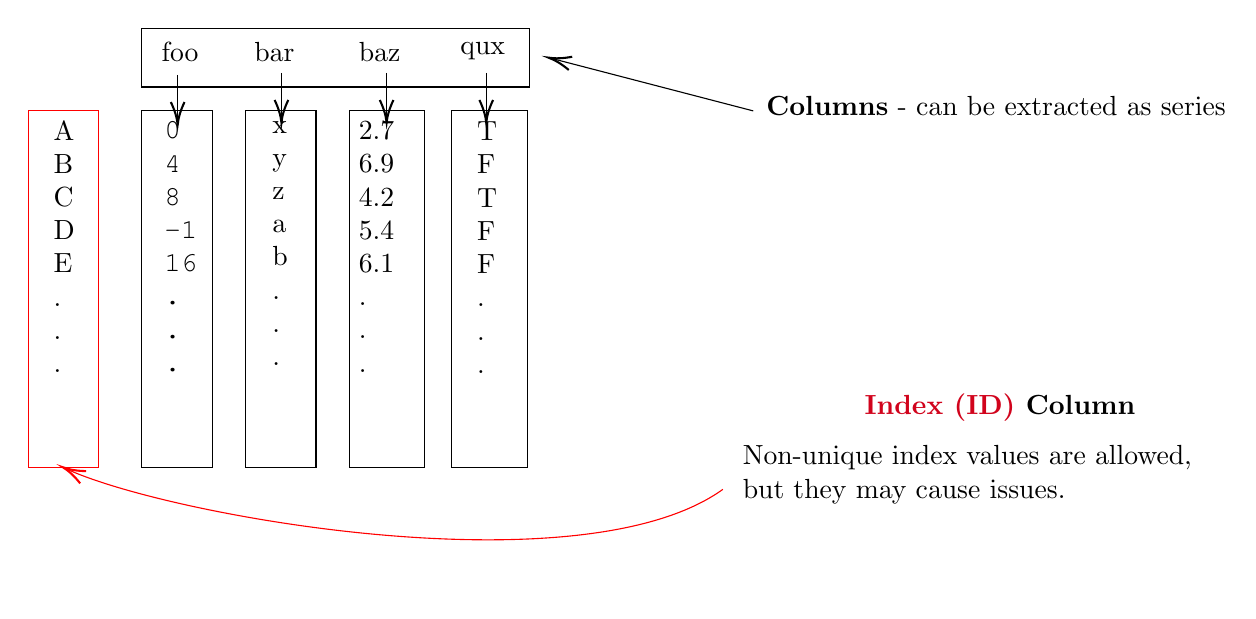
\begin{tikzpicture}[x=0.75pt,y=0.75pt,yscale=-1,xscale=1]
%uncomment if require: \path (0,300); %set diagram left start at 0, and has height of 300

%Shape: Rectangle [id:dp2777454383178828] 
\draw   (109.67,31.83) -- (296.33,31.83) -- (296.33,60.17) -- (109.67,60.17) -- cycle ;
%Shape: Rectangle [id:dp24695275768955183] 
\draw   (109.67,71.67) -- (143.67,71.67) -- (143.67,243.33) -- (109.67,243.33) -- cycle ;
%Shape: Rectangle [id:dp32304758523801747] 
\draw   (159.67,71.67) -- (193.67,71.67) -- (193.67,243.33) -- (159.67,243.33) -- cycle ;
%Shape: Rectangle [id:dp3982940173231615] 
\draw   (210,71.67) -- (246,71.67) -- (246,243.33) -- (210,243.33) -- cycle ;
%Shape: Rectangle [id:dp37628168334169354] 
\draw   (259,71.67) -- (295.67,71.67) -- (295.67,243.33) -- (259,243.33) -- cycle ;
%Straight Lines [id:da7379961166553421] 
\draw    (127,54.33) -- (127,76.33) ;
\draw [shift={(127,78.33)}, rotate = 270] [color={rgb, 255:red, 0; green, 0; blue, 0 }  ][line width=0.75]    (10.93,-3.29) .. controls (6.95,-1.4) and (3.31,-0.3) .. (0,0) .. controls (3.31,0.3) and (6.95,1.4) .. (10.93,3.29)   ;
%Straight Lines [id:da8157307687769006] 
\draw    (177,53.33) -- (177,75.33) ;
\draw [shift={(177,77.33)}, rotate = 270] [color={rgb, 255:red, 0; green, 0; blue, 0 }  ][line width=0.75]    (10.93,-3.29) .. controls (6.95,-1.4) and (3.31,-0.3) .. (0,0) .. controls (3.31,0.3) and (6.95,1.4) .. (10.93,3.29)   ;
%Straight Lines [id:da85290367528958] 
\draw    (227.67,53.33) -- (227.67,75.33) ;
\draw [shift={(227.67,77.33)}, rotate = 270] [color={rgb, 255:red, 0; green, 0; blue, 0 }  ][line width=0.75]    (10.93,-3.29) .. controls (6.95,-1.4) and (3.31,-0.3) .. (0,0) .. controls (3.31,0.3) and (6.95,1.4) .. (10.93,3.29)   ;
%Straight Lines [id:da06750596708048917] 
\draw    (275.67,53.33) -- (275.67,75.33) ;
\draw [shift={(275.67,77.33)}, rotate = 270] [color={rgb, 255:red, 0; green, 0; blue, 0 }  ][line width=0.75]    (10.93,-3.29) .. controls (6.95,-1.4) and (3.31,-0.3) .. (0,0) .. controls (3.31,0.3) and (6.95,1.4) .. (10.93,3.29)   ;
%Shape: Rectangle [id:dp30009607301124297] 
\draw  [color={rgb, 255:red, 255; green, 0; blue, 0 }  ,draw opacity=1 ] (55,71.67) -- (89,71.67) -- (89,243.33) -- (55,243.33) -- cycle ;
%Curve Lines [id:da3683895080925861] 
\draw [color={rgb, 255:red, 255; green, 0; blue, 0 }  ,draw opacity=1 ]   (389.67,254) .. controls (321.69,302.84) and (121.72,266.74) .. (73.09,244.02) ;
\draw [shift={(71.67,243.33)}, rotate = 386.23] [color={rgb, 255:red, 255; green, 0; blue, 0 }  ,draw opacity=1 ][line width=0.75]    (10.93,-3.29) .. controls (6.95,-1.4) and (3.31,-0.3) .. (0,0) .. controls (3.31,0.3) and (6.95,1.4) .. (10.93,3.29)   ;
%Straight Lines [id:da5179190869487518] 
\draw    (404.33,71.67) -- (307.6,46.5) ;
\draw [shift={(305.67,46)}, rotate = 374.58000000000004] [color={rgb, 255:red, 0; green, 0; blue, 0 }  ][line width=0.75]    (10.93,-3.29) .. controls (6.95,-1.4) and (3.31,-0.3) .. (0,0) .. controls (3.31,0.3) and (6.95,1.4) .. (10.93,3.29)   ;

% Text Node
\draw (118,37.5) node [anchor=north west][inner sep=0.75pt]   [align=left] {foo};
% Text Node
\draw (162.67,37.5) node [anchor=north west][inner sep=0.75pt]   [align=left] {bar};
% Text Node
\draw (213,37.5) node [anchor=north west][inner sep=0.75pt]   [align=left] {baz};
% Text Node
\draw (262,37.5) node [anchor=north west][inner sep=0.75pt]   [align=left] {qux};
% Text Node
\draw (66,75.33) node [anchor=north west][inner sep=0.75pt]   [align=left] {A\\B\\C\\D\\E\\.\\.\\.};
% Text Node
\draw (119.33,75.67) node [anchor=north west][inner sep=0.75pt]   [align=left] {{\fontfamily{pcr}\selectfont 0}\\{\fontfamily{pcr}\selectfont 4}\\{\fontfamily{pcr}\selectfont 8}\\{\fontfamily{pcr}\selectfont -1}\\{\fontfamily{pcr}\selectfont 16}\\{\fontfamily{pcr}\selectfont .}\\{\fontfamily{pcr}\selectfont .}\\{\fontfamily{pcr}\selectfont .}};
% Text Node
\draw (171.33,75.33) node [anchor=north west][inner sep=0.75pt]   [align=left] {x\\y\\z\\a\\b\\.\\.\\.};
% Text Node
\draw (213,75.67) node [anchor=north west][inner sep=0.75pt]   [align=left] {2.7\\6.9\\4.2\\5.4\\6.1\\.\\.\\.};
% Text Node
\draw (270,75.67) node [anchor=north west][inner sep=0.75pt]   [align=left] {T\\F\\T\\F\\F\\.\\.\\.};
% Text Node
\draw (398,231.67) node [anchor=north west][inner sep=0.75pt]   [align=left] {Non-unique index values are allowed,\\ but they may cause issues.};
% Text Node
\draw (456.67,206.67) node [anchor=north west][inner sep=0.75pt]   [align=left] {\textbf{\textcolor[rgb]{0.82,0.01,0.11}{Index (ID)} Column}};
% Text Node
\draw (409.33,63.17) node [anchor=north west][inner sep=0.75pt]   [align=left] {\textbf{Columns} - can be extracted as series};


\end{tikzpicture}

}


\subsubsection{Series}

Think of a \texttt{series} as a subclass of Numpy's \texttt{ndarray}.\\

Geeksforgeeks calls this a 'one dimensional labeled array capable of holding any data type'. Think of it as a column in an Excel spreadsheet. In fact, their most common use is when you pull a single column out of a \texttt{dataframe} and want to analyze it individually.\\

The object itself supports integer and label based indexing (like letters), and allows us to perform a bunch of operations involving the index.\\

To create one of these we can grab a column from a \texttt{dataframe}, or we can create one out of a regular Python \texttt{list} or a Numpy  \texttt{ndarray}.

{
\centering



\tikzset{every picture/.style={line width=0.75pt}} %set default line width to 0.75pt        

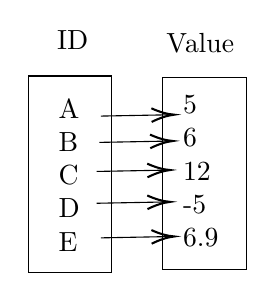
\begin{tikzpicture}[x=0.75pt,y=0.75pt,yscale=-1,xscale=1]
%uncomment if require: \path (0,300); %set diagram left start at 0, and has height of 300

%Shape: Rectangle [id:dp043234274585036925] 
\draw   (352.67,87.33) -- (393,87.33) -- (393,180) -- (352.67,180) -- cycle ;
%Shape: Rectangle [id:dp5031953197422854] 
\draw   (288,86.67) -- (328.33,86.67) -- (328.33,181.33) -- (288,181.33) -- cycle ;
%Straight Lines [id:da8511139241388785] 
\draw    (323,106) -- (356.33,105.37) ;
\draw [shift={(358.33,105.33)}, rotate = 538.9200000000001] [color={rgb, 255:red, 0; green, 0; blue, 0 }  ][line width=0.75]    (10.93,-3.29) .. controls (6.95,-1.4) and (3.31,-0.3) .. (0,0) .. controls (3.31,0.3) and (6.95,1.4) .. (10.93,3.29)   ;
%Straight Lines [id:da28107306227000595] 
\draw    (322.33,118.67) -- (355.67,118.04) ;
\draw [shift={(357.67,118)}, rotate = 538.9200000000001] [color={rgb, 255:red, 0; green, 0; blue, 0 }  ][line width=0.75]    (10.93,-3.29) .. controls (6.95,-1.4) and (3.31,-0.3) .. (0,0) .. controls (3.31,0.3) and (6.95,1.4) .. (10.93,3.29)   ;
%Straight Lines [id:da8988638709435195] 
\draw    (321,132.67) -- (354.33,132.04) ;
\draw [shift={(356.33,132)}, rotate = 538.9200000000001] [color={rgb, 255:red, 0; green, 0; blue, 0 }  ][line width=0.75]    (10.93,-3.29) .. controls (6.95,-1.4) and (3.31,-0.3) .. (0,0) .. controls (3.31,0.3) and (6.95,1.4) .. (10.93,3.29)   ;
%Straight Lines [id:da21706629371432573] 
\draw    (321,148) -- (354.33,147.37) ;
\draw [shift={(356.33,147.33)}, rotate = 538.9200000000001] [color={rgb, 255:red, 0; green, 0; blue, 0 }  ][line width=0.75]    (10.93,-3.29) .. controls (6.95,-1.4) and (3.31,-0.3) .. (0,0) .. controls (3.31,0.3) and (6.95,1.4) .. (10.93,3.29)   ;
%Straight Lines [id:da8917362815148493] 
\draw    (323,164.67) -- (356.33,164.04) ;
\draw [shift={(358.33,164)}, rotate = 538.9200000000001] [color={rgb, 255:red, 0; green, 0; blue, 0 }  ][line width=0.75]    (10.93,-3.29) .. controls (6.95,-1.4) and (3.31,-0.3) .. (0,0) .. controls (3.31,0.3) and (6.95,1.4) .. (10.93,3.29)   ;

% Text Node
\draw (361.33,95) node [anchor=north west][inner sep=0.75pt]   [align=left] {5\\6\\12\\\mbox{-}5\\6.9};
% Text Node
\draw (301.33,96.67) node [anchor=north west][inner sep=0.75pt]   [align=left] {A\\B\\C\\D\\E};
% Text Node
\draw (300.67,63.67) node [anchor=north west][inner sep=0.75pt]   [align=left] {ID};
% Text Node
\draw (353.33,65) node [anchor=north west][inner sep=0.75pt]   [align=left] {Value};
\end{tikzpicture}


}

\hfill \break For this sort of stuff, you can probably look at \textbf{GeeksforGeeks} for more information. They have excellent documentation on \texttt{PANDAS} functionality.

\subsubsection{Creating a Dataframe}

To \textbf{create a \texttt{dataframe}}, you have a variety of options.

\begin{itemize}
	\item Get data directly from a Python dictionary, a bunch of series, or other data structures
	\item \texttt{Pandas.read\_csv()} $\rightarrow$ take in data from a \texttt{.csv} file
	\item \texttt{Pandas.read\_excel()} $\rightarrow$ take in data from an excel spreadsheet
	\item \texttt{Pandas.read\_html()} $\rightarrow$ take in data from a (static) website (e.g. a website with a big table of data on it)
	\item From a database by using SQL to make queries
	\item From clipboard, URL, many more options.
\end{itemize}

\subsection{Tidy Data}

There are \textbf{3} components of \textbf{tidy data}: \textbf{Labels},  \textbf{Variables} (values), and \textbf{Observations}.\\

{

\centering





\tikzset{every picture/.style={line width=0.75pt}} %set default line width to 0.75pt        

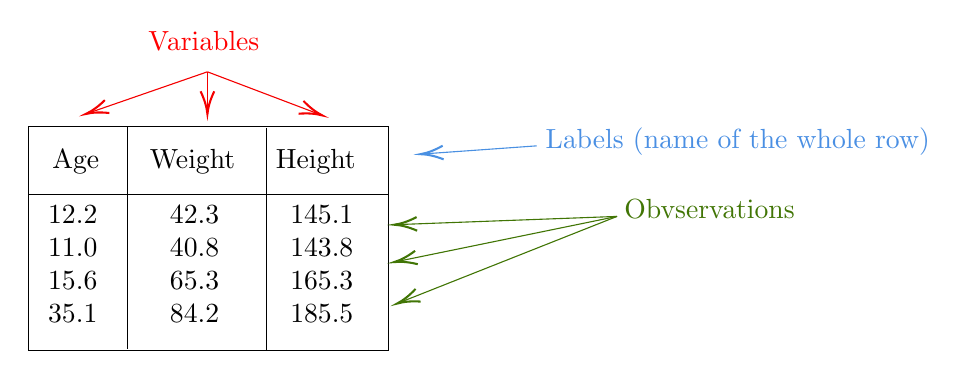
\begin{tikzpicture}[x=0.75pt,y=0.75pt,yscale=-1,xscale=1]
%uncomment if require: \path (0,300); %set diagram left start at 0, and has height of 300

%Shape: Rectangle [id:dp30513253458375056] 
\draw   (164,83.33) -- (337.67,83.33) -- (337.67,191.33) -- (164,191.33) -- cycle ;
%Straight Lines [id:da42703415044249615] 
\draw    (164,116) -- (337.67,116) ;
%Straight Lines [id:da4850478853225664] 
\draw    (211.67,83.33) -- (211.67,190.67) ;
%Straight Lines [id:da18466499361867394] 
\draw [color={rgb, 255:red, 244; green, 0; blue, 0 }  ,draw opacity=1 ]   (250.33,57) -- (193.56,76.68) ;
\draw [shift={(191.67,77.33)}, rotate = 340.88] [color={rgb, 255:red, 244; green, 0; blue, 0 }  ,draw opacity=1 ][line width=0.75]    (10.93,-3.29) .. controls (6.95,-1.4) and (3.31,-0.3) .. (0,0) .. controls (3.31,0.3) and (6.95,1.4) .. (10.93,3.29)   ;
%Straight Lines [id:da9858889971902263] 
\draw [color={rgb, 255:red, 244; green, 0; blue, 0 }  ,draw opacity=1 ]   (250.33,57) -- (250.33,75.33) ;
\draw [shift={(250.33,77.33)}, rotate = 270] [color={rgb, 255:red, 244; green, 0; blue, 0 }  ,draw opacity=1 ][line width=0.75]    (10.93,-3.29) .. controls (6.95,-1.4) and (3.31,-0.3) .. (0,0) .. controls (3.31,0.3) and (6.95,1.4) .. (10.93,3.29)   ;
%Straight Lines [id:da5731285595473614] 
\draw [color={rgb, 255:red, 244; green, 0; blue, 0 }  ,draw opacity=1 ]   (250.33,57) -- (303.8,77.29) ;
\draw [shift={(305.67,78)}, rotate = 200.78] [color={rgb, 255:red, 244; green, 0; blue, 0 }  ,draw opacity=1 ][line width=0.75]    (10.93,-3.29) .. controls (6.95,-1.4) and (3.31,-0.3) .. (0,0) .. controls (3.31,0.3) and (6.95,1.4) .. (10.93,3.29)   ;
%Straight Lines [id:da9175469839720249] 
\draw [color={rgb, 255:red, 74; green, 144; blue, 226 }  ,draw opacity=1 ]   (409,92.67) -- (354.99,96.52) ;
\draw [shift={(353,96.67)}, rotate = 355.90999999999997] [color={rgb, 255:red, 74; green, 144; blue, 226 }  ,draw opacity=1 ][line width=0.75]    (10.93,-3.29) .. controls (6.95,-1.4) and (3.31,-0.3) .. (0,0) .. controls (3.31,0.3) and (6.95,1.4) .. (10.93,3.29)   ;
%Straight Lines [id:da6295025530716172] 
\draw [color={rgb, 255:red, 65; green, 117; blue, 5 }  ,draw opacity=1 ]   (447.67,126.67) -- (342.33,130.59) ;
\draw [shift={(340.33,130.67)}, rotate = 357.87] [color={rgb, 255:red, 65; green, 117; blue, 5 }  ,draw opacity=1 ][line width=0.75]    (10.93,-3.29) .. controls (6.95,-1.4) and (3.31,-0.3) .. (0,0) .. controls (3.31,0.3) and (6.95,1.4) .. (10.93,3.29)   ;
%Straight Lines [id:da28024077694656935] 
\draw [color={rgb, 255:red, 65; green, 117; blue, 5 }  ,draw opacity=1 ]   (447.67,126.67) -- (342.29,148.27) ;
\draw [shift={(340.33,148.67)}, rotate = 348.41999999999996] [color={rgb, 255:red, 65; green, 117; blue, 5 }  ,draw opacity=1 ][line width=0.75]    (10.93,-3.29) .. controls (6.95,-1.4) and (3.31,-0.3) .. (0,0) .. controls (3.31,0.3) and (6.95,1.4) .. (10.93,3.29)   ;
%Straight Lines [id:da7161677482922817] 
\draw [color={rgb, 255:red, 65; green, 117; blue, 5 }  ,draw opacity=1 ]   (447.67,126.67) -- (343.53,167.93) ;
\draw [shift={(341.67,168.67)}, rotate = 338.39] [color={rgb, 255:red, 65; green, 117; blue, 5 }  ,draw opacity=1 ][line width=0.75]    (10.93,-3.29) .. controls (6.95,-1.4) and (3.31,-0.3) .. (0,0) .. controls (3.31,0.3) and (6.95,1.4) .. (10.93,3.29)   ;
%Straight Lines [id:da23343105546492038] 
\draw    (279,84) -- (279,191.33) ;

% Text Node
\draw (174.33,93) node [anchor=north west][inner sep=0.75pt]   [align=left] {Age};
% Text Node
\draw (221.33,93) node [anchor=north west][inner sep=0.75pt]   [align=left] {Weight};
% Text Node
\draw (282,93) node [anchor=north west][inner sep=0.75pt]   [align=left] {Height};
% Text Node
\draw (172.33,120) node [anchor=north west][inner sep=0.75pt]   [align=left] {12.2\\11.0\\15.6\\35.1};
% Text Node
\draw (231,120) node [anchor=north west][inner sep=0.75pt]   [align=left] {42.3\\40.8\\65.3\\84.2};
% Text Node
\draw (289,120) node [anchor=north west][inner sep=0.75pt]   [align=left] {145.1\\143.8\\165.3\\185.5};
% Text Node
\draw (220.67,36) node [anchor=north west][inner sep=0.75pt]   [align=left] {\textcolor[rgb]{1,0,0}{Variables}};
% Text Node
\draw (412,82.67) node [anchor=north west][inner sep=0.75pt]   [align=left] {\textcolor[rgb]{0.29,0.56,0.89}{Labels (name of the whole row)}};
% Text Node
\draw (450,117.33) node [anchor=north west][inner sep=0.75pt]  [color={rgb, 255:red, 65; green, 117; blue, 5 }  ,opacity=1 ] [align=left] {Obvservations};


\end{tikzpicture}

}

\hfill \break Here's some elaboration.

\begin{itemize}
	\item \textbf{Variables} $\rightarrow$ A measure or attribute, e.g. age, weight, height, sex.
	\item \textbf{Value} $\rightarrow$ Measurement of a \textit{singular} attribute, e.g. \texttt{12.2 lbs} or \texttt{5.9 inches}.
	\item \textbf{Observation} $\rightarrow$ All measurements for an object; a \textit{row} in the table. E.g. a single observation in the above table would be \texttt{[12.2, 42.3, 145.1]}.
\end{itemize}

Tidying and melting data basically just means that you mix data around until it's nice and usable. Usually, you are tidying in pursuit of a specific use-case, so less columns or more columns are never the 'better' option. This is one of those things that takes practice and application.\\

\textbf{TL;DR} Clean up and organize your data before you mess with it!

\subsection{SQL and Relational Databases}

\textbf{Big Question:} What is a relation?\\
\textbf{Answer:} In a databases context, they usually mean, "a tabular set of data either permanently stored in the database (a table) or derived from tables according to a mathematical description (a view or a query result)." (\textit{Larry Lustig, Stackoverflow})\\

\begin{tcolorbox}[title=Definition:,colframe=red!75!black,colback=red!5!white,arc=0pt,fonttitle=\bfseries]
\textbf{Relation} $\rightarrow$ A relation is a data structure which consists of a heading and an unordered set of tuples which share the same type.\\
\textbf{Relation Schema} $\rightarrow$ A list of all attribute names and their domains. E.g. 'The Schema for a Table'.
\end{tcolorbox}

\subsubsection{Indexing}

\begin{tcolorbox}[title=Definition:,colframe=red!75!black,colback=red!5!white,arc=0pt,fonttitle=\bfseries]
\textbf{Index} $\rightarrow$ An auxiliary data structure of a relation database designed to speed up the retrieval of rows.
\end{tcolorbox}


\hfill \break How can we leverage \textbf{indexes} to improve search times for our relational databases? Take a look at the example below. Let's say we wanted to find all people from Canada (with a nat\_id of 2).\\

{
\centering

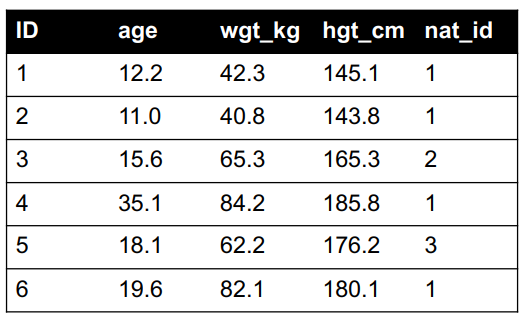
\includegraphics[scale=0.35]{img/table_1.png} 

}

\hfill \break Unfortunately, the time it takes for us to build this list every time we want to leverage the result of this search is \texttt{\textbf{O(n)}}. This is not so great for us. However, if we decide to build an \textbf{index} on the 'nat\_id' attribute, things change. \\

{
\centering

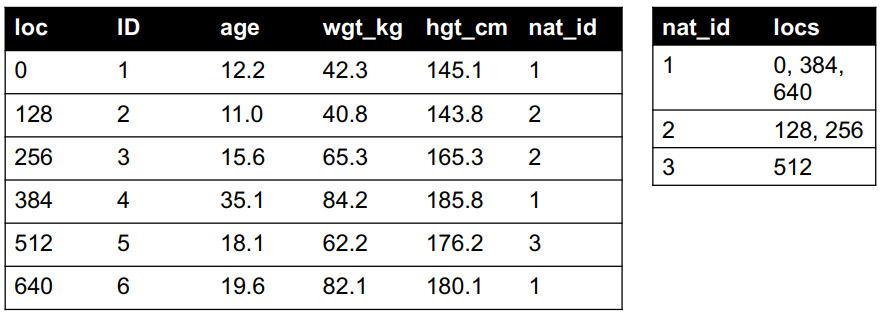
\includegraphics[scale=0.35]{img/table_2.png} 

}


\hfill \break Now, after establishing this index, which acts like a hidden sorted map of references to a specific attribute in a table, we are allowed \texttt{\textbf{O(log n)}} lookup with the parameter nat\_id.\\

You can choose to build an index on a certain attribute to improve search times for it, but they aren't free. They're expensive- establish an index with caution. Not only do they take time to initially build, but now, whenever you add to the table or update it, you also need to update the index. In that sense, establishing too many indexes could lead to other operations, such as changing table values, taking a very long time. It's a delicate balance.\\


\begin{tcolorbox}[title=Aside: Indexes,colframe=black,colback=white,arc=0pt,fonttitle=\bfseries]
Indexes are actually implemented with data structures like \textbf{B-trees}, which is why we are able to perform data access in \texttt{O(log n)} time. The worst case height of a B-tree is \texttt{O(log n)}, and since a search is dependent on height, B-tree lookups run in \texttt{O(log n)} on average.
\end{tcolorbox}


\subsection{Relationships}

Primary keys and foreign keys determine interactions between different tables. These are formally known as relationships. First, let's establish definitions for primary and foreign keys.\\

\begin{tcolorbox}[title=Definition:,colframe=red!75!black,colback=red!5!white,arc=0pt,fonttitle=\bfseries]
\textbf{Primary Keys} $\rightarrow$ Columns whose data can be used to uniquely identify each row in the table. Highlighted in red below. (E.g. the ID column)\\
\textbf{Foreign Keys} $\rightarrow$ Columns that refer to the primary key in another table. Highlighted in blue below.
\end{tcolorbox}

\hfill \break 


{
\centering



\tikzset{every picture/.style={line width=0.75pt}} %set default line width to 0.75pt        

\begin{tikzpicture}[x=0.75pt,y=0.75pt,yscale=-1,xscale=1]
%uncomment if require: \path (0,300); %set diagram left start at 0, and has height of 300

%Image [id:dp37561613857384235] 
\draw (346.83,176.27) node  {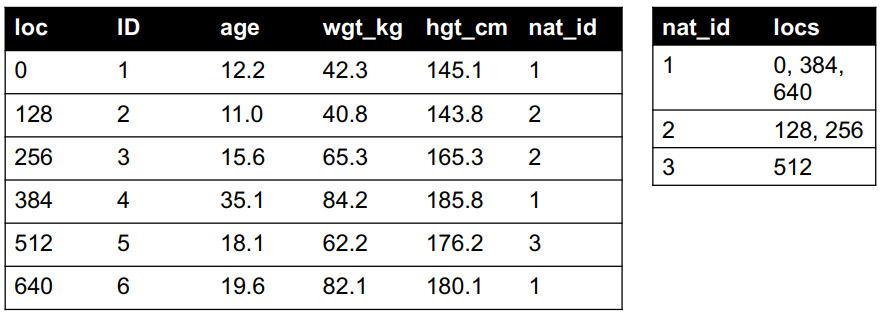
\includegraphics[width=372.75pt,height=150.4pt]{img/table_2.png}};
%Straight Lines [id:da26185218947017463] 
\draw [color={rgb, 255:red, 208; green, 2; blue, 27 }  ,draw opacity=1 ]   (107,45) -- (159.26,74.52) ;
\draw [shift={(161,75.5)}, rotate = 209.46] [color={rgb, 255:red, 208; green, 2; blue, 27 }  ,draw opacity=1 ][line width=0.75]    (10.93,-3.29) .. controls (6.95,-1.4) and (3.31,-0.3) .. (0,0) .. controls (3.31,0.3) and (6.95,1.4) .. (10.93,3.29)   ;
%Straight Lines [id:da2879956461468336] 
\draw [color={rgb, 255:red, 208; green, 2; blue, 27 }  ,draw opacity=1 ]   (107,45) -- (475.67,77.82) ;
\draw [shift={(477.67,78)}, rotate = 185.09] [color={rgb, 255:red, 208; green, 2; blue, 27 }  ,draw opacity=1 ][line width=0.75]    (10.93,-3.29) .. controls (6.95,-1.4) and (3.31,-0.3) .. (0,0) .. controls (3.31,0.3) and (6.95,1.4) .. (10.93,3.29)   ;
%Straight Lines [id:da19357327119760281] 
\draw [color={rgb, 255:red, 74; green, 144; blue, 226 }  ,draw opacity=1 ]   (413.67,32.67) -- (406.66,74.69) ;
\draw [shift={(406.33,76.67)}, rotate = 279.46] [color={rgb, 255:red, 74; green, 144; blue, 226 }  ,draw opacity=1 ][line width=0.75]    (10.93,-3.29) .. controls (6.95,-1.4) and (3.31,-0.3) .. (0,0) .. controls (3.31,0.3) and (6.95,1.4) .. (10.93,3.29)   ;
%Shape: Ellipse [id:dp8641831687478103] 
\draw  [color={rgb, 255:red, 74; green, 144; blue, 226 }  ,draw opacity=1 ][line width=3.75]  (375,186) .. controls (375,139.61) and (386.42,102) .. (400.5,102) .. controls (414.58,102) and (426,139.61) .. (426,186) .. controls (426,232.39) and (414.58,270) .. (400.5,270) .. controls (386.42,270) and (375,232.39) .. (375,186) -- cycle ;
%Shape: Ellipse [id:dp28836148924857286] 
\draw  [color={rgb, 255:red, 208; green, 2; blue, 27 }  ,draw opacity=1 ][line width=3.75]  (456.33,154.67) .. controls (456.33,125.21) and (464.69,101.33) .. (475,101.33) .. controls (485.31,101.33) and (493.67,125.21) .. (493.67,154.67) .. controls (493.67,184.12) and (485.31,208) .. (475,208) .. controls (464.69,208) and (456.33,184.12) .. (456.33,154.67) -- cycle ;
%Shape: Ellipse [id:dp4025421876242352] 
\draw  [color={rgb, 255:red, 208; green, 2; blue, 27 }  ,draw opacity=1 ][line width=3.75]  (142.33,186.67) .. controls (142.33,140.27) and (153.75,102.67) .. (167.83,102.67) .. controls (181.92,102.67) and (193.33,140.27) .. (193.33,186.67) .. controls (193.33,233.06) and (181.92,270.67) .. (167.83,270.67) .. controls (153.75,270.67) and (142.33,233.06) .. (142.33,186.67) -- cycle ;

% Text Node
\draw (58,20) node [anchor=north west][inner sep=0.75pt]   [align=left] {\textcolor[rgb]{0.82,0.01,0.11}{Primary Keys}};
% Text Node
\draw (368,8.67) node [anchor=north west][inner sep=0.75pt]   [align=left] {\textcolor[rgb]{0.29,0.56,0.89}{Foreign Keys}};


\end{tikzpicture}



}

There are four main types of relationships between keys. Here they are with some examples.

\begin{itemize}
	\item \textbf{One-to-many / Many-to-one}: A person can have one nationality, but a nationality can have many people associated with it.
	\item \textbf{One-to-one}: People each have one unique SSN- no conflicts.
	\item \textbf{One-to-one-or-none}: People can either have 1 car, or no car.
	\item \textbf{Many-to-many}: Cats and colors. Red can be on many cats, and many colors can be on a single cat.
\end{itemize}

Even though this system can sort of be replicated in \texttt{PANDAS}, \texttt{PANDAS} is not strictly a relational data system. Notably, it doesn't have notions of primary or foreign keys built in.

\begin{myproof}
Do heavy, rough lifting at the \textbf{relational database} level, (e.g. when you're deciding what sort of \texttt{SQL} queries to make) and then do the fine-grained slicing and dicing and visualization with \texttt{\textbf{PANDAS}}.
\end{myproof}

\subsection{SQL and SQLite}

\begin{tcolorbox}[title=Definition:,colframe=red!75!black,colback=red!5!white,arc=0pt,fonttitle=\bfseries]
\textbf{SQL} $\rightarrow$ Stands for 'Structured Query Language', and is the ANSI-standardized way for us to communicate with relational databases. Standard SQL commands like "Select", "Insert", "Update", "Delete", "Create", and "Drop" can be used to accomplish almost everything that one needs to do with a database.
\end{tcolorbox}

\hfill \break We use \textbf{SQLite}, an on-disk relational database management system, in order to interact with our databases. Most \textbf{RDMS}s connect to a server, which provides support for better concurrency, that sort of stuff takes longer to setup.\\

On the other hand, \texttt{SQLite} is pretty simple to install via \texttt{conda}, so we're going to go ahead and use it.\\

\texttt{SQLite} provides us with two main ways to communicate with the \texttt{SQL} database that it maintains. First of all, it gives us a cool GUI-based environment where we can deal with manipulating data manually, but it also allows us to write \texttt{SQL} statements to interact with it, whether that be from the command line or from within Python.\\

Here's an example of how a relational database fits into our workflow.\\\\

{

\centering



\tikzset{every picture/.style={line width=0.75pt}} %set default line width to 0.75pt        

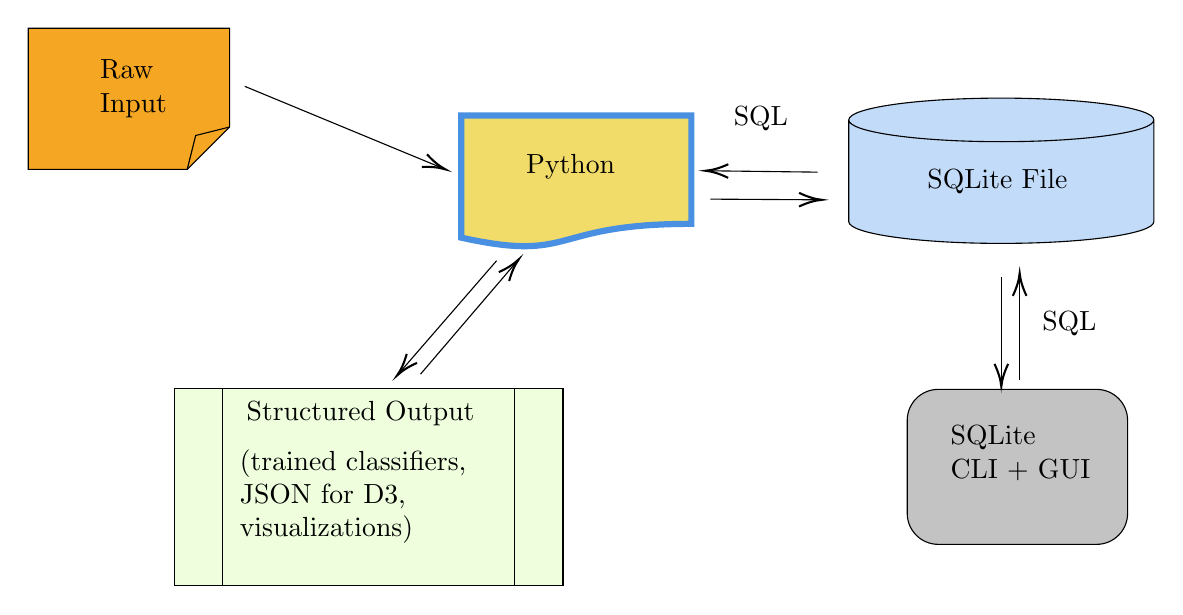
\begin{tikzpicture}[x=0.75pt,y=0.75pt,yscale=-1,xscale=1]
%uncomment if require: \path (0,300); %set diagram left start at 0, and has height of 300

%Shape: Folded Corner [id:dp17966687822939686] 
\draw  [fill={rgb, 255:red, 245; green, 166; blue, 35 }  ,fill opacity=1 ] (138.6,85.33) -- (62,85.33) -- (62,17.33) -- (159,17.33) -- (159,64.93) -- cycle -- (138.6,85.33) ; \draw   (159,64.93) -- (142.68,69.01) -- (138.6,85.33) ;
%Straight Lines [id:da19188911599755476] 
\draw    (166.33,45.33) -- (261.15,84.57) ;
\draw [shift={(263,85.33)}, rotate = 202.48] [color={rgb, 255:red, 0; green, 0; blue, 0 }  ][line width=0.75]    (10.93,-3.29) .. controls (6.95,-1.4) and (3.31,-0.3) .. (0,0) .. controls (3.31,0.3) and (6.95,1.4) .. (10.93,3.29)   ;
%Flowchart: Document [id:dp5212307516849849] 
\draw  [color={rgb, 255:red, 74; green, 144; blue, 226 }  ,draw opacity=1 ][fill={rgb, 255:red, 242; green, 220; blue, 105 }  ,fill opacity=1 ][line width=2.25]  (270.67,59.33) -- (381.5,59.33) -- (381.5,111.58) .. controls (312.23,111.58) and (326.08,130.42) .. (270.67,118.23) -- cycle ;
%Straight Lines [id:da2960662304041648] 
\draw    (390.67,99.67) -- (442.33,99.99) ;
\draw [shift={(444.33,100)}, rotate = 180.36] [color={rgb, 255:red, 0; green, 0; blue, 0 }  ][line width=0.75]    (10.93,-3.29) .. controls (6.95,-1.4) and (3.31,-0.3) .. (0,0) .. controls (3.31,0.3) and (6.95,1.4) .. (10.93,3.29)   ;
%Straight Lines [id:da4888130737896952] 
\draw    (442.33,86.67) -- (390.33,86.02) ;
\draw [shift={(388.33,86)}, rotate = 360.71000000000004] [color={rgb, 255:red, 0; green, 0; blue, 0 }  ][line width=0.75]    (10.93,-3.29) .. controls (6.95,-1.4) and (3.31,-0.3) .. (0,0) .. controls (3.31,0.3) and (6.95,1.4) .. (10.93,3.29)   ;
%Shape: Can [id:dp9185662032628965] 
\draw  [fill={rgb, 255:red, 194; green, 219; blue, 249 }  ,fill opacity=1 ] (604.33,61.5) -- (604.33,110.5) .. controls (604.33,116.3) and (571.43,121) .. (530.83,121) .. controls (490.24,121) and (457.33,116.3) .. (457.33,110.5) -- (457.33,61.5) .. controls (457.33,55.7) and (490.24,51) .. (530.83,51) .. controls (571.43,51) and (604.33,55.7) .. (604.33,61.5) .. controls (604.33,67.3) and (571.43,72) .. (530.83,72) .. controls (490.24,72) and (457.33,67.3) .. (457.33,61.5) ;
%Straight Lines [id:da4630895722743661] 
\draw    (530.83,137.33) -- (530.83,188) ;
\draw [shift={(530.83,190)}, rotate = 270] [color={rgb, 255:red, 0; green, 0; blue, 0 }  ][line width=0.75]    (10.93,-3.29) .. controls (6.95,-1.4) and (3.31,-0.3) .. (0,0) .. controls (3.31,0.3) and (6.95,1.4) .. (10.93,3.29)   ;
%Straight Lines [id:da7457072915555859] 
\draw    (539.67,186.67) -- (539.67,137.33) ;
\draw [shift={(539.67,135.33)}, rotate = 450] [color={rgb, 255:red, 0; green, 0; blue, 0 }  ][line width=0.75]    (10.93,-3.29) .. controls (6.95,-1.4) and (3.31,-0.3) .. (0,0) .. controls (3.31,0.3) and (6.95,1.4) .. (10.93,3.29)   ;
%Flowchart: Prodefined Process [id:dp6652571645774823] 
\draw  [fill={rgb, 255:red, 239; green, 255; blue, 221 }  ,fill opacity=1 ] (132.33,191) -- (319.67,191) -- (319.67,286) -- (132.33,286) -- cycle ; \draw   (155.75,191) -- (155.75,286) ; \draw   (296.25,191) -- (296.25,286) ;
%Straight Lines [id:da7038486863895331] 
\draw    (287.67,129.33) -- (240.98,183.16) ;
\draw [shift={(239.67,184.67)}, rotate = 310.94] [color={rgb, 255:red, 0; green, 0; blue, 0 }  ][line width=0.75]    (10.93,-3.29) .. controls (6.95,-1.4) and (3.31,-0.3) .. (0,0) .. controls (3.31,0.3) and (6.95,1.4) .. (10.93,3.29)   ;
%Rounded Rect [id:dp7535419443712124] 
\draw  [fill={rgb, 255:red, 155; green, 155; blue, 155 }  ,fill opacity=0.6 ] (485.5,206.27) .. controls (485.5,198.02) and (492.19,191.33) .. (500.43,191.33) -- (576.73,191.33) .. controls (584.98,191.33) and (591.67,198.02) .. (591.67,206.27) -- (591.67,251.07) .. controls (591.67,259.31) and (584.98,266) .. (576.73,266) -- (500.43,266) .. controls (492.19,266) and (485.5,259.31) .. (485.5,251.07) -- cycle ;
%Straight Lines [id:da07613681473682243] 
\draw    (251,184) -- (297.03,130.19) ;
\draw [shift={(298.33,128.67)}, rotate = 490.54] [color={rgb, 255:red, 0; green, 0; blue, 0 }  ][line width=0.75]    (10.93,-3.29) .. controls (6.95,-1.4) and (3.31,-0.3) .. (0,0) .. controls (3.31,0.3) and (6.95,1.4) .. (10.93,3.29)   ;

% Text Node
\draw (95.33,31.33) node [anchor=north west][inner sep=0.75pt]   [align=left] {Raw\\Input};
% Text Node
\draw (300.67,77) node [anchor=north west][inner sep=0.75pt]   [align=left] {Python};
% Text Node
\draw (494,84) node [anchor=north west][inner sep=0.75pt]   [align=left] {SQLite File};
% Text Node
\draw (400.67,53.67) node [anchor=north west][inner sep=0.75pt]   [align=left] {SQL};
% Text Node
\draw (549.33,152.67) node [anchor=north west][inner sep=0.75pt]   [align=left] {SQL};
% Text Node
\draw (505.17,207.67) node [anchor=north west][inner sep=0.75pt]   [align=left] {SQLite\\CLI + GUI};
% Text Node
\draw (166,196) node [anchor=north west][inner sep=0.75pt]   [align=left] {Structured Output};
% Text Node
\draw (162.67,219) node [anchor=north west][inner sep=0.75pt]   [align=left] {(trained classifiers,\\JSON for D3,\\visualizations)};


\end{tikzpicture}


}

To work with \texttt{SQLite} in Python3, simply install and import the \texttt{SQLite3} package, and use that.

\subsection{Joining Data}

A \textbf{join} operations merges two or more tables into a single relation, based on their columns. There are four total types of join operations.\\ 

\begin{myproof}
Formally, the way we format join statements is the following:\\\\
\texttt{<type of join> join (<left table>, <right table>) on (<left table column>, <right table column>)}\\

Example: \texttt{Right join (cats, visits) on (id, cat\_id)}
\end{myproof}

\subsubsection{Types of Joins}

\begin{itemize}
	\item \textbf{Inner Join} $\rightarrow$ Returns merged rows that share the \textbf{same} value in the column that they are being joined on. Let's say we had the following two tables and wanted to join them.\\
	
	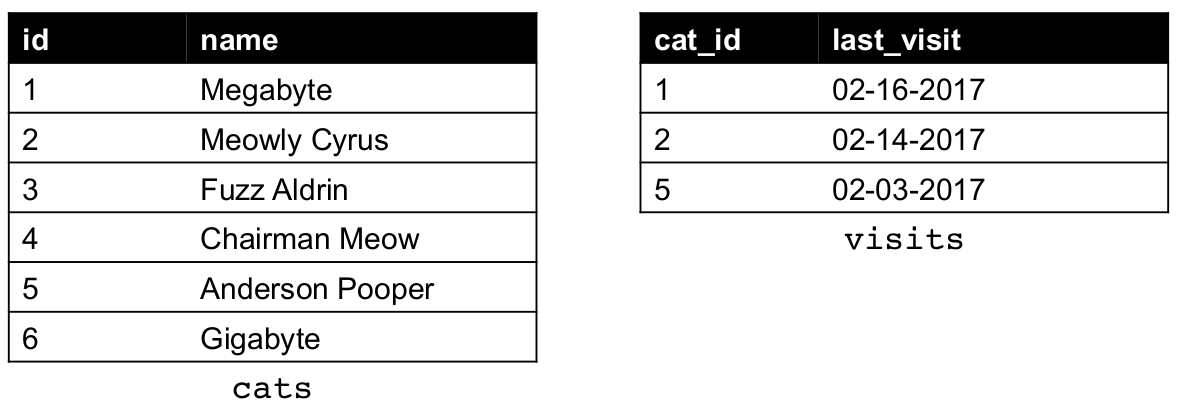
\includegraphics[scale=0.35]{img/table_3.png}\\
	
	In order to perform an inner join on these two tables, we need to pick a column to 'join them on'. Here, let's inner join these two tables on \texttt{id} and \texttt{cat\_id}. The result would look like this:\\
	
	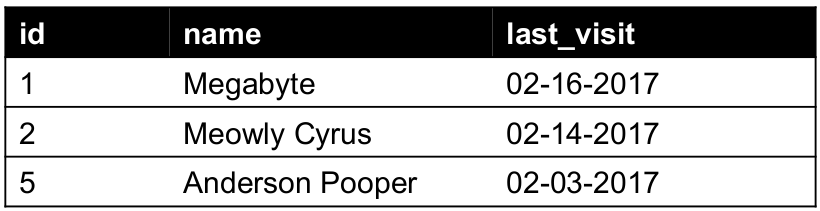
\includegraphics[scale=0.35]{img/table_4.png}\\
	
	Inner joins are the most common type of joins; they get us the results that are shared by both tables.
	
	\item \textbf{Left Join} $\rightarrow$ A left join gets us \textbf{all} the results from the \textbf{left} table, but only \textbf{some} (the corresponding matching results) from the \textbf{right table}. So, what happens if we Left Joined \texttt{cats} and \texttt{visits} on \texttt{(id, cat\_id)}?\\
	
	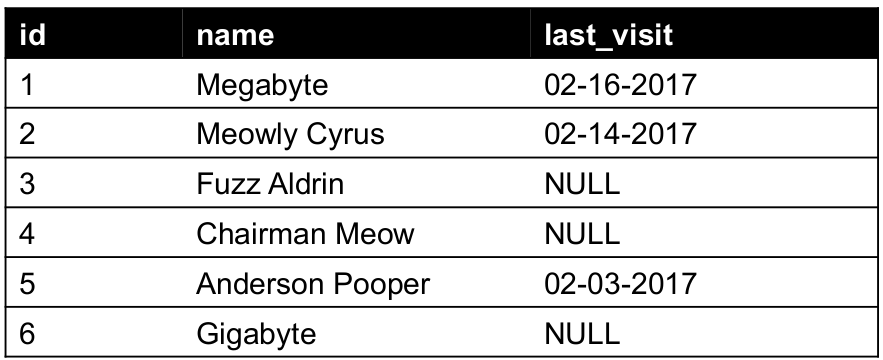
\includegraphics[scale=0.35]{img/table_5.png}\\
	
	You'll notice that the fields that we couldn't fill out get populated with \textbf{\texttt{NULL}}.
	
	\item \textbf{Right Join} $\rightarrow$ A right join gets us \textbf{all} the results from the \textbf{right} table, but only \textbf{some} (the corresponding matching results) from the \textbf{left} table. Here's an example, with updated \texttt{cats} and \texttt{visits} tables.\\
	
	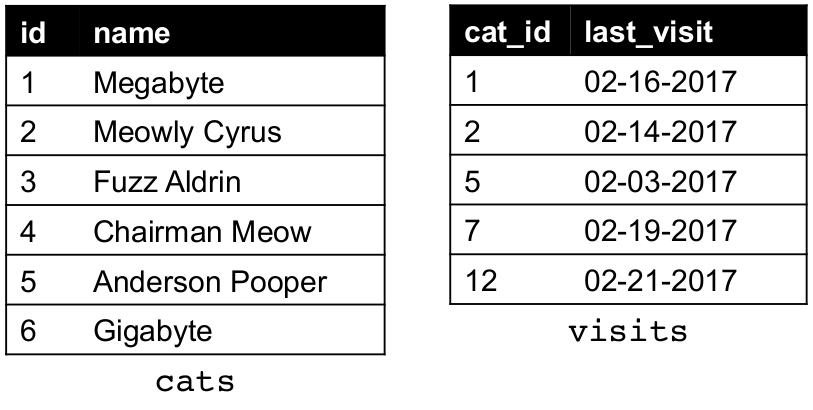
\includegraphics[scale=0.35]{img/table_6.png}\\
	
	If we were to perform a right join on these two tables, here's what would happen. It's basically just a flipped version of the left join.\\
	
	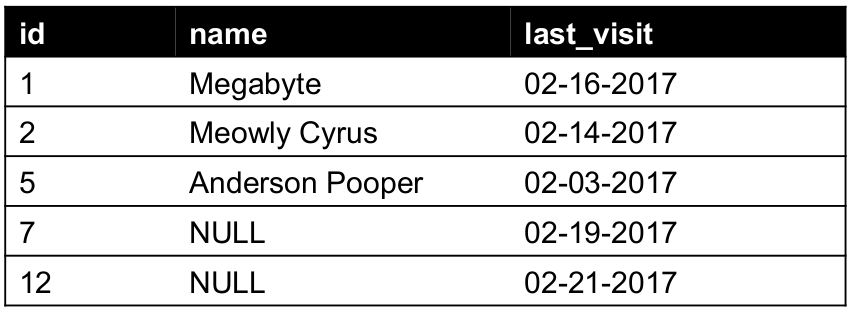
\includegraphics[scale=0.35]{img/table_7.png}\\
	
	Again, this time, notice how the row entries missing from the left table are now set to \texttt{\textbf{NULL}}
	
	\item \textbf{Full Outer Join} $\rightarrow$ The full outer join combines the left and right join. It's analogous to a \textbf{union} operation. Here's an example of a full outer join of \texttt{cats} and \texttt{visits} on \texttt{id} and \texttt{cat\_id}.\\
	
	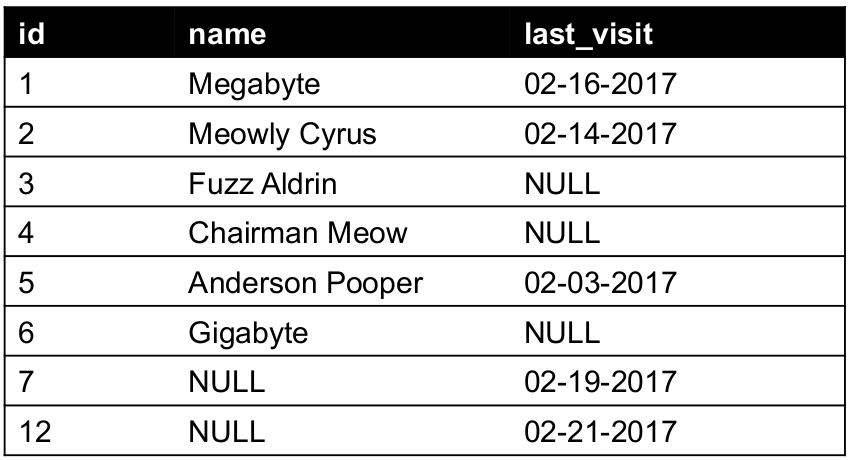
\includegraphics[scale=0.35]{img/table_8.png}\\
	
\end{itemize}

\subsubsection{Syntax in PANDAS}

Here's how to write some basic join syntax in \texttt{PANDAS}. This should be easy once you learn how to phrase join statements- you're basically just translating it into code.\\

First, this is how you'd read from \texttt{SQLite} (or any other database you're hooked up to) using \texttt{Pandas} and generate the appropriate dataframes to work with.\\

{\centering
\begin{lstlisting}[language=python]
# establish dataframes from SQL
df_cats = pd.read_sql_query("SELECT * from cats", conn)
df_visits = pd.read_sql_query("SELECT * from visits", conn)
\end{lstlisting}
}

\hfill \break Now, here's how to do the joins.

{\centering
\begin{lstlisting}[language=python]
# inner join
df_cats.merge(df_visits, how = "inner",
              left_on = "id", right_on = "cat_id")
              
# left join
df_cats.merge(df_visits, how = "left",
              left_on = "id", right_on = "cat_id")
              
# right join
df_cats.merge(df_visits, how = "right",
              left_on = "id", right_on = "cat_id")
              
# full outer join
df_cats.merge(df_visits, how = "outer",
              left_on = "id", right_on = "cat_id")
\end{lstlisting}
}

There are also ways you can perform most of these joins via SQL (save for the right join), but I would prefer doing them from Python. As such, I won't include the \texttt{SQL} syntax here.

\hfill \break
\begin{tcolorbox}[title=Aside: Raw \texttt{SQL} with Pandas,colframe=black,colback=white,arc=0pt,fonttitle=\bfseries]
If you want to use raw \texttt{SQL} queries to interact with \texttt{PANDAS} dataframes, you are free to do so when you use the \texttt{PandaSQL} library.
\end{tcolorbox}

\subsubsection{Visual Example}

Here's a neat way to visualize joins using Venn Diagrams.\\\\

{
\centering



\tikzset{every picture/.style={line width=0.75pt}} %set default line width to 0.75pt        

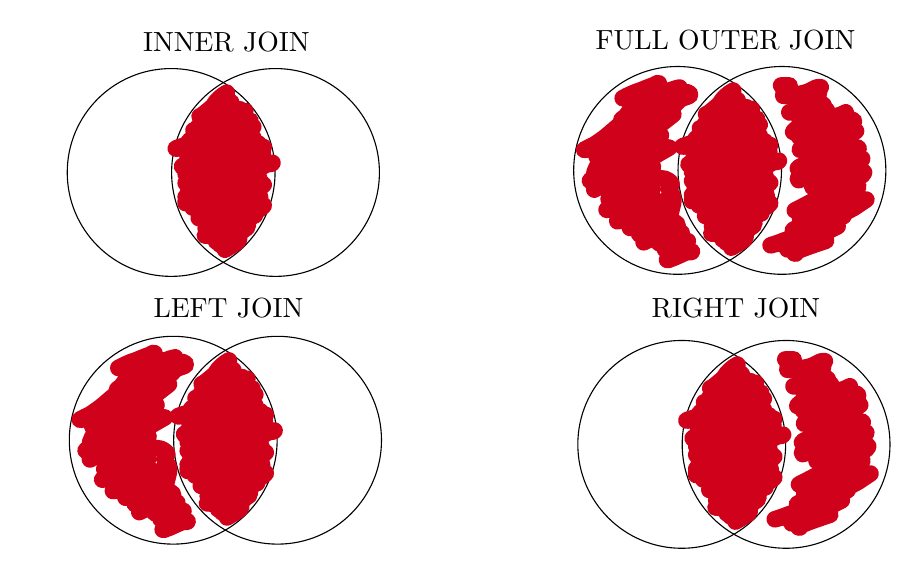
\begin{tikzpicture}[x=0.75pt,y=0.75pt,yscale=-1,xscale=1]
%uncomment if require: \path (0,300); %set diagram left start at 0, and has height of 300

%Shape: Circle [id:dp6533662955757997] 
\draw   (116,75.43) .. controls (116,47.78) and (138.42,25.37) .. (166.07,25.37) .. controls (193.72,25.37) and (216.13,47.78) .. (216.13,75.43) .. controls (216.13,103.08) and (193.72,125.5) .. (166.07,125.5) .. controls (138.42,125.5) and (116,103.08) .. (116,75.43) -- cycle ;
%Shape: Circle [id:dp3081615610888653] 
\draw   (166.28,75.43) .. controls (166.28,47.78) and (188.69,25.37) .. (216.35,25.37) .. controls (244,25.37) and (266.41,47.78) .. (266.41,75.43) .. controls (266.41,103.08) and (244,125.5) .. (216.35,125.5) .. controls (188.69,125.5) and (166.28,103.08) .. (166.28,75.43) -- cycle ;
%Shape: Free Drawing [id:dp702537410998645] 
\draw  [color={rgb, 255:red, 208; green, 2; blue, 27 }  ,draw opacity=1 ][line width=6] [line join = round][line cap = round] (192.9,36.98) .. controls (190.46,38.37) and (188.04,40.43) .. (186.56,42.9) .. controls (186.33,43.28) and (187.42,42.66) .. (187.83,42.48) .. controls (188.93,41.99) and (190.11,41.71) .. (191.21,41.21) .. controls (191.67,41) and (192.02,40.59) .. (192.47,40.36) .. controls (192.76,40.22) and (193.63,39.89) .. (193.32,39.94) .. controls (189.56,40.57) and (187.18,42.64) .. (184.45,45.01) .. controls (183.08,46.19) and (181.68,47.33) .. (180.22,48.39) .. controls (180.11,48.47) and (179.67,48.45) .. (179.8,48.39) .. controls (184.42,46.23) and (189.08,44.13) .. (193.74,42.05) .. controls (194.15,41.87) and (195.45,41.63) .. (195.01,41.63) .. controls (191.07,41.63) and (185.3,47.08) .. (183.18,48.81) .. controls (182.25,49.57) and (181.44,50.46) .. (180.64,51.35) .. controls (180.17,51.87) and (178.75,52.72) .. (179.38,53.04) .. controls (180.29,53.5) and (181.39,52.59) .. (182.33,52.19) .. controls (187.87,49.91) and (193.3,47.36) .. (198.81,45.01) .. controls (198.94,44.96) and (199.37,44.98) .. (199.23,45.01) .. controls (193.44,46.46) and (190.25,48.45) .. (184.45,51.35) .. controls (183.49,51.83) and (182.44,52.12) .. (181.49,52.62) .. controls (180.04,53.39) and (178.71,54.37) .. (177.26,55.15) .. controls (177.14,55.22) and (176.71,55.2) .. (176.84,55.15) .. controls (184.24,52.69) and (191.53,49.91) .. (198.81,47.12) .. controls (199.64,46.81) and (200.58,46.74) .. (201.35,46.28) .. controls (201.52,46.18) and (201.96,45.8) .. (201.77,45.86) .. controls (194.66,48.05) and (187.64,50.93) .. (181.49,55.15) .. controls (179.84,56.29) and (178.35,57.64) .. (176.84,58.95) .. controls (176.16,59.55) and (174.09,60.01) .. (174.73,60.64) .. controls (175.89,61.81) and (179.51,59.7) .. (180.64,59.38) .. controls (187.06,57.54) and (193.05,55.09) .. (199.23,52.62) .. controls (199.81,52.39) and (204.3,51.45) .. (204.3,50.5) .. controls (204.3,49.85) and (200.11,51.76) .. (200.08,51.77) .. controls (198.42,52.29) and (196.69,52.57) .. (195.01,53.04) .. controls (193.16,53.56) and (191.32,54.09) .. (189.52,54.73) .. controls (186.03,55.96) and (182.54,57.21) .. (178.95,58.11) .. controls (178.76,58.16) and (179.19,57.77) .. (179.38,57.69) .. controls (181.18,56.91) and (183.08,56.38) .. (184.87,55.57) .. controls (187.45,54.41) and (189.86,52.86) .. (192.47,51.77) .. controls (194,51.14) and (195.96,51.25) .. (197.12,50.08) .. controls (197.75,49.45) and (198.86,49.64) .. (199.66,49.24) .. controls (199.83,49.15) and (200.27,48.78) .. (200.08,48.81) .. controls (198.41,49.15) and (196.95,50.17) .. (195.43,50.93) .. controls (188.39,54.45) and (180.52,56.66) .. (174.31,61.49) .. controls (173.86,61.84) and (175.44,61.57) .. (176,61.49) .. controls (178.4,61.15) and (180.83,60.86) .. (183.18,60.22) .. controls (190.7,58.18) and (198.12,55.74) .. (205.57,53.46) .. controls (206.13,53.29) and (204.42,53.66) .. (203.88,53.88) .. controls (203.01,54.26) and (202.19,54.73) .. (201.35,55.15) .. controls (198.64,56.5) and (195.95,57.89) .. (193.32,59.38) .. controls (187.76,62.5) and (181.69,67.1) .. (176,69.94) .. controls (175.74,70.07) and (176.58,70.05) .. (176.84,69.94) .. controls (182.66,67.5) and (188.41,64.92) .. (194.16,62.33) .. controls (195.31,61.82) and (196.44,61.26) .. (197.54,60.64) .. controls (198.09,60.34) and (199.85,59.68) .. (199.23,59.8) .. controls (193.97,60.81) and (188.71,61.98) .. (183.6,63.6) .. controls (181.94,64.13) and (180.21,64.39) .. (178.53,64.87) .. controls (178.23,64.96) and (177.42,65.47) .. (177.69,65.29) .. controls (183.06,61.71) and (191.12,59.19) .. (197.12,57.69) .. controls (197.82,57.51) and (203.24,56.18) .. (203.46,56.84) .. controls (203.76,57.74) and (201.7,57.57) .. (200.92,58.11) .. controls (199.86,58.85) and (199.09,59.99) .. (197.97,60.64) .. controls (191.6,64.37) and (185.04,67.75) .. (178.53,71.21) .. controls (178.14,71.42) and (176.82,71.63) .. (177.26,71.63) .. controls (178.78,71.63) and (180.08,70.5) .. (181.49,69.94) .. controls (188.6,67.09) and (196.2,65.64) .. (203.46,63.18) .. controls (204.9,62.69) and (209.04,60.81) .. (207.68,61.49) .. controls (198.98,65.84) and (191.74,68.69) .. (183.18,73.74) .. controls (181.98,74.45) and (180.49,74.6) .. (179.38,75.43) .. controls (178.8,75.86) and (180.8,75.2) .. (181.49,75.01) .. controls (183.31,74.51) and (184.84,73.25) .. (186.56,72.48) .. controls (190.54,70.68) and (194.71,69.34) .. (198.81,67.83) .. controls (200.95,67.04) and (203.06,66.2) .. (205.15,65.29) .. controls (205.33,65.21) and (205.75,64.79) .. (205.57,64.87) .. controls (200.2,67.29) and (194.7,70.07) .. (189.52,72.9) .. controls (187.63,73.93) and (185.88,75.19) .. (184.02,76.28) .. controls (183.42,76.63) and (181.63,77.55) .. (182.33,77.55) .. controls (186.09,77.55) and (202.6,70.12) .. (203.04,69.94) .. controls (204.62,69.31) and (206.08,68.4) .. (207.68,67.83) .. controls (208.08,67.69) and (209.37,67.83) .. (208.95,67.83) .. controls (207.75,67.83) and (206.65,68.56) .. (205.57,69.1) .. controls (199.71,72.02) and (193.71,74.67) .. (187.83,77.55) .. controls (185.67,78.6) and (178.98,81.36) .. (179.8,81.77) .. controls (180.96,82.35) and (182.37,81.34) .. (183.6,80.93) .. controls (186.86,79.84) and (190.1,78.73) .. (193.32,77.55) .. controls (197.88,75.87) and (202.61,74.72) .. (207.26,73.32) .. controls (209.75,72.57) and (212.19,70.79) .. (214.87,70.79) .. controls (215.07,70.79) and (214.64,71.15) .. (214.44,71.21) .. controls (213.62,71.44) and (212.7,71.3) .. (211.91,71.63) .. controls (210.28,72.3) and (208.88,73.47) .. (207.26,74.17) .. controls (200.92,76.9) and (194.36,79.1) .. (187.83,81.35) .. controls (185.5,82.15) and (181.07,84.31) .. (181.07,84.31) .. controls (181.07,84.31) and (182.17,83.43) .. (182.76,83.04) .. controls (185.73,81.05) and (188.73,79.56) .. (192.05,77.97) .. controls (193.87,77.1) and (198.97,76.86) .. (197.54,75.43) .. controls (196.23,74.12) and (193.83,75.77) .. (192.05,76.28) .. controls (187.93,77.45) and (181.35,80.5) .. (176.84,80.5) .. controls (176.7,80.5) and (177.14,80.57) .. (177.26,80.5) .. controls (179.13,79.44) and (180.89,78.19) .. (182.76,77.12) .. controls (183.85,76.5) and (185.03,76.04) .. (186.14,75.43) .. controls (188.13,74.35) and (190.05,73.12) .. (192.05,72.05) .. controls (192.18,71.99) and (192.62,72.05) .. (192.47,72.05) .. controls (186.99,72.05) and (181.92,74.16) .. (176.84,75.43) .. controls (176.39,75.54) and (173.04,76.28) .. (173.04,76.28) .. controls (173.04,76.28) and (176.8,75.08) .. (178.53,74.17) .. controls (181.59,72.54) and (184.69,70.98) .. (187.83,69.52) .. controls (188.23,69.33) and (187,69.88) .. (186.56,69.94) .. controls (185.72,70.04) and (184.86,69.86) .. (184.02,69.94) .. controls (180.95,70.25) and (176.33,71.07) .. (173.88,71.63) .. controls (173.02,71.83) and (170.62,72.98) .. (171.35,72.48) .. controls (174.68,70.16) and (178.53,68.49) .. (181.49,65.71) .. controls (181.82,65.4) and (176.65,66.76) .. (176,66.98) .. controls (175.32,67.21) and (173.17,67.35) .. (173.88,67.4) .. controls (176.27,67.6) and (178.68,67.28) .. (181.07,67.4) .. controls (181.38,67.42) and (181.95,67.51) .. (181.91,67.83) .. controls (181.84,68.5) and (179.98,72.96) .. (179.38,73.74) .. controls (177.55,76.11) and (175.51,78.32) .. (173.46,80.5) .. controls (173.36,80.61) and (172.9,80.5) .. (173.04,80.5) .. controls (176.8,80.5) and (180.01,78.57) .. (183.6,77.97) .. controls (183.74,77.94) and (183.3,77.89) .. (183.18,77.97) .. controls (181.59,79.03) and (180.13,80.29) .. (178.53,81.35) .. controls (177.16,82.26) and (175.62,82.9) .. (174.31,83.88) .. controls (174.08,84.05) and (174.88,83.94) .. (175.15,83.88) .. controls (176.15,83.66) and (177.16,83.42) .. (178.11,83.04) .. controls (179.98,82.29) and (181.72,81.23) .. (183.6,80.5) .. controls (184.08,80.32) and (182.74,81.04) .. (182.33,81.35) .. controls (179.85,83.21) and (177.6,85.36) .. (175.15,87.26) .. controls (175.04,87.35) and (174.59,87.3) .. (174.73,87.26) .. controls (181.95,85.46) and (188.64,82.47) .. (195.85,80.5) .. controls (197.03,80.18) and (191.9,82.87) .. (185.29,86.84) .. controls (182.79,88.34) and (178.78,90.37) .. (176.42,92.33) .. controls (176.31,92.42) and (176.71,92.38) .. (176.84,92.33) .. controls (183.9,89.56) and (190.98,86.83) .. (197.97,83.88) .. controls (198.63,83.6) and (196.51,84.02) .. (195.85,84.31) .. controls (193.26,85.44) and (190.81,86.89) .. (188.25,88.11) .. controls (187.56,88.44) and (186.81,88.61) .. (186.14,88.95) .. controls (185.96,89.04) and (185.54,89.46) .. (185.71,89.38) .. controls (191.02,86.72) and (195.95,83.01) .. (201.35,80.5) .. controls (203.41,79.54) and (206.67,80) .. (207.68,77.97) .. controls (208.01,77.33) and (206.22,78.09) .. (205.57,78.39) .. controls (203.46,79.37) and (201.27,80.22) .. (199.23,81.35) .. controls (198.52,81.75) and (196.39,82.98) .. (197.12,82.62) .. controls (198.65,81.85) and (206.83,76.7) .. (208.11,77.12) .. controls (209.07,77.44) and (206.45,78.3) .. (205.57,78.81) .. controls (204.76,79.29) and (203.83,79.57) .. (203.04,80.08) .. controls (199.91,82.07) and (196.97,83.98) .. (193.74,86) .. controls (193.1,86.4) and (190.91,87.07) .. (191.63,86.84) .. controls (194.01,86.1) and (196.4,85.36) .. (198.81,84.73) .. controls (209.07,82.05) and (192.6,87.75) .. (189.52,90.22) .. controls (188.92,90.69) and (190.9,89.59) .. (191.63,89.38) .. controls (192.45,89.13) and (193.36,89.26) .. (194.16,88.95) .. controls (196.34,88.12) and (198.36,86.91) .. (200.5,86) .. controls (201.57,85.54) and (203.88,85.15) .. (203.88,85.15) .. controls (203.88,85.15) and (203.29,85.02) .. (203.04,85.15) .. controls (198.52,87.41) and (194.22,90.08) .. (189.94,92.76) .. controls (188.91,93.4) and (185.82,95.2) .. (186.98,94.87) .. controls (191.19,93.67) and (203.36,88.5) .. (205.15,87.69) .. controls (205.72,87.43) and (207.44,86.64) .. (206.84,86.84) .. controls (200.15,89.07) and (194.05,92.81) .. (187.83,96.14) .. controls (187.27,96.43) and (185.53,97.13) .. (186.14,96.98) .. controls (190.69,95.84) and (199.62,90.64) .. (203.04,90.64) .. controls (203.62,90.64) and (201.86,90.79) .. (201.35,91.07) .. controls (196.67,93.6) and (192.38,96.78) .. (187.83,99.52) .. controls (187.12,99.94) and (184.98,100.42) .. (185.71,100.78) .. controls (186.33,101.09) and (188.71,99.66) .. (189.09,99.52) .. controls (192.17,98.33) and (195.32,97.33) .. (198.39,96.14) .. controls (200.39,95.36) and (202.36,94.51) .. (204.3,93.6) .. controls (204.48,93.52) and (204.93,93.18) .. (204.73,93.18) .. controls (200.95,93.18) and (197.28,97.33) .. (194.59,99.09) .. controls (192.32,100.58) and (189.71,101.48) .. (187.4,102.9) .. controls (186.49,103.46) and (189.35,101.99) .. (190.36,101.63) .. controls (193,100.67) and (195.8,100.17) .. (198.39,99.09) .. controls (199.22,98.75) and (199.68,97.76) .. (200.5,97.4) .. controls (202.01,96.74) and (206.73,95.26) .. (205.15,95.71) .. controls (201.62,96.72) and (189.19,103.4) .. (187.4,105.01) .. controls (186.44,105.88) and (189.98,104.59) .. (191.21,104.16) .. controls (195.97,102.52) and (196.97,101.54) .. (200.5,100.36) .. controls (200.64,100.32) and (200.21,100.3) .. (200.08,100.36) .. controls (198.78,101.01) and (197.48,101.66) .. (196.28,102.47) .. controls (193.95,104.06) and (191.69,105.75) .. (189.52,107.54) .. controls (188.97,107.99) and (187.16,109.03) .. (187.83,108.81) .. controls (192.71,107.18) and (198.47,105.16) .. (202.61,102.05) .. controls (203.22,101.6) and (201.12,102.46) .. (200.5,102.9) .. controls (199.6,103.53) and (198.89,104.41) .. (197.97,105.01) .. controls (197.3,105.44) and (189.52,109.5) .. (189.52,110.08) .. controls (189.52,111.24) and (191.77,109.5) .. (192.9,109.23) .. controls (194.92,108.76) and (197.24,109.11) .. (198.81,107.54) .. controls (199.03,107.32) and (198.21,107.77) .. (197.97,107.97) .. controls (197.5,108.34) and (197.16,108.85) .. (196.7,109.23) .. controls (195.3,110.4) and (193.63,111.82) .. (192.05,112.61) .. controls (191.32,112.98) and (193.45,111.75) .. (194.16,111.35) .. controls (195.32,110.69) and (196.46,110) .. (197.54,109.23) .. controls (200.01,107.51) and (196.39,108.58) .. (196.7,107.97) .. controls (197.84,105.68) and (202.71,101.76) .. (203.04,100.78) .. controls (203.4,99.68) and (197.78,101.56) .. (197.54,101.63) .. controls (197.24,101.71) and (196.7,102.37) .. (196.7,102.05) .. controls (196.7,100.79) and (198.99,100.99) .. (200.08,100.36) .. controls (201.3,99.66) and (202.29,98.61) .. (203.46,97.83) .. controls (204.26,97.29) and (205.19,96.67) .. (205.99,96.14) .. controls (206.11,96.06) and (206.56,96.14) .. (206.42,96.14) .. controls (205.37,96.14) and (203.56,96.2) .. (202.61,96.56) .. controls (200.73,97.27) and (198.98,98.3) .. (197.12,99.09) .. controls (196.99,99.15) and (196.57,99.16) .. (196.7,99.09) .. controls (201.07,96.91) and (207.21,94.92) .. (210.64,91.49) .. controls (211.24,90.89) and (208.93,91.31) .. (208.11,91.49) .. controls (206.23,91.88) and (204.43,92.57) .. (202.61,93.18) .. controls (201.74,93.47) and (201.38,93.31) .. (200.5,93.6) .. controls (200.31,93.66) and (199.94,94.16) .. (200.08,94.02) .. controls (202.65,91.45) and (206.22,90.08) .. (208.95,87.69) .. controls (209.91,86.85) and (206.32,87.6) .. (205.15,88.11) .. controls (203.53,88.82) and (202.1,89.9) .. (200.5,90.64) .. controls (199.98,90.89) and (199.36,90.88) .. (198.81,91.07) .. controls (198.51,91.17) and (197.72,91.69) .. (197.97,91.49) .. controls (202.08,88.06) and (203.07,88.14) .. (208.53,84.73) .. controls (208.91,84.49) and (207.69,85.04) .. (207.26,85.15) .. controls (205.97,85.47) and (204.65,85.82) .. (203.46,86.42) .. controls (203.28,86.51) and (202.9,86.98) .. (203.04,86.84) .. controls (203.89,85.98) and (204.98,85.38) .. (205.99,84.73) .. controls (207.44,83.8) and (208.88,82.84) .. (210.22,81.77) .. controls (210.38,81.65) and (210.84,81.35) .. (210.64,81.35) .. controls (208.75,81.35) and (206.42,82.74) .. (204.73,83.46) .. controls (203.51,83.98) and (200.24,86.31) .. (201.35,85.57) .. controls (203.96,83.83) and (206.76,81.82) .. (209.37,80.08) .. controls (209.49,80) and (209.08,80.02) .. (208.95,80.08) .. controls (206.11,81.43) and (203.26,82.78) .. (200.5,84.31) .. controls (194.96,87.37) and (190.26,91.21) .. (184.87,94.45) .. controls (183.39,95.33) and (180.11,95.94) .. (179.38,97.4) .. controls (179.31,97.53) and (179.67,97.45) .. (179.8,97.4) .. controls (180.77,97.08) and (181.86,96.21) .. (182.76,95.71) .. controls (185.19,94.37) and (188.2,93.66) .. (189.94,91.49) .. controls (190.73,90.5) and (187.39,91.28) .. (186.14,91.49) .. controls (183.81,91.88) and (179.38,91.24) .. (179.38,93.6) .. controls (179.38,93.62) and (187.94,89.2) .. (188.25,88.95) .. controls (188.6,88.67) and (187.33,89.1) .. (186.98,89.38) .. controls (185.89,90.25) and (185.05,91.38) .. (184.02,92.33) .. controls (183.07,93.22) and (180.15,93.95) .. (181.07,94.87) .. controls (182.37,96.17) and (186.37,94.02) .. (188.25,94.02) .. controls (190.25,94.02) and (185.74,97.14) .. (184.45,98.67) .. controls (184.06,99.13) and (182.6,100.08) .. (183.18,99.94) .. controls (184.44,99.62) and (185.73,99.43) .. (186.98,99.09) .. controls (187.29,99.01) and (187.83,98.36) .. (187.83,98.67) .. controls (187.83,100.08) and (185.68,100.52) .. (184.45,101.21) .. controls (183.83,101.55) and (182.07,102.61) .. (182.76,102.47) .. controls (184.2,102.18) and (185.6,101.71) .. (186.98,101.21) .. controls (187.17,101.14) and (187.54,100.64) .. (187.4,100.78) .. controls (185.95,102.24) and (183.28,103.95) .. (182.33,105.85) .. controls (182.07,106.37) and (183.47,105.61) .. (184.02,105.43) .. controls (184.07,105.41) and (187.4,104.31) .. (187.4,104.16) .. controls (187.4,103.06) and (183.86,106.72) .. (184.87,106.28) .. controls (186.26,105.66) and (187.66,105.07) .. (189.09,104.59) .. controls (189.52,104.44) and (188.67,105.41) .. (188.67,105.85) .. controls (188.67,105.99) and (188.58,105.54) .. (188.67,105.43) .. controls (189.45,104.52) and (190.47,103.84) .. (191.21,102.9) .. controls (194.81,98.26) and (194.45,97.77) .. (197.12,92.76) .. controls (198.13,90.86) and (200.6,89.15) .. (199.23,86.42) .. controls (198.66,85.28) and (194.96,87.18) .. (195.43,86) .. controls (196.49,83.35) and (199.24,81.54) .. (200.08,78.81) .. controls (200.29,78.14) and (198.58,78.47) .. (197.97,78.81) .. controls (195.95,79.93) and (194.26,81.58) .. (192.47,83.04) .. controls (192.23,83.24) and (193.06,82.79) .. (193.32,82.62) .. controls (194.89,81.52) and (198.49,81.08) .. (197.97,79.24) .. controls (197.46,77.47) and (194.3,79.43) .. (192.47,79.66) .. controls (189.92,79.98) and (187.43,81.1) .. (184.87,80.93) .. controls (184.45,80.9) and (184.74,80.06) .. (184.87,79.66) .. controls (185.48,77.84) and (187.68,77.81) .. (186.98,75.01) .. controls (186.81,74.33) and (185.54,74.8) .. (184.87,75.01) .. controls (181.18,76.16) and (180.2,77.55) .. (177.26,77.55) .. controls (176.76,77.55) and (178.13,77) .. (178.53,76.7) .. controls (179.34,76.09) and (180.16,75.46) .. (181.07,75.01) .. controls (181.07,75.01) and (195.18,70.02) .. (197.12,66.14) .. controls (197.82,64.75) and (194.01,65.93) .. (192.47,65.71) .. controls (191.66,65.6) and (193.88,64.86) .. (194.59,64.45) .. controls (197.09,62.98) and (199.44,61.14) .. (202.19,60.22) .. controls (202.31,60.18) and (206.08,59.04) .. (205.57,58.53) .. controls (205.42,58.39) and (204.8,58.89) .. (204.73,58.95) .. controls (203.4,60.01) and (201.52,60.75) .. (200.92,62.33) .. controls (200.63,63.13) and (202.62,62.4) .. (203.46,62.33) .. controls (204.59,62.25) and (205.73,62.16) .. (206.84,61.91) .. controls (207.27,61.82) and (208.31,61.09) .. (208.11,61.49) .. controls (207.39,62.92) and (205.61,63.54) .. (204.73,64.87) .. controls (204.31,65.5) and (206.09,64.15) .. (206.84,64.02) .. controls (208.02,63.83) and (208.64,63.89) .. (209.8,63.6) .. controls (210.1,63.53) and (210.88,62.97) .. (210.64,63.18) .. controls (208.82,64.74) and (206.85,66.13) .. (205.15,67.83) .. controls (204.61,68.36) and (206.54,67.22) .. (207.26,66.98) .. controls (208.11,66.7) and (209,66.54) .. (209.8,66.14) .. controls (209.92,66.07) and (210.22,66.14) .. (210.22,66.14) .. controls (210.22,66.14) and (204.3,70.36) .. (204.3,70.36) .. controls (204.86,70.92) and (209.09,69.8) .. (209.8,69.1) .. controls (210.74,68.16) and (207.56,70.52) .. (206.42,71.21) .. controls (205.34,71.86) and (204.02,72.11) .. (203.04,72.9) .. controls (202.71,73.16) and (203.89,72.98) .. (204.3,72.9) .. controls (205.18,72.72) and (206.01,72.38) .. (206.84,72.05) .. controls (207.02,71.98) and (207.44,71.54) .. (207.26,71.63) .. controls (199.15,75.69) and (191,78.57) .. (183.18,83.04) .. controls (180.96,84.31) and (177.34,85.24) .. (175.57,86.42) .. controls (175.2,86.66) and (174.7,86.64) .. (174.31,86.84) .. controls (173.91,87.04) and (172.59,87.26) .. (173.04,87.26) .. controls (176.14,87.26) and (178.69,85.15) .. (181.91,85.15) .. controls (182.19,85.15) and (181.32,85.02) .. (181.07,85.15) .. controls (178.7,86.33) and (176.15,87.17) .. (173.88,88.53) .. controls (173.64,88.68) and (174.08,89.18) .. (173.88,89.38) .. controls (173.68,89.57) and (172.77,89.45) .. (173.04,89.38) .. controls (175.27,88.74) and (177.57,88.32) .. (179.8,87.69) .. controls (180.53,87.48) and (181.19,87.08) .. (181.91,86.84) .. controls (188.25,84.73) and (176.71,88.4) .. (176.42,88.53) .. controls (175.28,89.06) and (174.3,90.22) .. (173.04,90.22) .. controls (172.9,90.22) and (173.34,90.28) .. (173.46,90.22) .. controls (174.48,89.71) and (175.48,89.17) .. (176.42,88.53) .. controls (177.61,87.71) and (186.24,81.92) .. (186.56,80.08) .. controls (187.13,76.75) and (186.69,73.32) .. (186.56,69.94) .. controls (186.53,69.08) and (186.95,67.68) .. (186.14,67.4) .. controls (182.44,66.17) and (180.96,67.84) .. (177.69,68.25) .. controls (176.79,68.36) and (178.81,66.84) .. (179.38,66.14) .. controls (180.57,64.64) and (181.81,63.15) .. (182.76,61.49) .. controls (182.97,61.12) and (183.13,60.41) .. (182.76,60.22) .. controls (181.74,59.71) and (180.47,60.33) .. (179.38,60.64) .. controls (176.29,61.54) and (173.14,62.2) .. (170.08,63.18) .. controls (169.48,63.37) and (167.76,64.02) .. (168.39,64.02) .. controls (171.07,64.02) and (172.96,61.49) .. (175.57,61.49) ;
%Shape: Circle [id:dp26651215999910927] 
\draw   (360,74.43) .. controls (360,46.78) and (382.42,24.37) .. (410.07,24.37) .. controls (437.72,24.37) and (460.13,46.78) .. (460.13,74.43) .. controls (460.13,102.08) and (437.72,124.5) .. (410.07,124.5) .. controls (382.42,124.5) and (360,102.08) .. (360,74.43) -- cycle ;
%Shape: Circle [id:dp6536384159124671] 
\draw   (410.28,74.43) .. controls (410.28,46.78) and (432.69,24.37) .. (460.35,24.37) .. controls (488,24.37) and (510.41,46.78) .. (510.41,74.43) .. controls (510.41,102.08) and (488,124.5) .. (460.35,124.5) .. controls (432.69,124.5) and (410.28,102.08) .. (410.28,74.43) -- cycle ;
%Shape: Free Drawing [id:dp6023952838342782] 
\draw  [color={rgb, 255:red, 208; green, 2; blue, 27 }  ,draw opacity=1 ][line width=6] [line join = round][line cap = round] (436.9,35.98) .. controls (434.46,37.37) and (432.04,39.43) .. (430.56,41.9) .. controls (430.33,42.28) and (431.42,41.66) .. (431.83,41.48) .. controls (432.93,40.99) and (434.11,40.71) .. (435.21,40.21) .. controls (435.67,40) and (436.02,39.59) .. (436.47,39.36) .. controls (436.76,39.22) and (437.63,38.89) .. (437.32,38.94) .. controls (433.56,39.57) and (431.18,41.64) .. (428.45,44.01) .. controls (427.08,45.19) and (425.68,46.33) .. (424.22,47.39) .. controls (424.11,47.47) and (423.67,47.45) .. (423.8,47.39) .. controls (428.42,45.23) and (433.08,43.13) .. (437.74,41.05) .. controls (438.15,40.87) and (439.45,40.63) .. (439.01,40.63) .. controls (435.07,40.63) and (429.3,46.08) .. (427.18,47.81) .. controls (426.25,48.57) and (425.44,49.46) .. (424.64,50.35) .. controls (424.17,50.87) and (422.75,51.72) .. (423.38,52.04) .. controls (424.29,52.5) and (425.39,51.59) .. (426.33,51.19) .. controls (431.87,48.91) and (437.3,46.36) .. (442.81,44.01) .. controls (442.94,43.96) and (443.37,43.98) .. (443.23,44.01) .. controls (437.44,45.46) and (434.25,47.45) .. (428.45,50.35) .. controls (427.49,50.83) and (426.44,51.12) .. (425.49,51.62) .. controls (424.04,52.39) and (422.71,53.37) .. (421.26,54.15) .. controls (421.14,54.22) and (420.71,54.2) .. (420.84,54.15) .. controls (428.24,51.69) and (435.53,48.91) .. (442.81,46.12) .. controls (443.64,45.81) and (444.58,45.74) .. (445.35,45.28) .. controls (445.52,45.18) and (445.96,44.8) .. (445.77,44.86) .. controls (438.66,47.05) and (431.64,49.93) .. (425.49,54.15) .. controls (423.84,55.29) and (422.35,56.64) .. (420.84,57.95) .. controls (420.16,58.55) and (418.09,59.01) .. (418.73,59.64) .. controls (419.89,60.81) and (423.51,58.7) .. (424.64,58.38) .. controls (431.06,56.54) and (437.05,54.09) .. (443.23,51.62) .. controls (443.81,51.39) and (448.3,50.45) .. (448.3,49.5) .. controls (448.3,48.85) and (444.11,50.76) .. (444.08,50.77) .. controls (442.42,51.29) and (440.69,51.57) .. (439.01,52.04) .. controls (437.16,52.56) and (435.32,53.09) .. (433.52,53.73) .. controls (430.03,54.96) and (426.54,56.21) .. (422.95,57.11) .. controls (422.76,57.16) and (423.19,56.77) .. (423.38,56.69) .. controls (425.18,55.91) and (427.08,55.38) .. (428.87,54.57) .. controls (431.45,53.41) and (433.86,51.86) .. (436.47,50.77) .. controls (438,50.14) and (439.96,50.25) .. (441.12,49.08) .. controls (441.75,48.45) and (442.86,48.64) .. (443.66,48.24) .. controls (443.83,48.15) and (444.27,47.78) .. (444.08,47.81) .. controls (442.41,48.15) and (440.95,49.17) .. (439.43,49.93) .. controls (432.39,53.45) and (424.52,55.66) .. (418.31,60.49) .. controls (417.86,60.84) and (419.44,60.57) .. (420,60.49) .. controls (422.4,60.15) and (424.83,59.86) .. (427.18,59.22) .. controls (434.7,57.18) and (442.12,54.74) .. (449.57,52.46) .. controls (450.13,52.29) and (448.42,52.66) .. (447.88,52.88) .. controls (447.01,53.26) and (446.19,53.73) .. (445.35,54.15) .. controls (442.64,55.5) and (439.95,56.89) .. (437.32,58.38) .. controls (431.76,61.5) and (425.69,66.1) .. (420,68.94) .. controls (419.74,69.07) and (420.58,69.05) .. (420.84,68.94) .. controls (426.66,66.5) and (432.41,63.92) .. (438.16,61.33) .. controls (439.31,60.82) and (440.44,60.26) .. (441.54,59.64) .. controls (442.09,59.34) and (443.85,58.68) .. (443.23,58.8) .. controls (437.97,59.81) and (432.71,60.98) .. (427.6,62.6) .. controls (425.94,63.13) and (424.21,63.39) .. (422.53,63.87) .. controls (422.23,63.96) and (421.42,64.47) .. (421.69,64.29) .. controls (427.06,60.71) and (435.12,58.19) .. (441.12,56.69) .. controls (441.82,56.51) and (447.24,55.18) .. (447.46,55.84) .. controls (447.76,56.74) and (445.7,56.57) .. (444.92,57.11) .. controls (443.86,57.85) and (443.09,58.99) .. (441.97,59.64) .. controls (435.6,63.37) and (429.04,66.75) .. (422.53,70.21) .. controls (422.14,70.42) and (420.82,70.63) .. (421.26,70.63) .. controls (422.78,70.63) and (424.08,69.5) .. (425.49,68.94) .. controls (432.6,66.09) and (440.2,64.64) .. (447.46,62.18) .. controls (448.9,61.69) and (453.04,59.81) .. (451.68,60.49) .. controls (442.98,64.84) and (435.74,67.69) .. (427.18,72.74) .. controls (425.98,73.45) and (424.49,73.6) .. (423.38,74.43) .. controls (422.8,74.86) and (424.8,74.2) .. (425.49,74.01) .. controls (427.31,73.51) and (428.84,72.25) .. (430.56,71.48) .. controls (434.54,69.68) and (438.71,68.34) .. (442.81,66.83) .. controls (444.95,66.04) and (447.06,65.2) .. (449.15,64.29) .. controls (449.33,64.21) and (449.75,63.79) .. (449.57,63.87) .. controls (444.2,66.29) and (438.7,69.07) .. (433.52,71.9) .. controls (431.63,72.93) and (429.88,74.19) .. (428.02,75.28) .. controls (427.42,75.63) and (425.63,76.55) .. (426.33,76.55) .. controls (430.09,76.55) and (446.6,69.12) .. (447.04,68.94) .. controls (448.62,68.31) and (450.08,67.4) .. (451.68,66.83) .. controls (452.08,66.69) and (453.37,66.83) .. (452.95,66.83) .. controls (451.75,66.83) and (450.65,67.56) .. (449.57,68.1) .. controls (443.71,71.02) and (437.71,73.67) .. (431.83,76.55) .. controls (429.67,77.6) and (422.98,80.36) .. (423.8,80.77) .. controls (424.96,81.35) and (426.37,80.34) .. (427.6,79.93) .. controls (430.86,78.84) and (434.1,77.73) .. (437.32,76.55) .. controls (441.88,74.87) and (446.61,73.72) .. (451.26,72.32) .. controls (453.75,71.57) and (456.19,69.79) .. (458.87,69.79) .. controls (459.07,69.79) and (458.64,70.15) .. (458.44,70.21) .. controls (457.62,70.44) and (456.7,70.3) .. (455.91,70.63) .. controls (454.28,71.3) and (452.88,72.47) .. (451.26,73.17) .. controls (444.92,75.9) and (438.36,78.1) .. (431.83,80.35) .. controls (429.5,81.15) and (425.07,83.31) .. (425.07,83.31) .. controls (425.07,83.31) and (426.17,82.43) .. (426.76,82.04) .. controls (429.73,80.05) and (432.73,78.56) .. (436.05,76.97) .. controls (437.87,76.1) and (442.97,75.86) .. (441.54,74.43) .. controls (440.23,73.12) and (437.83,74.77) .. (436.05,75.28) .. controls (431.93,76.45) and (425.35,79.5) .. (420.84,79.5) .. controls (420.7,79.5) and (421.14,79.57) .. (421.26,79.5) .. controls (423.13,78.44) and (424.89,77.19) .. (426.76,76.12) .. controls (427.85,75.5) and (429.03,75.04) .. (430.14,74.43) .. controls (432.13,73.35) and (434.05,72.12) .. (436.05,71.05) .. controls (436.18,70.99) and (436.62,71.05) .. (436.47,71.05) .. controls (430.99,71.05) and (425.92,73.16) .. (420.84,74.43) .. controls (420.39,74.54) and (417.04,75.28) .. (417.04,75.28) .. controls (417.04,75.28) and (420.8,74.08) .. (422.53,73.17) .. controls (425.59,71.54) and (428.69,69.98) .. (431.83,68.52) .. controls (432.23,68.33) and (431,68.88) .. (430.56,68.94) .. controls (429.72,69.04) and (428.86,68.86) .. (428.02,68.94) .. controls (424.95,69.25) and (420.33,70.07) .. (417.88,70.63) .. controls (417.02,70.83) and (414.62,71.98) .. (415.35,71.48) .. controls (418.68,69.16) and (422.53,67.49) .. (425.49,64.71) .. controls (425.82,64.4) and (420.65,65.76) .. (420,65.98) .. controls (419.32,66.21) and (417.17,66.35) .. (417.88,66.4) .. controls (420.27,66.6) and (422.68,66.28) .. (425.07,66.4) .. controls (425.38,66.42) and (425.95,66.51) .. (425.91,66.83) .. controls (425.84,67.5) and (423.98,71.96) .. (423.38,72.74) .. controls (421.55,75.11) and (419.51,77.32) .. (417.46,79.5) .. controls (417.36,79.61) and (416.9,79.5) .. (417.04,79.5) .. controls (420.8,79.5) and (424.01,77.57) .. (427.6,76.97) .. controls (427.74,76.94) and (427.3,76.89) .. (427.18,76.97) .. controls (425.59,78.03) and (424.13,79.29) .. (422.53,80.35) .. controls (421.16,81.26) and (419.62,81.9) .. (418.31,82.88) .. controls (418.08,83.05) and (418.88,82.94) .. (419.15,82.88) .. controls (420.15,82.66) and (421.16,82.42) .. (422.11,82.04) .. controls (423.98,81.29) and (425.72,80.23) .. (427.6,79.5) .. controls (428.08,79.32) and (426.74,80.04) .. (426.33,80.35) .. controls (423.85,82.21) and (421.6,84.36) .. (419.15,86.26) .. controls (419.04,86.35) and (418.59,86.3) .. (418.73,86.26) .. controls (425.95,84.46) and (432.64,81.47) .. (439.85,79.5) .. controls (441.03,79.18) and (435.9,81.87) .. (429.29,85.84) .. controls (426.79,87.34) and (422.78,89.37) .. (420.42,91.33) .. controls (420.31,91.42) and (420.71,91.38) .. (420.84,91.33) .. controls (427.9,88.56) and (434.98,85.83) .. (441.97,82.88) .. controls (442.63,82.6) and (440.51,83.02) .. (439.85,83.31) .. controls (437.26,84.44) and (434.81,85.89) .. (432.25,87.11) .. controls (431.56,87.44) and (430.81,87.61) .. (430.14,87.95) .. controls (429.96,88.04) and (429.54,88.46) .. (429.71,88.38) .. controls (435.02,85.72) and (439.95,82.01) .. (445.35,79.5) .. controls (447.41,78.54) and (450.67,79) .. (451.68,76.97) .. controls (452.01,76.33) and (450.22,77.09) .. (449.57,77.39) .. controls (447.46,78.37) and (445.27,79.22) .. (443.23,80.35) .. controls (442.52,80.75) and (440.39,81.98) .. (441.12,81.62) .. controls (442.65,80.85) and (450.83,75.7) .. (452.11,76.12) .. controls (453.07,76.44) and (450.45,77.3) .. (449.57,77.81) .. controls (448.76,78.29) and (447.83,78.57) .. (447.04,79.08) .. controls (443.91,81.07) and (440.97,82.98) .. (437.74,85) .. controls (437.1,85.4) and (434.91,86.07) .. (435.63,85.84) .. controls (438.01,85.1) and (440.4,84.36) .. (442.81,83.73) .. controls (453.07,81.05) and (436.6,86.75) .. (433.52,89.22) .. controls (432.92,89.69) and (434.9,88.59) .. (435.63,88.38) .. controls (436.45,88.13) and (437.36,88.26) .. (438.16,87.95) .. controls (440.34,87.12) and (442.36,85.91) .. (444.5,85) .. controls (445.57,84.54) and (447.88,84.15) .. (447.88,84.15) .. controls (447.88,84.15) and (447.29,84.02) .. (447.04,84.15) .. controls (442.52,86.41) and (438.22,89.08) .. (433.94,91.76) .. controls (432.91,92.4) and (429.82,94.2) .. (430.98,93.87) .. controls (435.19,92.67) and (447.36,87.5) .. (449.15,86.69) .. controls (449.72,86.43) and (451.44,85.64) .. (450.84,85.84) .. controls (444.15,88.07) and (438.05,91.81) .. (431.83,95.14) .. controls (431.27,95.43) and (429.53,96.13) .. (430.14,95.98) .. controls (434.69,94.84) and (443.62,89.64) .. (447.04,89.64) .. controls (447.62,89.64) and (445.86,89.79) .. (445.35,90.07) .. controls (440.67,92.6) and (436.38,95.78) .. (431.83,98.52) .. controls (431.12,98.94) and (428.98,99.42) .. (429.71,99.78) .. controls (430.33,100.09) and (432.71,98.66) .. (433.09,98.52) .. controls (436.17,97.33) and (439.32,96.33) .. (442.39,95.14) .. controls (444.39,94.36) and (446.36,93.51) .. (448.3,92.6) .. controls (448.48,92.52) and (448.93,92.18) .. (448.73,92.18) .. controls (444.95,92.18) and (441.28,96.33) .. (438.59,98.09) .. controls (436.32,99.58) and (433.71,100.48) .. (431.4,101.9) .. controls (430.49,102.46) and (433.35,100.99) .. (434.36,100.63) .. controls (437,99.67) and (439.8,99.17) .. (442.39,98.09) .. controls (443.22,97.75) and (443.68,96.76) .. (444.5,96.4) .. controls (446.01,95.74) and (450.73,94.26) .. (449.15,94.71) .. controls (445.62,95.72) and (433.19,102.4) .. (431.4,104.01) .. controls (430.44,104.88) and (433.98,103.59) .. (435.21,103.16) .. controls (439.97,101.52) and (440.97,100.54) .. (444.5,99.36) .. controls (444.64,99.32) and (444.21,99.3) .. (444.08,99.36) .. controls (442.78,100.01) and (441.48,100.66) .. (440.28,101.47) .. controls (437.95,103.06) and (435.69,104.75) .. (433.52,106.54) .. controls (432.97,106.99) and (431.16,108.03) .. (431.83,107.81) .. controls (436.71,106.18) and (442.47,104.16) .. (446.61,101.05) .. controls (447.22,100.6) and (445.12,101.46) .. (444.5,101.9) .. controls (443.6,102.53) and (442.89,103.41) .. (441.97,104.01) .. controls (441.3,104.44) and (433.52,108.5) .. (433.52,109.08) .. controls (433.52,110.24) and (435.77,108.5) .. (436.9,108.23) .. controls (438.92,107.76) and (441.24,108.11) .. (442.81,106.54) .. controls (443.03,106.32) and (442.21,106.77) .. (441.97,106.97) .. controls (441.5,107.34) and (441.16,107.85) .. (440.7,108.23) .. controls (439.3,109.4) and (437.63,110.82) .. (436.05,111.61) .. controls (435.32,111.98) and (437.45,110.75) .. (438.16,110.35) .. controls (439.32,109.69) and (440.46,109) .. (441.54,108.23) .. controls (444.01,106.51) and (440.39,107.58) .. (440.7,106.97) .. controls (441.84,104.68) and (446.71,100.76) .. (447.04,99.78) .. controls (447.4,98.68) and (441.78,100.56) .. (441.54,100.63) .. controls (441.24,100.71) and (440.7,101.37) .. (440.7,101.05) .. controls (440.7,99.79) and (442.99,99.99) .. (444.08,99.36) .. controls (445.3,98.66) and (446.29,97.61) .. (447.46,96.83) .. controls (448.26,96.29) and (449.19,95.67) .. (449.99,95.14) .. controls (450.11,95.06) and (450.56,95.14) .. (450.42,95.14) .. controls (449.37,95.14) and (447.56,95.2) .. (446.61,95.56) .. controls (444.73,96.27) and (442.98,97.3) .. (441.12,98.09) .. controls (440.99,98.15) and (440.57,98.16) .. (440.7,98.09) .. controls (445.07,95.91) and (451.21,93.92) .. (454.64,90.49) .. controls (455.24,89.89) and (452.93,90.31) .. (452.11,90.49) .. controls (450.23,90.88) and (448.43,91.57) .. (446.61,92.18) .. controls (445.74,92.47) and (445.38,92.31) .. (444.5,92.6) .. controls (444.31,92.66) and (443.94,93.16) .. (444.08,93.02) .. controls (446.65,90.45) and (450.22,89.08) .. (452.95,86.69) .. controls (453.91,85.85) and (450.32,86.6) .. (449.15,87.11) .. controls (447.53,87.82) and (446.1,88.9) .. (444.5,89.64) .. controls (443.98,89.89) and (443.36,89.88) .. (442.81,90.07) .. controls (442.51,90.17) and (441.72,90.69) .. (441.97,90.49) .. controls (446.08,87.06) and (447.07,87.14) .. (452.53,83.73) .. controls (452.91,83.49) and (451.69,84.04) .. (451.26,84.15) .. controls (449.97,84.47) and (448.65,84.82) .. (447.46,85.42) .. controls (447.28,85.51) and (446.9,85.98) .. (447.04,85.84) .. controls (447.89,84.98) and (448.98,84.38) .. (449.99,83.73) .. controls (451.44,82.8) and (452.88,81.84) .. (454.22,80.77) .. controls (454.38,80.65) and (454.84,80.35) .. (454.64,80.35) .. controls (452.75,80.35) and (450.42,81.74) .. (448.73,82.46) .. controls (447.51,82.98) and (444.24,85.31) .. (445.35,84.57) .. controls (447.96,82.83) and (450.76,80.82) .. (453.37,79.08) .. controls (453.49,79) and (453.08,79.02) .. (452.95,79.08) .. controls (450.11,80.43) and (447.26,81.78) .. (444.5,83.31) .. controls (438.96,86.37) and (434.26,90.21) .. (428.87,93.45) .. controls (427.39,94.33) and (424.11,94.94) .. (423.38,96.4) .. controls (423.31,96.53) and (423.67,96.45) .. (423.8,96.4) .. controls (424.77,96.08) and (425.86,95.21) .. (426.76,94.71) .. controls (429.19,93.37) and (432.2,92.66) .. (433.94,90.49) .. controls (434.73,89.5) and (431.39,90.28) .. (430.14,90.49) .. controls (427.81,90.88) and (423.38,90.24) .. (423.38,92.6) .. controls (423.38,92.62) and (431.94,88.2) .. (432.25,87.95) .. controls (432.6,87.67) and (431.33,88.1) .. (430.98,88.38) .. controls (429.89,89.25) and (429.05,90.38) .. (428.02,91.33) .. controls (427.07,92.22) and (424.15,92.95) .. (425.07,93.87) .. controls (426.37,95.17) and (430.37,93.02) .. (432.25,93.02) .. controls (434.25,93.02) and (429.74,96.14) .. (428.45,97.67) .. controls (428.06,98.13) and (426.6,99.08) .. (427.18,98.94) .. controls (428.44,98.62) and (429.73,98.43) .. (430.98,98.09) .. controls (431.29,98.01) and (431.83,97.36) .. (431.83,97.67) .. controls (431.83,99.08) and (429.68,99.52) .. (428.45,100.21) .. controls (427.83,100.55) and (426.07,101.61) .. (426.76,101.47) .. controls (428.2,101.18) and (429.6,100.71) .. (430.98,100.21) .. controls (431.17,100.14) and (431.54,99.64) .. (431.4,99.78) .. controls (429.95,101.24) and (427.28,102.95) .. (426.33,104.85) .. controls (426.07,105.37) and (427.47,104.61) .. (428.02,104.43) .. controls (428.07,104.41) and (431.4,103.31) .. (431.4,103.16) .. controls (431.4,102.06) and (427.86,105.72) .. (428.87,105.28) .. controls (430.26,104.66) and (431.66,104.07) .. (433.09,103.59) .. controls (433.52,103.44) and (432.67,104.41) .. (432.67,104.85) .. controls (432.67,104.99) and (432.58,104.54) .. (432.67,104.43) .. controls (433.45,103.52) and (434.47,102.84) .. (435.21,101.9) .. controls (438.81,97.26) and (438.45,96.77) .. (441.12,91.76) .. controls (442.13,89.86) and (444.6,88.15) .. (443.23,85.42) .. controls (442.66,84.28) and (438.96,86.18) .. (439.43,85) .. controls (440.49,82.35) and (443.24,80.54) .. (444.08,77.81) .. controls (444.29,77.14) and (442.58,77.47) .. (441.97,77.81) .. controls (439.95,78.93) and (438.26,80.58) .. (436.47,82.04) .. controls (436.23,82.24) and (437.06,81.79) .. (437.32,81.62) .. controls (438.89,80.52) and (442.49,80.08) .. (441.97,78.24) .. controls (441.46,76.47) and (438.3,78.43) .. (436.47,78.66) .. controls (433.92,78.98) and (431.43,80.1) .. (428.87,79.93) .. controls (428.45,79.9) and (428.74,79.06) .. (428.87,78.66) .. controls (429.48,76.84) and (431.68,76.81) .. (430.98,74.01) .. controls (430.81,73.33) and (429.54,73.8) .. (428.87,74.01) .. controls (425.18,75.16) and (424.2,76.55) .. (421.26,76.55) .. controls (420.76,76.55) and (422.13,76) .. (422.53,75.7) .. controls (423.34,75.09) and (424.16,74.46) .. (425.07,74.01) .. controls (425.07,74.01) and (439.18,69.02) .. (441.12,65.14) .. controls (441.82,63.75) and (438.01,64.93) .. (436.47,64.71) .. controls (435.66,64.6) and (437.88,63.86) .. (438.59,63.45) .. controls (441.09,61.98) and (443.44,60.14) .. (446.19,59.22) .. controls (446.31,59.18) and (450.08,58.04) .. (449.57,57.53) .. controls (449.42,57.39) and (448.8,57.89) .. (448.73,57.95) .. controls (447.4,59.01) and (445.52,59.75) .. (444.92,61.33) .. controls (444.63,62.13) and (446.62,61.4) .. (447.46,61.33) .. controls (448.59,61.25) and (449.73,61.16) .. (450.84,60.91) .. controls (451.27,60.82) and (452.31,60.09) .. (452.11,60.49) .. controls (451.39,61.92) and (449.61,62.54) .. (448.73,63.87) .. controls (448.31,64.5) and (450.09,63.15) .. (450.84,63.02) .. controls (452.02,62.83) and (452.64,62.89) .. (453.8,62.6) .. controls (454.1,62.53) and (454.88,61.97) .. (454.64,62.18) .. controls (452.82,63.74) and (450.85,65.13) .. (449.15,66.83) .. controls (448.61,67.36) and (450.54,66.22) .. (451.26,65.98) .. controls (452.11,65.7) and (453,65.54) .. (453.8,65.14) .. controls (453.92,65.07) and (454.22,65.14) .. (454.22,65.14) .. controls (454.22,65.14) and (448.3,69.36) .. (448.3,69.36) .. controls (448.86,69.92) and (453.09,68.8) .. (453.8,68.1) .. controls (454.74,67.16) and (451.56,69.52) .. (450.42,70.21) .. controls (449.34,70.86) and (448.02,71.11) .. (447.04,71.9) .. controls (446.71,72.16) and (447.89,71.98) .. (448.3,71.9) .. controls (449.18,71.72) and (450.01,71.38) .. (450.84,71.05) .. controls (451.02,70.98) and (451.44,70.54) .. (451.26,70.63) .. controls (443.15,74.69) and (435,77.57) .. (427.18,82.04) .. controls (424.96,83.31) and (421.34,84.24) .. (419.57,85.42) .. controls (419.2,85.66) and (418.7,85.64) .. (418.31,85.84) .. controls (417.91,86.04) and (416.59,86.26) .. (417.04,86.26) .. controls (420.14,86.26) and (422.69,84.15) .. (425.91,84.15) .. controls (426.19,84.15) and (425.32,84.02) .. (425.07,84.15) .. controls (422.7,85.33) and (420.15,86.17) .. (417.88,87.53) .. controls (417.64,87.68) and (418.08,88.18) .. (417.88,88.38) .. controls (417.68,88.57) and (416.77,88.45) .. (417.04,88.38) .. controls (419.27,87.74) and (421.57,87.32) .. (423.8,86.69) .. controls (424.53,86.48) and (425.19,86.08) .. (425.91,85.84) .. controls (432.25,83.73) and (420.71,87.4) .. (420.42,87.53) .. controls (419.28,88.06) and (418.3,89.22) .. (417.04,89.22) .. controls (416.9,89.22) and (417.34,89.28) .. (417.46,89.22) .. controls (418.48,88.71) and (419.48,88.17) .. (420.42,87.53) .. controls (421.61,86.71) and (430.24,80.92) .. (430.56,79.08) .. controls (431.13,75.75) and (430.69,72.32) .. (430.56,68.94) .. controls (430.53,68.08) and (430.95,66.68) .. (430.14,66.4) .. controls (426.44,65.17) and (424.96,66.84) .. (421.69,67.25) .. controls (420.79,67.36) and (422.81,65.84) .. (423.38,65.14) .. controls (424.57,63.64) and (425.81,62.15) .. (426.76,60.49) .. controls (426.97,60.12) and (427.13,59.41) .. (426.76,59.22) .. controls (425.74,58.71) and (424.47,59.33) .. (423.38,59.64) .. controls (420.29,60.54) and (417.14,61.2) .. (414.08,62.18) .. controls (413.48,62.37) and (411.76,63.02) .. (412.39,63.02) .. controls (415.07,63.02) and (416.96,60.49) .. (419.57,60.49) ;
%Shape: Free Drawing [id:dp10829018737391016] 
\draw  [color={rgb, 255:red, 208; green, 2; blue, 27 }  ,draw opacity=1 ][line width=6] [line join = round][line cap = round] (411,34.5) .. controls (408.21,35.06) and (405.55,36.23) .. (403,37.5) .. controls (401.39,38.3) and (396.2,39.5) .. (398,39.5) .. controls (400.85,39.5) and (407.27,33.95) .. (406,36.5) .. controls (403.19,42.13) and (393.77,41.47) .. (390,46.5) .. controls (343.94,107.91) and (402,36.9) .. (402,42.5) .. controls (402,47.59) and (392.6,54.1) .. (389,50.5) .. controls (385.79,47.29) and (398.75,46.86) .. (400,42.5) .. controls (400.83,39.6) and (391,46.52) .. (391,43.5) .. controls (391,39.89) and (403.42,38.64) .. (400,37.5) .. controls (397,36.5) and (389.37,43.21) .. (391,40.5) .. controls (393.07,37.06) and (396.87,35.01) .. (400,32.5) .. controls (400.26,32.29) and (401.32,32.39) .. (401,32.5) .. controls (395.19,34.44) and (389.6,37.01) .. (384,39.5) .. controls (381.11,40.78) and (394.59,33.77) .. (393,36.5) .. controls (390.58,40.65) and (387.79,44.59) .. (385,48.5) .. controls (384.45,49.27) and (382.58,49.66) .. (383,50.5) .. controls (384.3,53.09) and (398.03,43.47) .. (394,47.5) .. controls (388.77,52.73) and (381.23,55.27) .. (376,60.5) .. controls (373.36,63.14) and (382.62,57.08) .. (386,55.5) .. controls (387.63,54.74) and (392.56,52.61) .. (391,53.5) .. controls (387.12,55.72) and (382.83,57.2) .. (379,59.5) .. controls (377.79,60.23) and (374.69,63.03) .. (376,62.5) .. controls (376.06,62.48) and (390,54.36) .. (390,52.5) .. controls (390,50.56) and (383.26,54.63) .. (385,55.5) .. controls (385.88,55.94) and (396.5,51.25) .. (398,50.5) .. controls (400.08,49.46) and (394.55,52.65) .. (395,52.5) .. controls (399.4,51.03) and (408,47.5) .. (408,47.5) .. controls (408,47.5) and (402,52.17) .. (399,54.5) .. controls (394.26,58.19) and (389.1,61.32) .. (384,64.5) .. controls (383.11,65.06) and (379.98,65.76) .. (381,65.5) .. controls (382.65,65.09) and (384.42,65.13) .. (386,64.5) .. controls (387.8,63.78) and (389.22,62.28) .. (391,61.5) .. controls (394.57,59.94) and (398.38,58.95) .. (402,57.5) .. controls (402.31,57.38) and (401.29,57.34) .. (401,57.5) .. controls (394.41,61.05) and (379.8,67.65) .. (372,73.5) .. controls (371.85,73.61) and (370,75.5) .. (370,75.5) .. controls (370,75.5) and (370.98,72.59) .. (372,71.5) .. controls (375.86,67.36) and (381.82,64.72) .. (384,59.5) .. controls (384.9,57.35) and (379.32,59.29) .. (377,59.5) .. controls (373.91,59.78) and (367.03,63.49) .. (365,64.5) .. controls (364.7,64.65) and (365.71,64.67) .. (366,64.5) .. controls (369.09,62.64) and (372.12,60.66) .. (375,58.5) .. controls (376.53,57.35) and (384.58,50.08) .. (385,50.5) .. controls (385.24,50.74) and (385.21,51.24) .. (385,51.5) .. controls (381.09,56.39) and (373.95,62.34) .. (371,67.5) .. controls (370.5,68.37) and (373.05,67.82) .. (374,67.5) .. controls (378.11,66.13) and (386,58.17) .. (386,62.5) .. controls (386,68.16) and (378.13,70.63) .. (374,74.5) .. controls (372.78,75.64) and (371.18,76.32) .. (370,77.5) .. controls (369.33,78.17) and (367.11,79.8) .. (368,79.5) .. controls (368.14,79.45) and (386,75.2) .. (386,72.5) .. controls (386,66.03) and (375.09,79.5) .. (370,83.5) .. controls (368.83,84.42) and (372.67,82.17) .. (374,81.5) .. controls (375.37,80.81) and (388.7,75.57) .. (391,72.5) .. controls (391.6,71.7) and (388.89,72.05) .. (388,72.5) .. controls (384.6,74.2) and (381.11,76.34) .. (379,79.5) .. controls (378.24,80.64) and (381.82,79.21) .. (383,78.5) .. controls (386.89,76.17) and (390.23,73.01) .. (394,70.5) .. controls (395.86,69.26) and (406,63.5) .. (406,63.5) .. controls (406,63.5) and (404.59,63.19) .. (404,63.5) .. controls (397.52,66.9) and (391.09,70.44) .. (385,74.5) .. controls (383.04,75.81) and (381.81,77.99) .. (380,79.5) .. controls (379.74,79.71) and (378.67,79.5) .. (379,79.5) .. controls (384.66,79.5) and (392.74,74) .. (398,72.5) .. controls (398.91,72.24) and (396.75,73.93) .. (396,74.5) .. controls (394.08,75.94) and (391.92,77.06) .. (390,78.5) .. controls (386.59,81.06) and (383.45,83.99) .. (380,86.5) .. controls (379.03,87.21) and (375.8,88.5) .. (377,88.5) .. controls (379.43,88.5) and (381.81,87.54) .. (384,86.5) .. controls (388.19,84.52) and (391.92,81.7) .. (396,79.5) .. controls (396.29,79.34) and (397.33,79.5) .. (397,79.5) .. controls (395.06,79.5) and (393.59,81.38) .. (392,82.5) .. controls (387.47,85.7) and (382.57,88.36) .. (378,91.5) .. controls (377.22,92.03) and (375.12,93.83) .. (376,93.5) .. controls (383.15,90.87) and (390.07,87.65) .. (397,84.5) .. controls (397.43,84.3) and (398.33,83.17) .. (398,83.5) .. controls (392.21,89.29) and (387.55,92.77) .. (381,98.5) .. controls (379.72,99.62) and (384.48,98.26) .. (386,97.5) .. controls (391.33,94.83) and (402,89.5) .. (402,89.5) .. controls (402,89.5) and (380.43,105.53) .. (389,101.5) .. controls (394.27,99.02) and (399.72,96.96) .. (405,94.5) .. controls (405.96,94.05) and (402.81,94.83) .. (402,95.5) .. controls (398.55,98.37) and (395.17,101.33) .. (392,104.5) .. controls (389.24,107.26) and (399.33,101.83) .. (403,100.5) .. controls (403.7,100.25) and (405.61,99.07) .. (405,99.5) .. controls (401.04,102.33) and (397.18,105.32) .. (394,108.5) .. controls (390.63,111.87) and (409.86,98.68) .. (407,102.5) .. controls (405.44,104.58) and (403.84,106.66) .. (402,108.5) .. controls (401.67,108.83) and (400.53,109.5) .. (401,109.5) .. controls (402.68,109.5) and (409.31,105.4) .. (412,104.5) .. controls (412.32,104.39) and (411.24,104.26) .. (411,104.5) .. controls (408.49,107.01) and (405.58,109.33) .. (404,112.5) .. controls (403.91,112.69) and (415.29,108.5) .. (415,108.5) .. controls (410.76,108.5) and (409,114.5) .. (406,117.5) .. controls (405.76,117.74) and (404.67,117.5) .. (405,117.5) .. controls (407.84,117.5) and (415.84,112.34) .. (417,113.5) .. controls (417.61,114.11) and (409.78,113.81) .. (409,112.5) .. controls (406.93,109.06) and (410.44,104.49) .. (410,100.5) .. controls (409.87,99.31) and (407.47,99.6) .. (407,98.5) .. controls (405.64,95.32) and (408.57,90.9) .. (408,87.5) .. controls (407.75,86.03) and (405.71,84.96) .. (406,83.5) .. controls (406.21,82.47) and (407.75,81.25) .. (407,80.5) .. controls (405.25,78.75) and (403.58,77.67) .. (399,78.5) .. controls (396.61,78.93) and (392.59,82.85) .. (392,80.5) .. controls (390.73,75.4) and (397.26,69.86) .. (399,65.5) .. controls (400.51,61.72) and (398.48,54.81) .. (402,50.5) .. controls (403.8,48.3) and (409.08,42.42) .. (411,40.5) .. controls (412.37,39.13) and (417.37,38.87) .. (416,37.5) .. controls (414.26,35.76) and (412.89,37.61) .. (412,38.5) ;
%Shape: Free Drawing [id:dp6685682904471533] 
\draw  [color={rgb, 255:red, 208; green, 2; blue, 27 }  ,draw opacity=1 ][line width=6] [line join = round][line cap = round] (461,33.5) .. controls (458.27,33.5) and (461.27,33.5) .. (464,33.5) .. controls (464.47,33.5) and (463.33,34.17) .. (463,34.5) .. controls (462.76,34.74) and (463.76,34.26) .. (464,34.5) .. controls (465.18,35.68) and (459.33,38.5) .. (461,38.5) .. controls (464.67,38.5) and (469.54,37.65) .. (473,36.5) .. controls (474.41,36.03) and (475.59,34.97) .. (477,34.5) .. controls (477.63,34.29) and (479.6,34.2) .. (479,34.5) .. controls (471.4,38.3) and (462.05,42.82) .. (478,37.5) .. controls (479.14,37.12) and (475.98,38.81) .. (475,39.5) .. controls (472.27,41.41) and (469.36,43.14) .. (467,45.5) .. controls (466.25,46.25) and (462.95,46.5) .. (464,46.5) .. controls (469.5,46.5) and (475.6,39.2) .. (480,42.5) .. controls (483.26,44.94) and (473.43,47.32) .. (470,49.5) .. controls (469.6,49.75) and (468.55,50.65) .. (469,50.5) .. controls (471.27,49.74) and (482,45.5) .. (482,45.5) .. controls (482,45.5) and (470.45,51.05) .. (466,55.5) .. controls (464.28,57.22) and (470.75,54.4) .. (473,53.5) .. controls (478.29,51.38) and (483.6,49.3) .. (489,47.5) .. controls (489.71,47.26) and (491.63,46.1) .. (491,46.5) .. controls (486.71,49.23) and (482.51,52.14) .. (478,54.5) .. controls (475.48,55.82) and (472.55,56.23) .. (470,57.5) .. controls (463.62,60.69) and (479.81,55.76) .. (484,54.5) .. controls (491.05,52.39) and (493.87,48.24) .. (495,50.5) .. controls (495.42,51.34) and (493.79,51.99) .. (493,52.5) .. controls (489.1,55) and (485.18,57.5) .. (481,59.5) .. controls (477.48,61.18) and (473.7,62.27) .. (470,63.5) .. controls (469.55,63.65) and (468.53,64.5) .. (469,64.5) .. controls (476.06,64.5) and (482.3,59.73) .. (489,57.5) .. controls (491.07,56.81) and (491.93,57.19) .. (494,56.5) .. controls (494.71,56.26) and (496.62,55.09) .. (496,55.5) .. controls (489.02,60.15) and (484.86,64.88) .. (477,69.5) .. controls (476.98,69.51) and (467.32,72.82) .. (468,73.5) .. controls (469.91,75.41) and (475.2,70.15) .. (477,69.5) .. controls (482.8,67.39) and (491.06,63.5) .. (497,63.5) .. controls (498.94,63.5) and (493.68,65.51) .. (492,66.5) .. controls (487.12,69.37) and (482.07,71.97) .. (477,74.5) .. controls (474.35,75.83) and (469.26,74.71) .. (468,78.5) .. controls (467.33,80.5) and (472,77.17) .. (474,76.5) .. controls (474.95,76.18) and (476.05,76.82) .. (477,76.5) .. controls (484.11,74.13) and (490.51,68.5) .. (498,68.5) .. controls (502.53,68.5) and (490.9,74.19) .. (487,76.5) .. controls (483.53,78.55) and (479.6,79.7) .. (476,81.5) .. controls (475.58,81.71) and (474.53,82.5) .. (475,82.5) .. controls (480.85,82.5) and (496.62,73.31) .. (499,74.5) .. controls (503.3,76.65) and (491.15,80.07) .. (487,82.5) .. controls (480.44,86.35) and (473.81,90.1) .. (467,93.5) .. controls (464.73,94.64) and (471.64,91.43) .. (474,90.5) .. controls (479.6,88.31) and (485.27,86.31) .. (491,84.5) .. controls (493.01,83.87) and (498.75,81.33) .. (497,82.5) .. controls (490.29,86.98) and (482.08,91.96) .. (475,95.5) .. controls (473.11,96.44) and (469.94,95.61) .. (469,97.5) .. controls (468.4,98.69) and (471.71,97.84) .. (473,97.5) .. controls (481.76,95.16) and (490.4,92.37) .. (499,89.5) .. controls (499.71,89.26) and (501,88.5) .. (501,88.5) .. controls (501,88.5) and (495.22,92.38) .. (495,92.5) .. controls (492.38,93.93) and (489.76,95.38) .. (487,96.5) .. controls (480.46,99.16) and (459.94,103.5) .. (467,103.5) .. controls (474.07,103.5) and (490,96.5) .. (490,96.5) .. controls (490,96.5) and (468.07,106.82) .. (464,107.5) .. controls (461.73,107.88) and (459.95,108.85) .. (458,109.5) .. controls (457,109.83) and (453.98,110.78) .. (455,110.5) .. controls (465.67,107.51) and (477.09,106.46) .. (487,101.5) .. controls (489,100.5) and (483,103.5) .. (481,104.5) .. controls (477,106.5) and (473.19,108.93) .. (469,110.5) .. controls (467.03,111.24) and (460.89,112.5) .. (463,112.5) .. controls (467.94,112.5) and (477.46,109.56) .. (481,108.5) .. controls (485.86,107.04) and (461.92,114.5) .. (467,114.5) ;
%Shape: Circle [id:dp638166009053535] 
\draw   (117,204.43) .. controls (117,176.78) and (139.42,154.37) .. (167.07,154.37) .. controls (194.72,154.37) and (217.13,176.78) .. (217.13,204.43) .. controls (217.13,232.08) and (194.72,254.5) .. (167.07,254.5) .. controls (139.42,254.5) and (117,232.08) .. (117,204.43) -- cycle ;
%Shape: Circle [id:dp3716131532538812] 
\draw   (167.28,204.43) .. controls (167.28,176.78) and (189.69,154.37) .. (217.35,154.37) .. controls (245,154.37) and (267.41,176.78) .. (267.41,204.43) .. controls (267.41,232.08) and (245,254.5) .. (217.35,254.5) .. controls (189.69,254.5) and (167.28,232.08) .. (167.28,204.43) -- cycle ;
%Shape: Free Drawing [id:dp23015248724760407] 
\draw  [color={rgb, 255:red, 208; green, 2; blue, 27 }  ,draw opacity=1 ][line width=6] [line join = round][line cap = round] (193.9,165.98) .. controls (191.46,167.37) and (189.04,169.43) .. (187.56,171.9) .. controls (187.33,172.28) and (188.42,171.66) .. (188.83,171.48) .. controls (189.93,170.99) and (191.11,170.71) .. (192.21,170.21) .. controls (192.67,170) and (193.02,169.59) .. (193.47,169.36) .. controls (193.76,169.22) and (194.63,168.89) .. (194.32,168.94) .. controls (190.56,169.57) and (188.18,171.64) .. (185.45,174.01) .. controls (184.08,175.19) and (182.68,176.33) .. (181.22,177.39) .. controls (181.11,177.47) and (180.67,177.45) .. (180.8,177.39) .. controls (185.42,175.23) and (190.08,173.13) .. (194.74,171.05) .. controls (195.15,170.87) and (196.45,170.63) .. (196.01,170.63) .. controls (192.07,170.63) and (186.3,176.08) .. (184.18,177.81) .. controls (183.25,178.57) and (182.44,179.46) .. (181.64,180.35) .. controls (181.17,180.87) and (179.75,181.72) .. (180.38,182.04) .. controls (181.29,182.5) and (182.39,181.59) .. (183.33,181.19) .. controls (188.87,178.91) and (194.3,176.36) .. (199.81,174.01) .. controls (199.94,173.96) and (200.37,173.98) .. (200.23,174.01) .. controls (194.44,175.46) and (191.25,177.45) .. (185.45,180.35) .. controls (184.49,180.83) and (183.44,181.12) .. (182.49,181.62) .. controls (181.04,182.39) and (179.71,183.37) .. (178.26,184.15) .. controls (178.14,184.22) and (177.71,184.2) .. (177.84,184.15) .. controls (185.24,181.69) and (192.53,178.91) .. (199.81,176.12) .. controls (200.64,175.81) and (201.58,175.74) .. (202.35,175.28) .. controls (202.52,175.18) and (202.96,174.8) .. (202.77,174.86) .. controls (195.66,177.05) and (188.64,179.93) .. (182.49,184.15) .. controls (180.84,185.29) and (179.35,186.64) .. (177.84,187.95) .. controls (177.16,188.55) and (175.09,189.01) .. (175.73,189.64) .. controls (176.89,190.81) and (180.51,188.7) .. (181.64,188.38) .. controls (188.06,186.54) and (194.05,184.09) .. (200.23,181.62) .. controls (200.81,181.39) and (205.3,180.45) .. (205.3,179.5) .. controls (205.3,178.85) and (201.11,180.76) .. (201.08,180.77) .. controls (199.42,181.29) and (197.69,181.57) .. (196.01,182.04) .. controls (194.16,182.56) and (192.32,183.09) .. (190.52,183.73) .. controls (187.03,184.96) and (183.54,186.21) .. (179.95,187.11) .. controls (179.76,187.16) and (180.19,186.77) .. (180.38,186.69) .. controls (182.18,185.91) and (184.08,185.38) .. (185.87,184.57) .. controls (188.45,183.41) and (190.86,181.86) .. (193.47,180.77) .. controls (195,180.14) and (196.96,180.25) .. (198.12,179.08) .. controls (198.75,178.45) and (199.86,178.64) .. (200.66,178.24) .. controls (200.83,178.15) and (201.27,177.78) .. (201.08,177.81) .. controls (199.41,178.15) and (197.95,179.17) .. (196.43,179.93) .. controls (189.39,183.45) and (181.52,185.66) .. (175.31,190.49) .. controls (174.86,190.84) and (176.44,190.57) .. (177,190.49) .. controls (179.4,190.15) and (181.83,189.86) .. (184.18,189.22) .. controls (191.7,187.18) and (199.12,184.74) .. (206.57,182.46) .. controls (207.13,182.29) and (205.42,182.66) .. (204.88,182.88) .. controls (204.01,183.26) and (203.19,183.73) .. (202.35,184.15) .. controls (199.64,185.5) and (196.95,186.89) .. (194.32,188.38) .. controls (188.76,191.5) and (182.69,196.1) .. (177,198.94) .. controls (176.74,199.07) and (177.58,199.05) .. (177.84,198.94) .. controls (183.66,196.5) and (189.41,193.92) .. (195.16,191.33) .. controls (196.31,190.82) and (197.44,190.26) .. (198.54,189.64) .. controls (199.09,189.34) and (200.85,188.68) .. (200.23,188.8) .. controls (194.97,189.81) and (189.71,190.98) .. (184.6,192.6) .. controls (182.94,193.13) and (181.21,193.39) .. (179.53,193.87) .. controls (179.23,193.96) and (178.42,194.47) .. (178.69,194.29) .. controls (184.06,190.71) and (192.12,188.19) .. (198.12,186.69) .. controls (198.82,186.51) and (204.24,185.18) .. (204.46,185.84) .. controls (204.76,186.74) and (202.7,186.57) .. (201.92,187.11) .. controls (200.86,187.85) and (200.09,188.99) .. (198.97,189.64) .. controls (192.6,193.37) and (186.04,196.75) .. (179.53,200.21) .. controls (179.14,200.42) and (177.82,200.63) .. (178.26,200.63) .. controls (179.78,200.63) and (181.08,199.5) .. (182.49,198.94) .. controls (189.6,196.09) and (197.2,194.64) .. (204.46,192.18) .. controls (205.9,191.69) and (210.04,189.81) .. (208.68,190.49) .. controls (199.98,194.84) and (192.74,197.69) .. (184.18,202.74) .. controls (182.98,203.45) and (181.49,203.6) .. (180.38,204.43) .. controls (179.8,204.86) and (181.8,204.2) .. (182.49,204.01) .. controls (184.31,203.51) and (185.84,202.25) .. (187.56,201.48) .. controls (191.54,199.68) and (195.71,198.34) .. (199.81,196.83) .. controls (201.95,196.04) and (204.06,195.2) .. (206.15,194.29) .. controls (206.33,194.21) and (206.75,193.79) .. (206.57,193.87) .. controls (201.2,196.29) and (195.7,199.07) .. (190.52,201.9) .. controls (188.63,202.93) and (186.88,204.19) .. (185.02,205.28) .. controls (184.42,205.63) and (182.63,206.55) .. (183.33,206.55) .. controls (187.09,206.55) and (203.6,199.12) .. (204.04,198.94) .. controls (205.62,198.31) and (207.08,197.4) .. (208.68,196.83) .. controls (209.08,196.69) and (210.37,196.83) .. (209.95,196.83) .. controls (208.75,196.83) and (207.65,197.56) .. (206.57,198.1) .. controls (200.71,201.02) and (194.71,203.67) .. (188.83,206.55) .. controls (186.67,207.6) and (179.98,210.36) .. (180.8,210.77) .. controls (181.96,211.35) and (183.37,210.34) .. (184.6,209.93) .. controls (187.86,208.84) and (191.1,207.73) .. (194.32,206.55) .. controls (198.88,204.87) and (203.61,203.72) .. (208.26,202.32) .. controls (210.75,201.57) and (213.19,199.79) .. (215.87,199.79) .. controls (216.07,199.79) and (215.64,200.15) .. (215.44,200.21) .. controls (214.62,200.44) and (213.7,200.3) .. (212.91,200.63) .. controls (211.28,201.3) and (209.88,202.47) .. (208.26,203.17) .. controls (201.92,205.9) and (195.36,208.1) .. (188.83,210.35) .. controls (186.5,211.15) and (182.07,213.31) .. (182.07,213.31) .. controls (182.07,213.31) and (183.17,212.43) .. (183.76,212.04) .. controls (186.73,210.05) and (189.73,208.56) .. (193.05,206.97) .. controls (194.87,206.1) and (199.97,205.86) .. (198.54,204.43) .. controls (197.23,203.12) and (194.83,204.77) .. (193.05,205.28) .. controls (188.93,206.45) and (182.35,209.5) .. (177.84,209.5) .. controls (177.7,209.5) and (178.14,209.57) .. (178.26,209.5) .. controls (180.13,208.44) and (181.89,207.19) .. (183.76,206.12) .. controls (184.85,205.5) and (186.03,205.04) .. (187.14,204.43) .. controls (189.13,203.35) and (191.05,202.12) .. (193.05,201.05) .. controls (193.18,200.99) and (193.62,201.05) .. (193.47,201.05) .. controls (187.99,201.05) and (182.92,203.16) .. (177.84,204.43) .. controls (177.39,204.54) and (174.04,205.28) .. (174.04,205.28) .. controls (174.04,205.28) and (177.8,204.08) .. (179.53,203.17) .. controls (182.59,201.54) and (185.69,199.98) .. (188.83,198.52) .. controls (189.23,198.33) and (188,198.88) .. (187.56,198.94) .. controls (186.72,199.04) and (185.86,198.86) .. (185.02,198.94) .. controls (181.95,199.25) and (177.33,200.07) .. (174.88,200.63) .. controls (174.02,200.83) and (171.62,201.98) .. (172.35,201.48) .. controls (175.68,199.16) and (179.53,197.49) .. (182.49,194.71) .. controls (182.82,194.4) and (177.65,195.76) .. (177,195.98) .. controls (176.32,196.21) and (174.17,196.35) .. (174.88,196.4) .. controls (177.27,196.6) and (179.68,196.28) .. (182.07,196.4) .. controls (182.38,196.42) and (182.95,196.51) .. (182.91,196.83) .. controls (182.84,197.5) and (180.98,201.96) .. (180.38,202.74) .. controls (178.55,205.11) and (176.51,207.32) .. (174.46,209.5) .. controls (174.36,209.61) and (173.9,209.5) .. (174.04,209.5) .. controls (177.8,209.5) and (181.01,207.57) .. (184.6,206.97) .. controls (184.74,206.94) and (184.3,206.89) .. (184.18,206.97) .. controls (182.59,208.03) and (181.13,209.29) .. (179.53,210.35) .. controls (178.16,211.26) and (176.62,211.9) .. (175.31,212.88) .. controls (175.08,213.05) and (175.88,212.94) .. (176.15,212.88) .. controls (177.15,212.66) and (178.16,212.42) .. (179.11,212.04) .. controls (180.98,211.29) and (182.72,210.23) .. (184.6,209.5) .. controls (185.08,209.32) and (183.74,210.04) .. (183.33,210.35) .. controls (180.85,212.21) and (178.6,214.36) .. (176.15,216.26) .. controls (176.04,216.35) and (175.59,216.3) .. (175.73,216.26) .. controls (182.95,214.46) and (189.64,211.47) .. (196.85,209.5) .. controls (198.03,209.18) and (192.9,211.87) .. (186.29,215.84) .. controls (183.79,217.34) and (179.78,219.37) .. (177.42,221.33) .. controls (177.31,221.42) and (177.71,221.38) .. (177.84,221.33) .. controls (184.9,218.56) and (191.98,215.83) .. (198.97,212.88) .. controls (199.63,212.6) and (197.51,213.02) .. (196.85,213.31) .. controls (194.26,214.44) and (191.81,215.89) .. (189.25,217.11) .. controls (188.56,217.44) and (187.81,217.61) .. (187.14,217.95) .. controls (186.96,218.04) and (186.54,218.46) .. (186.71,218.38) .. controls (192.02,215.72) and (196.95,212.01) .. (202.35,209.5) .. controls (204.41,208.54) and (207.67,209) .. (208.68,206.97) .. controls (209.01,206.33) and (207.22,207.09) .. (206.57,207.39) .. controls (204.46,208.37) and (202.27,209.22) .. (200.23,210.35) .. controls (199.52,210.75) and (197.39,211.98) .. (198.12,211.62) .. controls (199.65,210.85) and (207.83,205.7) .. (209.11,206.12) .. controls (210.07,206.44) and (207.45,207.3) .. (206.57,207.81) .. controls (205.76,208.29) and (204.83,208.57) .. (204.04,209.08) .. controls (200.91,211.07) and (197.97,212.98) .. (194.74,215) .. controls (194.1,215.4) and (191.91,216.07) .. (192.63,215.84) .. controls (195.01,215.1) and (197.4,214.36) .. (199.81,213.73) .. controls (210.07,211.05) and (193.6,216.75) .. (190.52,219.22) .. controls (189.92,219.69) and (191.9,218.59) .. (192.63,218.38) .. controls (193.45,218.13) and (194.36,218.26) .. (195.16,217.95) .. controls (197.34,217.12) and (199.36,215.91) .. (201.5,215) .. controls (202.57,214.54) and (204.88,214.15) .. (204.88,214.15) .. controls (204.88,214.15) and (204.29,214.02) .. (204.04,214.15) .. controls (199.52,216.41) and (195.22,219.08) .. (190.94,221.76) .. controls (189.91,222.4) and (186.82,224.2) .. (187.98,223.87) .. controls (192.19,222.67) and (204.36,217.5) .. (206.15,216.69) .. controls (206.72,216.43) and (208.44,215.64) .. (207.84,215.84) .. controls (201.15,218.07) and (195.05,221.81) .. (188.83,225.14) .. controls (188.27,225.43) and (186.53,226.13) .. (187.14,225.98) .. controls (191.69,224.84) and (200.62,219.64) .. (204.04,219.64) .. controls (204.62,219.64) and (202.86,219.79) .. (202.35,220.07) .. controls (197.67,222.6) and (193.38,225.78) .. (188.83,228.52) .. controls (188.12,228.94) and (185.98,229.42) .. (186.71,229.78) .. controls (187.33,230.09) and (189.71,228.66) .. (190.09,228.52) .. controls (193.17,227.33) and (196.32,226.33) .. (199.39,225.14) .. controls (201.39,224.36) and (203.36,223.51) .. (205.3,222.6) .. controls (205.48,222.52) and (205.93,222.18) .. (205.73,222.18) .. controls (201.95,222.18) and (198.28,226.33) .. (195.59,228.09) .. controls (193.32,229.58) and (190.71,230.48) .. (188.4,231.9) .. controls (187.49,232.46) and (190.35,230.99) .. (191.36,230.63) .. controls (194,229.67) and (196.8,229.17) .. (199.39,228.09) .. controls (200.22,227.75) and (200.68,226.76) .. (201.5,226.4) .. controls (203.01,225.74) and (207.73,224.26) .. (206.15,224.71) .. controls (202.62,225.72) and (190.19,232.4) .. (188.4,234.01) .. controls (187.44,234.88) and (190.98,233.59) .. (192.21,233.16) .. controls (196.97,231.52) and (197.97,230.54) .. (201.5,229.36) .. controls (201.64,229.32) and (201.21,229.3) .. (201.08,229.36) .. controls (199.78,230.01) and (198.48,230.66) .. (197.28,231.47) .. controls (194.95,233.06) and (192.69,234.75) .. (190.52,236.54) .. controls (189.97,236.99) and (188.16,238.03) .. (188.83,237.81) .. controls (193.71,236.18) and (199.47,234.16) .. (203.61,231.05) .. controls (204.22,230.6) and (202.12,231.46) .. (201.5,231.9) .. controls (200.6,232.53) and (199.89,233.41) .. (198.97,234.01) .. controls (198.3,234.44) and (190.52,238.5) .. (190.52,239.08) .. controls (190.52,240.24) and (192.77,238.5) .. (193.9,238.23) .. controls (195.92,237.76) and (198.24,238.11) .. (199.81,236.54) .. controls (200.03,236.32) and (199.21,236.77) .. (198.97,236.97) .. controls (198.5,237.34) and (198.16,237.85) .. (197.7,238.23) .. controls (196.3,239.4) and (194.63,240.82) .. (193.05,241.61) .. controls (192.32,241.98) and (194.45,240.75) .. (195.16,240.35) .. controls (196.32,239.69) and (197.46,239) .. (198.54,238.23) .. controls (201.01,236.51) and (197.39,237.58) .. (197.7,236.97) .. controls (198.84,234.68) and (203.71,230.76) .. (204.04,229.78) .. controls (204.4,228.68) and (198.78,230.56) .. (198.54,230.63) .. controls (198.24,230.71) and (197.7,231.37) .. (197.7,231.05) .. controls (197.7,229.79) and (199.99,229.99) .. (201.08,229.36) .. controls (202.3,228.66) and (203.29,227.61) .. (204.46,226.83) .. controls (205.26,226.29) and (206.19,225.67) .. (206.99,225.14) .. controls (207.11,225.06) and (207.56,225.14) .. (207.42,225.14) .. controls (206.37,225.14) and (204.56,225.2) .. (203.61,225.56) .. controls (201.73,226.27) and (199.98,227.3) .. (198.12,228.09) .. controls (197.99,228.15) and (197.57,228.16) .. (197.7,228.09) .. controls (202.07,225.91) and (208.21,223.92) .. (211.64,220.49) .. controls (212.24,219.89) and (209.93,220.31) .. (209.11,220.49) .. controls (207.23,220.88) and (205.43,221.57) .. (203.61,222.18) .. controls (202.74,222.47) and (202.38,222.31) .. (201.5,222.6) .. controls (201.31,222.66) and (200.94,223.16) .. (201.08,223.02) .. controls (203.65,220.45) and (207.22,219.08) .. (209.95,216.69) .. controls (210.91,215.85) and (207.32,216.6) .. (206.15,217.11) .. controls (204.53,217.82) and (203.1,218.9) .. (201.5,219.64) .. controls (200.98,219.89) and (200.36,219.88) .. (199.81,220.07) .. controls (199.51,220.17) and (198.72,220.69) .. (198.97,220.49) .. controls (203.08,217.06) and (204.07,217.14) .. (209.53,213.73) .. controls (209.91,213.49) and (208.69,214.04) .. (208.26,214.15) .. controls (206.97,214.47) and (205.65,214.82) .. (204.46,215.42) .. controls (204.28,215.51) and (203.9,215.98) .. (204.04,215.84) .. controls (204.89,214.98) and (205.98,214.38) .. (206.99,213.73) .. controls (208.44,212.8) and (209.88,211.84) .. (211.22,210.77) .. controls (211.38,210.65) and (211.84,210.35) .. (211.64,210.35) .. controls (209.75,210.35) and (207.42,211.74) .. (205.73,212.46) .. controls (204.51,212.98) and (201.24,215.31) .. (202.35,214.57) .. controls (204.96,212.83) and (207.76,210.82) .. (210.37,209.08) .. controls (210.49,209) and (210.08,209.02) .. (209.95,209.08) .. controls (207.11,210.43) and (204.26,211.78) .. (201.5,213.31) .. controls (195.96,216.37) and (191.26,220.21) .. (185.87,223.45) .. controls (184.39,224.33) and (181.11,224.94) .. (180.38,226.4) .. controls (180.31,226.53) and (180.67,226.45) .. (180.8,226.4) .. controls (181.77,226.08) and (182.86,225.21) .. (183.76,224.71) .. controls (186.19,223.37) and (189.2,222.66) .. (190.94,220.49) .. controls (191.73,219.5) and (188.39,220.28) .. (187.14,220.49) .. controls (184.81,220.88) and (180.38,220.24) .. (180.38,222.6) .. controls (180.38,222.62) and (188.94,218.2) .. (189.25,217.95) .. controls (189.6,217.67) and (188.33,218.1) .. (187.98,218.38) .. controls (186.89,219.25) and (186.05,220.38) .. (185.02,221.33) .. controls (184.07,222.22) and (181.15,222.95) .. (182.07,223.87) .. controls (183.37,225.17) and (187.37,223.02) .. (189.25,223.02) .. controls (191.25,223.02) and (186.74,226.14) .. (185.45,227.67) .. controls (185.06,228.13) and (183.6,229.08) .. (184.18,228.94) .. controls (185.44,228.62) and (186.73,228.43) .. (187.98,228.09) .. controls (188.29,228.01) and (188.83,227.36) .. (188.83,227.67) .. controls (188.83,229.08) and (186.68,229.52) .. (185.45,230.21) .. controls (184.83,230.55) and (183.07,231.61) .. (183.76,231.47) .. controls (185.2,231.18) and (186.6,230.71) .. (187.98,230.21) .. controls (188.17,230.14) and (188.54,229.64) .. (188.4,229.78) .. controls (186.95,231.24) and (184.28,232.95) .. (183.33,234.85) .. controls (183.07,235.37) and (184.47,234.61) .. (185.02,234.43) .. controls (185.07,234.41) and (188.4,233.31) .. (188.4,233.16) .. controls (188.4,232.06) and (184.86,235.72) .. (185.87,235.28) .. controls (187.26,234.66) and (188.66,234.07) .. (190.09,233.59) .. controls (190.52,233.44) and (189.67,234.41) .. (189.67,234.85) .. controls (189.67,234.99) and (189.58,234.54) .. (189.67,234.43) .. controls (190.45,233.52) and (191.47,232.84) .. (192.21,231.9) .. controls (195.81,227.26) and (195.45,226.77) .. (198.12,221.76) .. controls (199.13,219.86) and (201.6,218.15) .. (200.23,215.42) .. controls (199.66,214.28) and (195.96,216.18) .. (196.43,215) .. controls (197.49,212.35) and (200.24,210.54) .. (201.08,207.81) .. controls (201.29,207.14) and (199.58,207.47) .. (198.97,207.81) .. controls (196.95,208.93) and (195.26,210.58) .. (193.47,212.04) .. controls (193.23,212.24) and (194.06,211.79) .. (194.32,211.62) .. controls (195.89,210.52) and (199.49,210.08) .. (198.97,208.24) .. controls (198.46,206.47) and (195.3,208.43) .. (193.47,208.66) .. controls (190.92,208.98) and (188.43,210.1) .. (185.87,209.93) .. controls (185.45,209.9) and (185.74,209.06) .. (185.87,208.66) .. controls (186.48,206.84) and (188.68,206.81) .. (187.98,204.01) .. controls (187.81,203.33) and (186.54,203.8) .. (185.87,204.01) .. controls (182.18,205.16) and (181.2,206.55) .. (178.26,206.55) .. controls (177.76,206.55) and (179.13,206) .. (179.53,205.7) .. controls (180.34,205.09) and (181.16,204.46) .. (182.07,204.01) .. controls (182.07,204.01) and (196.18,199.02) .. (198.12,195.14) .. controls (198.82,193.75) and (195.01,194.93) .. (193.47,194.71) .. controls (192.66,194.6) and (194.88,193.86) .. (195.59,193.45) .. controls (198.09,191.98) and (200.44,190.14) .. (203.19,189.22) .. controls (203.31,189.18) and (207.08,188.04) .. (206.57,187.53) .. controls (206.42,187.39) and (205.8,187.89) .. (205.73,187.95) .. controls (204.4,189.01) and (202.52,189.75) .. (201.92,191.33) .. controls (201.63,192.13) and (203.62,191.4) .. (204.46,191.33) .. controls (205.59,191.25) and (206.73,191.16) .. (207.84,190.91) .. controls (208.27,190.82) and (209.31,190.09) .. (209.11,190.49) .. controls (208.39,191.92) and (206.61,192.54) .. (205.73,193.87) .. controls (205.31,194.5) and (207.09,193.15) .. (207.84,193.02) .. controls (209.02,192.83) and (209.64,192.89) .. (210.8,192.6) .. controls (211.1,192.53) and (211.88,191.97) .. (211.64,192.18) .. controls (209.82,193.74) and (207.85,195.13) .. (206.15,196.83) .. controls (205.61,197.36) and (207.54,196.22) .. (208.26,195.98) .. controls (209.11,195.7) and (210,195.54) .. (210.8,195.14) .. controls (210.92,195.07) and (211.22,195.14) .. (211.22,195.14) .. controls (211.22,195.14) and (205.3,199.36) .. (205.3,199.36) .. controls (205.86,199.92) and (210.09,198.8) .. (210.8,198.1) .. controls (211.74,197.16) and (208.56,199.52) .. (207.42,200.21) .. controls (206.34,200.86) and (205.02,201.11) .. (204.04,201.9) .. controls (203.71,202.16) and (204.89,201.98) .. (205.3,201.9) .. controls (206.18,201.72) and (207.01,201.38) .. (207.84,201.05) .. controls (208.02,200.98) and (208.44,200.54) .. (208.26,200.63) .. controls (200.15,204.69) and (192,207.57) .. (184.18,212.04) .. controls (181.96,213.31) and (178.34,214.24) .. (176.57,215.42) .. controls (176.2,215.66) and (175.7,215.64) .. (175.31,215.84) .. controls (174.91,216.04) and (173.59,216.26) .. (174.04,216.26) .. controls (177.14,216.26) and (179.69,214.15) .. (182.91,214.15) .. controls (183.19,214.15) and (182.32,214.02) .. (182.07,214.15) .. controls (179.7,215.33) and (177.15,216.17) .. (174.88,217.53) .. controls (174.64,217.68) and (175.08,218.18) .. (174.88,218.38) .. controls (174.68,218.57) and (173.77,218.45) .. (174.04,218.38) .. controls (176.27,217.74) and (178.57,217.32) .. (180.8,216.69) .. controls (181.53,216.48) and (182.19,216.08) .. (182.91,215.84) .. controls (189.25,213.73) and (177.71,217.4) .. (177.42,217.53) .. controls (176.28,218.06) and (175.3,219.22) .. (174.04,219.22) .. controls (173.9,219.22) and (174.34,219.28) .. (174.46,219.22) .. controls (175.48,218.71) and (176.48,218.17) .. (177.42,217.53) .. controls (178.61,216.71) and (187.24,210.92) .. (187.56,209.08) .. controls (188.13,205.75) and (187.69,202.32) .. (187.56,198.94) .. controls (187.53,198.08) and (187.95,196.68) .. (187.14,196.4) .. controls (183.44,195.17) and (181.96,196.84) .. (178.69,197.25) .. controls (177.79,197.36) and (179.81,195.84) .. (180.38,195.14) .. controls (181.57,193.64) and (182.81,192.15) .. (183.76,190.49) .. controls (183.97,190.12) and (184.13,189.41) .. (183.76,189.22) .. controls (182.74,188.71) and (181.47,189.33) .. (180.38,189.64) .. controls (177.29,190.54) and (174.14,191.2) .. (171.08,192.18) .. controls (170.48,192.37) and (168.76,193.02) .. (169.39,193.02) .. controls (172.07,193.02) and (173.96,190.49) .. (176.57,190.49) ;
%Shape: Free Drawing [id:dp8157206335475502] 
\draw  [color={rgb, 255:red, 208; green, 2; blue, 27 }  ,draw opacity=1 ][line width=6] [line join = round][line cap = round] (168,164.5) .. controls (165.21,165.06) and (162.55,166.23) .. (160,167.5) .. controls (158.39,168.3) and (153.2,169.5) .. (155,169.5) .. controls (157.85,169.5) and (164.27,163.95) .. (163,166.5) .. controls (160.19,172.13) and (150.77,171.47) .. (147,176.5) .. controls (100.94,237.91) and (159,166.9) .. (159,172.5) .. controls (159,177.59) and (149.6,184.1) .. (146,180.5) .. controls (142.79,177.29) and (155.75,176.86) .. (157,172.5) .. controls (157.83,169.6) and (148,176.52) .. (148,173.5) .. controls (148,169.89) and (160.42,168.64) .. (157,167.5) .. controls (154,166.5) and (146.37,173.21) .. (148,170.5) .. controls (150.07,167.06) and (153.87,165.01) .. (157,162.5) .. controls (157.26,162.29) and (158.32,162.39) .. (158,162.5) .. controls (152.19,164.44) and (146.6,167.01) .. (141,169.5) .. controls (138.11,170.78) and (151.59,163.77) .. (150,166.5) .. controls (147.58,170.65) and (144.79,174.59) .. (142,178.5) .. controls (141.45,179.27) and (139.58,179.66) .. (140,180.5) .. controls (141.3,183.09) and (155.03,173.47) .. (151,177.5) .. controls (145.77,182.73) and (138.23,185.27) .. (133,190.5) .. controls (130.36,193.14) and (139.62,187.08) .. (143,185.5) .. controls (144.63,184.74) and (149.56,182.61) .. (148,183.5) .. controls (144.12,185.72) and (139.83,187.2) .. (136,189.5) .. controls (134.79,190.23) and (131.69,193.03) .. (133,192.5) .. controls (133.06,192.48) and (147,184.36) .. (147,182.5) .. controls (147,180.56) and (140.26,184.63) .. (142,185.5) .. controls (142.88,185.94) and (153.5,181.25) .. (155,180.5) .. controls (157.08,179.46) and (151.55,182.65) .. (152,182.5) .. controls (156.4,181.03) and (165,177.5) .. (165,177.5) .. controls (165,177.5) and (159,182.17) .. (156,184.5) .. controls (151.26,188.19) and (146.1,191.32) .. (141,194.5) .. controls (140.11,195.06) and (136.98,195.76) .. (138,195.5) .. controls (139.65,195.09) and (141.42,195.13) .. (143,194.5) .. controls (144.8,193.78) and (146.22,192.28) .. (148,191.5) .. controls (151.57,189.94) and (155.38,188.95) .. (159,187.5) .. controls (159.31,187.38) and (158.29,187.34) .. (158,187.5) .. controls (151.41,191.05) and (136.8,197.65) .. (129,203.5) .. controls (128.85,203.61) and (127,205.5) .. (127,205.5) .. controls (127,205.5) and (127.98,202.59) .. (129,201.5) .. controls (132.86,197.36) and (138.82,194.72) .. (141,189.5) .. controls (141.9,187.35) and (136.32,189.29) .. (134,189.5) .. controls (130.91,189.78) and (124.03,193.49) .. (122,194.5) .. controls (121.7,194.65) and (122.71,194.67) .. (123,194.5) .. controls (126.09,192.64) and (129.12,190.66) .. (132,188.5) .. controls (133.53,187.35) and (141.58,180.08) .. (142,180.5) .. controls (142.24,180.74) and (142.21,181.24) .. (142,181.5) .. controls (138.09,186.39) and (130.95,192.34) .. (128,197.5) .. controls (127.5,198.37) and (130.05,197.82) .. (131,197.5) .. controls (135.11,196.13) and (143,188.17) .. (143,192.5) .. controls (143,198.16) and (135.13,200.63) .. (131,204.5) .. controls (129.78,205.64) and (128.18,206.32) .. (127,207.5) .. controls (126.33,208.17) and (124.11,209.8) .. (125,209.5) .. controls (125.14,209.45) and (143,205.2) .. (143,202.5) .. controls (143,196.03) and (132.09,209.5) .. (127,213.5) .. controls (125.83,214.42) and (129.67,212.17) .. (131,211.5) .. controls (132.37,210.81) and (145.7,205.57) .. (148,202.5) .. controls (148.6,201.7) and (145.89,202.05) .. (145,202.5) .. controls (141.6,204.2) and (138.11,206.34) .. (136,209.5) .. controls (135.24,210.64) and (138.82,209.21) .. (140,208.5) .. controls (143.89,206.17) and (147.23,203.01) .. (151,200.5) .. controls (152.86,199.26) and (163,193.5) .. (163,193.5) .. controls (163,193.5) and (161.59,193.19) .. (161,193.5) .. controls (154.52,196.9) and (148.09,200.44) .. (142,204.5) .. controls (140.04,205.81) and (138.81,207.99) .. (137,209.5) .. controls (136.74,209.71) and (135.67,209.5) .. (136,209.5) .. controls (141.66,209.5) and (149.74,204) .. (155,202.5) .. controls (155.91,202.24) and (153.75,203.93) .. (153,204.5) .. controls (151.08,205.94) and (148.92,207.06) .. (147,208.5) .. controls (143.59,211.06) and (140.45,213.99) .. (137,216.5) .. controls (136.03,217.21) and (132.8,218.5) .. (134,218.5) .. controls (136.43,218.5) and (138.81,217.54) .. (141,216.5) .. controls (145.19,214.52) and (148.92,211.7) .. (153,209.5) .. controls (153.29,209.34) and (154.33,209.5) .. (154,209.5) .. controls (152.06,209.5) and (150.59,211.38) .. (149,212.5) .. controls (144.47,215.7) and (139.57,218.36) .. (135,221.5) .. controls (134.22,222.03) and (132.12,223.83) .. (133,223.5) .. controls (140.15,220.87) and (147.07,217.65) .. (154,214.5) .. controls (154.43,214.3) and (155.33,213.17) .. (155,213.5) .. controls (149.21,219.29) and (144.55,222.77) .. (138,228.5) .. controls (136.72,229.62) and (141.48,228.26) .. (143,227.5) .. controls (148.33,224.83) and (159,219.5) .. (159,219.5) .. controls (159,219.5) and (137.43,235.53) .. (146,231.5) .. controls (151.27,229.02) and (156.72,226.96) .. (162,224.5) .. controls (162.96,224.05) and (159.81,224.83) .. (159,225.5) .. controls (155.55,228.37) and (152.17,231.33) .. (149,234.5) .. controls (146.24,237.26) and (156.33,231.83) .. (160,230.5) .. controls (160.7,230.25) and (162.61,229.07) .. (162,229.5) .. controls (158.04,232.33) and (154.18,235.32) .. (151,238.5) .. controls (147.63,241.87) and (166.86,228.68) .. (164,232.5) .. controls (162.44,234.58) and (160.84,236.66) .. (159,238.5) .. controls (158.67,238.83) and (157.53,239.5) .. (158,239.5) .. controls (159.68,239.5) and (166.31,235.4) .. (169,234.5) .. controls (169.32,234.39) and (168.24,234.26) .. (168,234.5) .. controls (165.49,237.01) and (162.58,239.33) .. (161,242.5) .. controls (160.91,242.69) and (172.29,238.5) .. (172,238.5) .. controls (167.76,238.5) and (166,244.5) .. (163,247.5) .. controls (162.76,247.74) and (161.67,247.5) .. (162,247.5) .. controls (164.84,247.5) and (172.84,242.34) .. (174,243.5) .. controls (174.61,244.11) and (166.78,243.81) .. (166,242.5) .. controls (163.93,239.06) and (167.44,234.49) .. (167,230.5) .. controls (166.87,229.31) and (164.47,229.6) .. (164,228.5) .. controls (162.64,225.32) and (165.57,220.9) .. (165,217.5) .. controls (164.75,216.03) and (162.71,214.96) .. (163,213.5) .. controls (163.21,212.47) and (164.75,211.25) .. (164,210.5) .. controls (162.25,208.75) and (160.58,207.67) .. (156,208.5) .. controls (153.61,208.93) and (149.59,212.85) .. (149,210.5) .. controls (147.73,205.4) and (154.26,199.86) .. (156,195.5) .. controls (157.51,191.72) and (155.48,184.81) .. (159,180.5) .. controls (160.8,178.3) and (166.08,172.42) .. (168,170.5) .. controls (169.37,169.13) and (174.37,168.87) .. (173,167.5) .. controls (171.26,165.76) and (169.89,167.61) .. (169,168.5) ;
%Shape: Circle [id:dp12065054841945821] 
\draw   (362,206.43) .. controls (362,178.78) and (384.42,156.37) .. (412.07,156.37) .. controls (439.72,156.37) and (462.13,178.78) .. (462.13,206.43) .. controls (462.13,234.08) and (439.72,256.5) .. (412.07,256.5) .. controls (384.42,256.5) and (362,234.08) .. (362,206.43) -- cycle ;
%Shape: Circle [id:dp6182840523741042] 
\draw   (412.28,206.43) .. controls (412.28,178.78) and (434.69,156.37) .. (462.35,156.37) .. controls (490,156.37) and (512.41,178.78) .. (512.41,206.43) .. controls (512.41,234.08) and (490,256.5) .. (462.35,256.5) .. controls (434.69,256.5) and (412.28,234.08) .. (412.28,206.43) -- cycle ;
%Shape: Free Drawing [id:dp8450866967457007] 
\draw  [color={rgb, 255:red, 208; green, 2; blue, 27 }  ,draw opacity=1 ][line width=6] [line join = round][line cap = round] (438.9,167.98) .. controls (436.46,169.37) and (434.04,171.43) .. (432.56,173.9) .. controls (432.33,174.28) and (433.42,173.66) .. (433.83,173.48) .. controls (434.93,172.99) and (436.11,172.71) .. (437.21,172.21) .. controls (437.67,172) and (438.02,171.59) .. (438.47,171.36) .. controls (438.76,171.22) and (439.63,170.89) .. (439.32,170.94) .. controls (435.56,171.57) and (433.18,173.64) .. (430.45,176.01) .. controls (429.08,177.19) and (427.68,178.33) .. (426.22,179.39) .. controls (426.11,179.47) and (425.67,179.45) .. (425.8,179.39) .. controls (430.42,177.23) and (435.08,175.13) .. (439.74,173.05) .. controls (440.15,172.87) and (441.45,172.63) .. (441.01,172.63) .. controls (437.07,172.63) and (431.3,178.08) .. (429.18,179.81) .. controls (428.25,180.57) and (427.44,181.46) .. (426.64,182.35) .. controls (426.17,182.87) and (424.75,183.72) .. (425.38,184.04) .. controls (426.29,184.5) and (427.39,183.59) .. (428.33,183.19) .. controls (433.87,180.91) and (439.3,178.36) .. (444.81,176.01) .. controls (444.94,175.96) and (445.37,175.98) .. (445.23,176.01) .. controls (439.44,177.46) and (436.25,179.45) .. (430.45,182.35) .. controls (429.49,182.83) and (428.44,183.12) .. (427.49,183.62) .. controls (426.04,184.39) and (424.71,185.37) .. (423.26,186.15) .. controls (423.14,186.22) and (422.71,186.2) .. (422.84,186.15) .. controls (430.24,183.69) and (437.53,180.91) .. (444.81,178.12) .. controls (445.64,177.81) and (446.58,177.74) .. (447.35,177.28) .. controls (447.52,177.18) and (447.96,176.8) .. (447.77,176.86) .. controls (440.66,179.05) and (433.64,181.93) .. (427.49,186.15) .. controls (425.84,187.29) and (424.35,188.64) .. (422.84,189.95) .. controls (422.16,190.55) and (420.09,191.01) .. (420.73,191.64) .. controls (421.89,192.81) and (425.51,190.7) .. (426.64,190.38) .. controls (433.06,188.54) and (439.05,186.09) .. (445.23,183.62) .. controls (445.81,183.39) and (450.3,182.45) .. (450.3,181.5) .. controls (450.3,180.85) and (446.11,182.76) .. (446.08,182.77) .. controls (444.42,183.29) and (442.69,183.57) .. (441.01,184.04) .. controls (439.16,184.56) and (437.32,185.09) .. (435.52,185.73) .. controls (432.03,186.96) and (428.54,188.21) .. (424.95,189.11) .. controls (424.76,189.16) and (425.19,188.77) .. (425.38,188.69) .. controls (427.18,187.91) and (429.08,187.38) .. (430.87,186.57) .. controls (433.45,185.41) and (435.86,183.86) .. (438.47,182.77) .. controls (440,182.14) and (441.96,182.25) .. (443.12,181.08) .. controls (443.75,180.45) and (444.86,180.64) .. (445.66,180.24) .. controls (445.83,180.15) and (446.27,179.78) .. (446.08,179.81) .. controls (444.41,180.15) and (442.95,181.17) .. (441.43,181.93) .. controls (434.39,185.45) and (426.52,187.66) .. (420.31,192.49) .. controls (419.86,192.84) and (421.44,192.57) .. (422,192.49) .. controls (424.4,192.15) and (426.83,191.86) .. (429.18,191.22) .. controls (436.7,189.18) and (444.12,186.74) .. (451.57,184.46) .. controls (452.13,184.29) and (450.42,184.66) .. (449.88,184.88) .. controls (449.01,185.26) and (448.19,185.73) .. (447.35,186.15) .. controls (444.64,187.5) and (441.95,188.89) .. (439.32,190.38) .. controls (433.76,193.5) and (427.69,198.1) .. (422,200.94) .. controls (421.74,201.07) and (422.58,201.05) .. (422.84,200.94) .. controls (428.66,198.5) and (434.41,195.92) .. (440.16,193.33) .. controls (441.31,192.82) and (442.44,192.26) .. (443.54,191.64) .. controls (444.09,191.34) and (445.85,190.68) .. (445.23,190.8) .. controls (439.97,191.81) and (434.71,192.98) .. (429.6,194.6) .. controls (427.94,195.13) and (426.21,195.39) .. (424.53,195.87) .. controls (424.23,195.96) and (423.42,196.47) .. (423.69,196.29) .. controls (429.06,192.71) and (437.12,190.19) .. (443.12,188.69) .. controls (443.82,188.51) and (449.24,187.18) .. (449.46,187.84) .. controls (449.76,188.74) and (447.7,188.57) .. (446.92,189.11) .. controls (445.86,189.85) and (445.09,190.99) .. (443.97,191.64) .. controls (437.6,195.37) and (431.04,198.75) .. (424.53,202.21) .. controls (424.14,202.42) and (422.82,202.63) .. (423.26,202.63) .. controls (424.78,202.63) and (426.08,201.5) .. (427.49,200.94) .. controls (434.6,198.09) and (442.2,196.64) .. (449.46,194.18) .. controls (450.9,193.69) and (455.04,191.81) .. (453.68,192.49) .. controls (444.98,196.84) and (437.74,199.69) .. (429.18,204.74) .. controls (427.98,205.45) and (426.49,205.6) .. (425.38,206.43) .. controls (424.8,206.86) and (426.8,206.2) .. (427.49,206.01) .. controls (429.31,205.51) and (430.84,204.25) .. (432.56,203.48) .. controls (436.54,201.68) and (440.71,200.34) .. (444.81,198.83) .. controls (446.95,198.04) and (449.06,197.2) .. (451.15,196.29) .. controls (451.33,196.21) and (451.75,195.79) .. (451.57,195.87) .. controls (446.2,198.29) and (440.7,201.07) .. (435.52,203.9) .. controls (433.63,204.93) and (431.88,206.19) .. (430.02,207.28) .. controls (429.42,207.63) and (427.63,208.55) .. (428.33,208.55) .. controls (432.09,208.55) and (448.6,201.12) .. (449.04,200.94) .. controls (450.62,200.31) and (452.08,199.4) .. (453.68,198.83) .. controls (454.08,198.69) and (455.37,198.83) .. (454.95,198.83) .. controls (453.75,198.83) and (452.65,199.56) .. (451.57,200.1) .. controls (445.71,203.02) and (439.71,205.67) .. (433.83,208.55) .. controls (431.67,209.6) and (424.98,212.36) .. (425.8,212.77) .. controls (426.96,213.35) and (428.37,212.34) .. (429.6,211.93) .. controls (432.86,210.84) and (436.1,209.73) .. (439.32,208.55) .. controls (443.88,206.87) and (448.61,205.72) .. (453.26,204.32) .. controls (455.75,203.57) and (458.19,201.79) .. (460.87,201.79) .. controls (461.07,201.79) and (460.64,202.15) .. (460.44,202.21) .. controls (459.62,202.44) and (458.7,202.3) .. (457.91,202.63) .. controls (456.28,203.3) and (454.88,204.47) .. (453.26,205.17) .. controls (446.92,207.9) and (440.36,210.1) .. (433.83,212.35) .. controls (431.5,213.15) and (427.07,215.31) .. (427.07,215.31) .. controls (427.07,215.31) and (428.17,214.43) .. (428.76,214.04) .. controls (431.73,212.05) and (434.73,210.56) .. (438.05,208.97) .. controls (439.87,208.1) and (444.97,207.86) .. (443.54,206.43) .. controls (442.23,205.12) and (439.83,206.77) .. (438.05,207.28) .. controls (433.93,208.45) and (427.35,211.5) .. (422.84,211.5) .. controls (422.7,211.5) and (423.14,211.57) .. (423.26,211.5) .. controls (425.13,210.44) and (426.89,209.19) .. (428.76,208.12) .. controls (429.85,207.5) and (431.03,207.04) .. (432.14,206.43) .. controls (434.13,205.35) and (436.05,204.12) .. (438.05,203.05) .. controls (438.18,202.99) and (438.62,203.05) .. (438.47,203.05) .. controls (432.99,203.05) and (427.92,205.16) .. (422.84,206.43) .. controls (422.39,206.54) and (419.04,207.28) .. (419.04,207.28) .. controls (419.04,207.28) and (422.8,206.08) .. (424.53,205.17) .. controls (427.59,203.54) and (430.69,201.98) .. (433.83,200.52) .. controls (434.23,200.33) and (433,200.88) .. (432.56,200.94) .. controls (431.72,201.04) and (430.86,200.86) .. (430.02,200.94) .. controls (426.95,201.25) and (422.33,202.07) .. (419.88,202.63) .. controls (419.02,202.83) and (416.62,203.98) .. (417.35,203.48) .. controls (420.68,201.16) and (424.53,199.49) .. (427.49,196.71) .. controls (427.82,196.4) and (422.65,197.76) .. (422,197.98) .. controls (421.32,198.21) and (419.17,198.35) .. (419.88,198.4) .. controls (422.27,198.6) and (424.68,198.28) .. (427.07,198.4) .. controls (427.38,198.42) and (427.95,198.51) .. (427.91,198.83) .. controls (427.84,199.5) and (425.98,203.96) .. (425.38,204.74) .. controls (423.55,207.11) and (421.51,209.32) .. (419.46,211.5) .. controls (419.36,211.61) and (418.9,211.5) .. (419.04,211.5) .. controls (422.8,211.5) and (426.01,209.57) .. (429.6,208.97) .. controls (429.74,208.94) and (429.3,208.89) .. (429.18,208.97) .. controls (427.59,210.03) and (426.13,211.29) .. (424.53,212.35) .. controls (423.16,213.26) and (421.62,213.9) .. (420.31,214.88) .. controls (420.08,215.05) and (420.88,214.94) .. (421.15,214.88) .. controls (422.15,214.66) and (423.16,214.42) .. (424.11,214.04) .. controls (425.98,213.29) and (427.72,212.23) .. (429.6,211.5) .. controls (430.08,211.32) and (428.74,212.04) .. (428.33,212.35) .. controls (425.85,214.21) and (423.6,216.36) .. (421.15,218.26) .. controls (421.04,218.35) and (420.59,218.3) .. (420.73,218.26) .. controls (427.95,216.46) and (434.64,213.47) .. (441.85,211.5) .. controls (443.03,211.18) and (437.9,213.87) .. (431.29,217.84) .. controls (428.79,219.34) and (424.78,221.37) .. (422.42,223.33) .. controls (422.31,223.42) and (422.71,223.38) .. (422.84,223.33) .. controls (429.9,220.56) and (436.98,217.83) .. (443.97,214.88) .. controls (444.63,214.6) and (442.51,215.02) .. (441.85,215.31) .. controls (439.26,216.44) and (436.81,217.89) .. (434.25,219.11) .. controls (433.56,219.44) and (432.81,219.61) .. (432.14,219.95) .. controls (431.96,220.04) and (431.54,220.46) .. (431.71,220.38) .. controls (437.02,217.72) and (441.95,214.01) .. (447.35,211.5) .. controls (449.41,210.54) and (452.67,211) .. (453.68,208.97) .. controls (454.01,208.33) and (452.22,209.09) .. (451.57,209.39) .. controls (449.46,210.37) and (447.27,211.22) .. (445.23,212.35) .. controls (444.52,212.75) and (442.39,213.98) .. (443.12,213.62) .. controls (444.65,212.85) and (452.83,207.7) .. (454.11,208.12) .. controls (455.07,208.44) and (452.45,209.3) .. (451.57,209.81) .. controls (450.76,210.29) and (449.83,210.57) .. (449.04,211.08) .. controls (445.91,213.07) and (442.97,214.98) .. (439.74,217) .. controls (439.1,217.4) and (436.91,218.07) .. (437.63,217.84) .. controls (440.01,217.1) and (442.4,216.36) .. (444.81,215.73) .. controls (455.07,213.05) and (438.6,218.75) .. (435.52,221.22) .. controls (434.92,221.69) and (436.9,220.59) .. (437.63,220.38) .. controls (438.45,220.13) and (439.36,220.26) .. (440.16,219.95) .. controls (442.34,219.12) and (444.36,217.91) .. (446.5,217) .. controls (447.57,216.54) and (449.88,216.15) .. (449.88,216.15) .. controls (449.88,216.15) and (449.29,216.02) .. (449.04,216.15) .. controls (444.52,218.41) and (440.22,221.08) .. (435.94,223.76) .. controls (434.91,224.4) and (431.82,226.2) .. (432.98,225.87) .. controls (437.19,224.67) and (449.36,219.5) .. (451.15,218.69) .. controls (451.72,218.43) and (453.44,217.64) .. (452.84,217.84) .. controls (446.15,220.07) and (440.05,223.81) .. (433.83,227.14) .. controls (433.27,227.43) and (431.53,228.13) .. (432.14,227.98) .. controls (436.69,226.84) and (445.62,221.64) .. (449.04,221.64) .. controls (449.62,221.64) and (447.86,221.79) .. (447.35,222.07) .. controls (442.67,224.6) and (438.38,227.78) .. (433.83,230.52) .. controls (433.12,230.94) and (430.98,231.42) .. (431.71,231.78) .. controls (432.33,232.09) and (434.71,230.66) .. (435.09,230.52) .. controls (438.17,229.33) and (441.32,228.33) .. (444.39,227.14) .. controls (446.39,226.36) and (448.36,225.51) .. (450.3,224.6) .. controls (450.48,224.52) and (450.93,224.18) .. (450.73,224.18) .. controls (446.95,224.18) and (443.28,228.33) .. (440.59,230.09) .. controls (438.32,231.58) and (435.71,232.48) .. (433.4,233.9) .. controls (432.49,234.46) and (435.35,232.99) .. (436.36,232.63) .. controls (439,231.67) and (441.8,231.17) .. (444.39,230.09) .. controls (445.22,229.75) and (445.68,228.76) .. (446.5,228.4) .. controls (448.01,227.74) and (452.73,226.26) .. (451.15,226.71) .. controls (447.62,227.72) and (435.19,234.4) .. (433.4,236.01) .. controls (432.44,236.88) and (435.98,235.59) .. (437.21,235.16) .. controls (441.97,233.52) and (442.97,232.54) .. (446.5,231.36) .. controls (446.64,231.32) and (446.21,231.3) .. (446.08,231.36) .. controls (444.78,232.01) and (443.48,232.66) .. (442.28,233.47) .. controls (439.95,235.06) and (437.69,236.75) .. (435.52,238.54) .. controls (434.97,238.99) and (433.16,240.03) .. (433.83,239.81) .. controls (438.71,238.18) and (444.47,236.16) .. (448.61,233.05) .. controls (449.22,232.6) and (447.12,233.46) .. (446.5,233.9) .. controls (445.6,234.53) and (444.89,235.41) .. (443.97,236.01) .. controls (443.3,236.44) and (435.52,240.5) .. (435.52,241.08) .. controls (435.52,242.24) and (437.77,240.5) .. (438.9,240.23) .. controls (440.92,239.76) and (443.24,240.11) .. (444.81,238.54) .. controls (445.03,238.32) and (444.21,238.77) .. (443.97,238.97) .. controls (443.5,239.34) and (443.16,239.85) .. (442.7,240.23) .. controls (441.3,241.4) and (439.63,242.82) .. (438.05,243.61) .. controls (437.32,243.98) and (439.45,242.75) .. (440.16,242.35) .. controls (441.32,241.69) and (442.46,241) .. (443.54,240.23) .. controls (446.01,238.51) and (442.39,239.58) .. (442.7,238.97) .. controls (443.84,236.68) and (448.71,232.76) .. (449.04,231.78) .. controls (449.4,230.68) and (443.78,232.56) .. (443.54,232.63) .. controls (443.24,232.71) and (442.7,233.37) .. (442.7,233.05) .. controls (442.7,231.79) and (444.99,231.99) .. (446.08,231.36) .. controls (447.3,230.66) and (448.29,229.61) .. (449.46,228.83) .. controls (450.26,228.29) and (451.19,227.67) .. (451.99,227.14) .. controls (452.11,227.06) and (452.56,227.14) .. (452.42,227.14) .. controls (451.37,227.14) and (449.56,227.2) .. (448.61,227.56) .. controls (446.73,228.27) and (444.98,229.3) .. (443.12,230.09) .. controls (442.99,230.15) and (442.57,230.16) .. (442.7,230.09) .. controls (447.07,227.91) and (453.21,225.92) .. (456.64,222.49) .. controls (457.24,221.89) and (454.93,222.31) .. (454.11,222.49) .. controls (452.23,222.88) and (450.43,223.57) .. (448.61,224.18) .. controls (447.74,224.47) and (447.38,224.31) .. (446.5,224.6) .. controls (446.31,224.66) and (445.94,225.16) .. (446.08,225.02) .. controls (448.65,222.45) and (452.22,221.08) .. (454.95,218.69) .. controls (455.91,217.85) and (452.32,218.6) .. (451.15,219.11) .. controls (449.53,219.82) and (448.1,220.9) .. (446.5,221.64) .. controls (445.98,221.89) and (445.36,221.88) .. (444.81,222.07) .. controls (444.51,222.17) and (443.72,222.69) .. (443.97,222.49) .. controls (448.08,219.06) and (449.07,219.14) .. (454.53,215.73) .. controls (454.91,215.49) and (453.69,216.04) .. (453.26,216.15) .. controls (451.97,216.47) and (450.65,216.82) .. (449.46,217.42) .. controls (449.28,217.51) and (448.9,217.98) .. (449.04,217.84) .. controls (449.89,216.98) and (450.98,216.38) .. (451.99,215.73) .. controls (453.44,214.8) and (454.88,213.84) .. (456.22,212.77) .. controls (456.38,212.65) and (456.84,212.35) .. (456.64,212.35) .. controls (454.75,212.35) and (452.42,213.74) .. (450.73,214.46) .. controls (449.51,214.98) and (446.24,217.31) .. (447.35,216.57) .. controls (449.96,214.83) and (452.76,212.82) .. (455.37,211.08) .. controls (455.49,211) and (455.08,211.02) .. (454.95,211.08) .. controls (452.11,212.43) and (449.26,213.78) .. (446.5,215.31) .. controls (440.96,218.37) and (436.26,222.21) .. (430.87,225.45) .. controls (429.39,226.33) and (426.11,226.94) .. (425.38,228.4) .. controls (425.31,228.53) and (425.67,228.45) .. (425.8,228.4) .. controls (426.77,228.08) and (427.86,227.21) .. (428.76,226.71) .. controls (431.19,225.37) and (434.2,224.66) .. (435.94,222.49) .. controls (436.73,221.5) and (433.39,222.28) .. (432.14,222.49) .. controls (429.81,222.88) and (425.38,222.24) .. (425.38,224.6) .. controls (425.38,224.62) and (433.94,220.2) .. (434.25,219.95) .. controls (434.6,219.67) and (433.33,220.1) .. (432.98,220.38) .. controls (431.89,221.25) and (431.05,222.38) .. (430.02,223.33) .. controls (429.07,224.22) and (426.15,224.95) .. (427.07,225.87) .. controls (428.37,227.17) and (432.37,225.02) .. (434.25,225.02) .. controls (436.25,225.02) and (431.74,228.14) .. (430.45,229.67) .. controls (430.06,230.13) and (428.6,231.08) .. (429.18,230.94) .. controls (430.44,230.62) and (431.73,230.43) .. (432.98,230.09) .. controls (433.29,230.01) and (433.83,229.36) .. (433.83,229.67) .. controls (433.83,231.08) and (431.68,231.52) .. (430.45,232.21) .. controls (429.83,232.55) and (428.07,233.61) .. (428.76,233.47) .. controls (430.2,233.18) and (431.6,232.71) .. (432.98,232.21) .. controls (433.17,232.14) and (433.54,231.64) .. (433.4,231.78) .. controls (431.95,233.24) and (429.28,234.95) .. (428.33,236.85) .. controls (428.07,237.37) and (429.47,236.61) .. (430.02,236.43) .. controls (430.07,236.41) and (433.4,235.31) .. (433.4,235.16) .. controls (433.4,234.06) and (429.86,237.72) .. (430.87,237.28) .. controls (432.26,236.66) and (433.66,236.07) .. (435.09,235.59) .. controls (435.52,235.44) and (434.67,236.41) .. (434.67,236.85) .. controls (434.67,236.99) and (434.58,236.54) .. (434.67,236.43) .. controls (435.45,235.52) and (436.47,234.84) .. (437.21,233.9) .. controls (440.81,229.26) and (440.45,228.77) .. (443.12,223.76) .. controls (444.13,221.86) and (446.6,220.15) .. (445.23,217.42) .. controls (444.66,216.28) and (440.96,218.18) .. (441.43,217) .. controls (442.49,214.35) and (445.24,212.54) .. (446.08,209.81) .. controls (446.29,209.14) and (444.58,209.47) .. (443.97,209.81) .. controls (441.95,210.93) and (440.26,212.58) .. (438.47,214.04) .. controls (438.23,214.24) and (439.06,213.79) .. (439.32,213.62) .. controls (440.89,212.52) and (444.49,212.08) .. (443.97,210.24) .. controls (443.46,208.47) and (440.3,210.43) .. (438.47,210.66) .. controls (435.92,210.98) and (433.43,212.1) .. (430.87,211.93) .. controls (430.45,211.9) and (430.74,211.06) .. (430.87,210.66) .. controls (431.48,208.84) and (433.68,208.81) .. (432.98,206.01) .. controls (432.81,205.33) and (431.54,205.8) .. (430.87,206.01) .. controls (427.18,207.16) and (426.2,208.55) .. (423.26,208.55) .. controls (422.76,208.55) and (424.13,208) .. (424.53,207.7) .. controls (425.34,207.09) and (426.16,206.46) .. (427.07,206.01) .. controls (427.07,206.01) and (441.18,201.02) .. (443.12,197.14) .. controls (443.82,195.75) and (440.01,196.93) .. (438.47,196.71) .. controls (437.66,196.6) and (439.88,195.86) .. (440.59,195.45) .. controls (443.09,193.98) and (445.44,192.14) .. (448.19,191.22) .. controls (448.31,191.18) and (452.08,190.04) .. (451.57,189.53) .. controls (451.42,189.39) and (450.8,189.89) .. (450.73,189.95) .. controls (449.4,191.01) and (447.52,191.75) .. (446.92,193.33) .. controls (446.63,194.13) and (448.62,193.4) .. (449.46,193.33) .. controls (450.59,193.25) and (451.73,193.16) .. (452.84,192.91) .. controls (453.27,192.82) and (454.31,192.09) .. (454.11,192.49) .. controls (453.39,193.92) and (451.61,194.54) .. (450.73,195.87) .. controls (450.31,196.5) and (452.09,195.15) .. (452.84,195.02) .. controls (454.02,194.83) and (454.64,194.89) .. (455.8,194.6) .. controls (456.1,194.53) and (456.88,193.97) .. (456.64,194.18) .. controls (454.82,195.74) and (452.85,197.13) .. (451.15,198.83) .. controls (450.61,199.36) and (452.54,198.22) .. (453.26,197.98) .. controls (454.11,197.7) and (455,197.54) .. (455.8,197.14) .. controls (455.92,197.07) and (456.22,197.14) .. (456.22,197.14) .. controls (456.22,197.14) and (450.3,201.36) .. (450.3,201.36) .. controls (450.86,201.92) and (455.09,200.8) .. (455.8,200.1) .. controls (456.74,199.16) and (453.56,201.52) .. (452.42,202.21) .. controls (451.34,202.86) and (450.02,203.11) .. (449.04,203.9) .. controls (448.71,204.16) and (449.89,203.98) .. (450.3,203.9) .. controls (451.18,203.72) and (452.01,203.38) .. (452.84,203.05) .. controls (453.02,202.98) and (453.44,202.54) .. (453.26,202.63) .. controls (445.15,206.69) and (437,209.57) .. (429.18,214.04) .. controls (426.96,215.31) and (423.34,216.24) .. (421.57,217.42) .. controls (421.2,217.66) and (420.7,217.64) .. (420.31,217.84) .. controls (419.91,218.04) and (418.59,218.26) .. (419.04,218.26) .. controls (422.14,218.26) and (424.69,216.15) .. (427.91,216.15) .. controls (428.19,216.15) and (427.32,216.02) .. (427.07,216.15) .. controls (424.7,217.33) and (422.15,218.17) .. (419.88,219.53) .. controls (419.64,219.68) and (420.08,220.18) .. (419.88,220.38) .. controls (419.68,220.57) and (418.77,220.45) .. (419.04,220.38) .. controls (421.27,219.74) and (423.57,219.32) .. (425.8,218.69) .. controls (426.53,218.48) and (427.19,218.08) .. (427.91,217.84) .. controls (434.25,215.73) and (422.71,219.4) .. (422.42,219.53) .. controls (421.28,220.06) and (420.3,221.22) .. (419.04,221.22) .. controls (418.9,221.22) and (419.34,221.28) .. (419.46,221.22) .. controls (420.48,220.71) and (421.48,220.17) .. (422.42,219.53) .. controls (423.61,218.71) and (432.24,212.92) .. (432.56,211.08) .. controls (433.13,207.75) and (432.69,204.32) .. (432.56,200.94) .. controls (432.53,200.08) and (432.95,198.68) .. (432.14,198.4) .. controls (428.44,197.17) and (426.96,198.84) .. (423.69,199.25) .. controls (422.79,199.36) and (424.81,197.84) .. (425.38,197.14) .. controls (426.57,195.64) and (427.81,194.15) .. (428.76,192.49) .. controls (428.97,192.12) and (429.13,191.41) .. (428.76,191.22) .. controls (427.74,190.71) and (426.47,191.33) .. (425.38,191.64) .. controls (422.29,192.54) and (419.14,193.2) .. (416.08,194.18) .. controls (415.48,194.37) and (413.76,195.02) .. (414.39,195.02) .. controls (417.07,195.02) and (418.96,192.49) .. (421.57,192.49) ;
%Shape: Free Drawing [id:dp6122979322672671] 
\draw  [color={rgb, 255:red, 208; green, 2; blue, 27 }  ,draw opacity=1 ][line width=6] [line join = round][line cap = round] (463,165.5) .. controls (460.27,165.5) and (463.27,165.5) .. (466,165.5) .. controls (466.47,165.5) and (465.33,166.17) .. (465,166.5) .. controls (464.76,166.74) and (465.76,166.26) .. (466,166.5) .. controls (467.18,167.68) and (461.33,170.5) .. (463,170.5) .. controls (466.67,170.5) and (471.54,169.65) .. (475,168.5) .. controls (476.41,168.03) and (477.59,166.97) .. (479,166.5) .. controls (479.63,166.29) and (481.6,166.2) .. (481,166.5) .. controls (473.4,170.3) and (464.05,174.82) .. (480,169.5) .. controls (481.14,169.12) and (477.98,170.81) .. (477,171.5) .. controls (474.27,173.41) and (471.36,175.14) .. (469,177.5) .. controls (468.25,178.25) and (464.95,178.5) .. (466,178.5) .. controls (471.5,178.5) and (477.6,171.2) .. (482,174.5) .. controls (485.26,176.94) and (475.43,179.32) .. (472,181.5) .. controls (471.6,181.75) and (470.55,182.65) .. (471,182.5) .. controls (473.27,181.74) and (484,177.5) .. (484,177.5) .. controls (484,177.5) and (472.45,183.05) .. (468,187.5) .. controls (466.28,189.22) and (472.75,186.4) .. (475,185.5) .. controls (480.29,183.38) and (485.6,181.3) .. (491,179.5) .. controls (491.71,179.26) and (493.63,178.1) .. (493,178.5) .. controls (488.71,181.23) and (484.51,184.14) .. (480,186.5) .. controls (477.48,187.82) and (474.55,188.23) .. (472,189.5) .. controls (465.62,192.69) and (481.81,187.76) .. (486,186.5) .. controls (493.05,184.39) and (495.87,180.24) .. (497,182.5) .. controls (497.42,183.34) and (495.79,183.99) .. (495,184.5) .. controls (491.1,187) and (487.18,189.5) .. (483,191.5) .. controls (479.48,193.18) and (475.7,194.27) .. (472,195.5) .. controls (471.55,195.65) and (470.53,196.5) .. (471,196.5) .. controls (478.06,196.5) and (484.3,191.73) .. (491,189.5) .. controls (493.07,188.81) and (493.93,189.19) .. (496,188.5) .. controls (496.71,188.26) and (498.62,187.09) .. (498,187.5) .. controls (491.02,192.15) and (486.86,196.88) .. (479,201.5) .. controls (478.98,201.51) and (469.32,204.82) .. (470,205.5) .. controls (471.91,207.41) and (477.2,202.15) .. (479,201.5) .. controls (484.8,199.39) and (493.06,195.5) .. (499,195.5) .. controls (500.94,195.5) and (495.68,197.51) .. (494,198.5) .. controls (489.12,201.37) and (484.07,203.97) .. (479,206.5) .. controls (476.35,207.83) and (471.26,206.71) .. (470,210.5) .. controls (469.33,212.5) and (474,209.17) .. (476,208.5) .. controls (476.95,208.18) and (478.05,208.82) .. (479,208.5) .. controls (486.11,206.13) and (492.51,200.5) .. (500,200.5) .. controls (504.53,200.5) and (492.9,206.19) .. (489,208.5) .. controls (485.53,210.55) and (481.6,211.7) .. (478,213.5) .. controls (477.58,213.71) and (476.53,214.5) .. (477,214.5) .. controls (482.85,214.5) and (498.62,205.31) .. (501,206.5) .. controls (505.3,208.65) and (493.15,212.07) .. (489,214.5) .. controls (482.44,218.35) and (475.81,222.1) .. (469,225.5) .. controls (466.73,226.64) and (473.64,223.43) .. (476,222.5) .. controls (481.6,220.31) and (487.27,218.31) .. (493,216.5) .. controls (495.01,215.87) and (500.75,213.33) .. (499,214.5) .. controls (492.29,218.98) and (484.08,223.96) .. (477,227.5) .. controls (475.11,228.44) and (471.94,227.61) .. (471,229.5) .. controls (470.4,230.69) and (473.71,229.84) .. (475,229.5) .. controls (483.76,227.16) and (492.4,224.37) .. (501,221.5) .. controls (501.71,221.26) and (503,220.5) .. (503,220.5) .. controls (503,220.5) and (497.22,224.38) .. (497,224.5) .. controls (494.38,225.93) and (491.76,227.38) .. (489,228.5) .. controls (482.46,231.16) and (461.94,235.5) .. (469,235.5) .. controls (476.07,235.5) and (492,228.5) .. (492,228.5) .. controls (492,228.5) and (470.07,238.82) .. (466,239.5) .. controls (463.73,239.88) and (461.95,240.85) .. (460,241.5) .. controls (459,241.83) and (455.98,242.78) .. (457,242.5) .. controls (467.67,239.51) and (479.09,238.46) .. (489,233.5) .. controls (491,232.5) and (485,235.5) .. (483,236.5) .. controls (479,238.5) and (475.19,240.93) .. (471,242.5) .. controls (469.03,243.24) and (462.89,244.5) .. (465,244.5) .. controls (469.94,244.5) and (479.46,241.56) .. (483,240.5) .. controls (487.86,239.04) and (463.92,246.5) .. (469,246.5) ;

% Text Node
\draw (151.3,6.94) node [anchor=north west][inner sep=0.75pt]   [align=left] {INNER JOIN};
% Text Node
\draw (369.3,5.94) node [anchor=north west][inner sep=0.75pt]   [align=left] {FULL OUTER JOIN};
% Text Node
\draw (156.3,134.94) node [anchor=north west][inner sep=0.75pt]   [align=left] {LEFT JOIN};
% Text Node
\draw (396.3,134.94) node [anchor=north west][inner sep=0.75pt]   [align=left] {RIGHT JOIN};


\end{tikzpicture}


}

\section{Lecture 7}

This lecture focuses mainly on \textbf{version control} and \textbf{\texttt{Git}}. Since I know the basics of this stuff already, this will just be a smaller review of \texttt{Git} plus the stuff I didn't already know very well coming into this course.\\

\begin{myproof}
\textbf{Big Idea:} Teams needed good ways to maintain central repositories for their code projects without having conflicting versions of their code, so \textbf{version control software} was created.\\\\ Eventually, this software carried the secondary purpose of tracking and managing bugs. These days, however, dedicated enterprise tools like \textbf{JIRA} also exist to handle bugs. It's mainly based on what your company decides to use.
\end{myproof}

\textbf{Version Control Software} is used to do the following:
\begin{itemize}
	\item Search revision history and get \textbf{any version} of the project you're working on
	\item Share code changes with your collaborators
	\item Confidently make changes to large files
\end{itemize}

\subsection{Centralized VCS}

People used \textbf{Centralized VCS} to have multiple users all pushing towards a central repository. I've seen examples of this in use at HPE (\texttt{SVN}- Subversion), and during my classes at UMD- \texttt{CVS} in CMSC132.

\begin{myproof}
{

\centering



\tikzset{every picture/.style={line width=0.75pt}} %set default line width to 0.75pt        

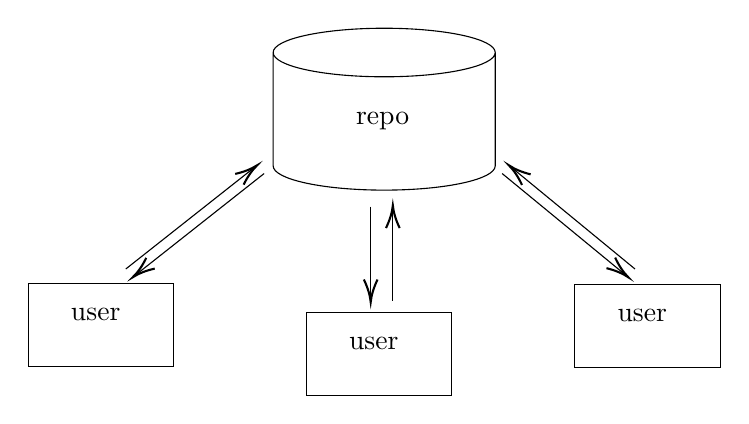
\begin{tikzpicture}[x=0.75pt,y=0.75pt,yscale=-1,xscale=1]
%uncomment if require: \path (0,300); %set diagram left start at 0, and has height of 300

%Shape: Can [id:dp2786160443943346] 
\draw   (409.67,73.03) -- (409.67,127.63) .. controls (409.67,134.1) and (385.71,139.33) .. (356.17,139.33) .. controls (326.62,139.33) and (302.67,134.1) .. (302.67,127.63) -- (302.67,73.03) .. controls (302.67,66.57) and (326.62,61.33) .. (356.17,61.33) .. controls (385.71,61.33) and (409.67,66.57) .. (409.67,73.03) .. controls (409.67,79.5) and (385.71,84.73) .. (356.17,84.73) .. controls (326.62,84.73) and (302.67,79.5) .. (302.67,73.03) ;
%Shape: Rectangle [id:dp5804880297256121] 
\draw   (184.67,184.33) -- (254.67,184.33) -- (254.67,224.33) -- (184.67,224.33) -- cycle ;
%Shape: Rectangle [id:dp45826603462909665] 
\draw   (318.67,198.33) -- (388.67,198.33) -- (388.67,238.33) -- (318.67,238.33) -- cycle ;
%Shape: Rectangle [id:dp027544595740327416] 
\draw   (448,185) -- (518,185) -- (518,225) -- (448,225) -- cycle ;
%Straight Lines [id:da9610493616903942] 
\draw    (231.67,177.33) -- (293.43,128.57) ;
\draw [shift={(295,127.33)}, rotate = 501.71] [color={rgb, 255:red, 0; green, 0; blue, 0 }  ][line width=0.75]    (10.93,-3.29) .. controls (6.95,-1.4) and (3.31,-0.3) .. (0,0) .. controls (3.31,0.3) and (6.95,1.4) .. (10.93,3.29)   ;
%Straight Lines [id:da5107911626847681] 
\draw    (298.33,131.33) -- (236.57,180.09) ;
\draw [shift={(235,181.33)}, rotate = 321.71000000000004] [color={rgb, 255:red, 0; green, 0; blue, 0 }  ][line width=0.75]    (10.93,-3.29) .. controls (6.95,-1.4) and (3.31,-0.3) .. (0,0) .. controls (3.31,0.3) and (6.95,1.4) .. (10.93,3.29)   ;
%Straight Lines [id:da17177392489774002] 
\draw    (477,177.33) -- (417.74,128.6) ;
\draw [shift={(416.2,127.33)}, rotate = 399.43] [color={rgb, 255:red, 0; green, 0; blue, 0 }  ][line width=0.75]    (10.93,-3.29) .. controls (6.95,-1.4) and (3.31,-0.3) .. (0,0) .. controls (3.31,0.3) and (6.95,1.4) .. (10.93,3.29)   ;
%Straight Lines [id:da26959159300812263] 
\draw    (413,131.33) -- (472.26,180.06) ;
\draw [shift={(473.8,181.33)}, rotate = 219.43] [color={rgb, 255:red, 0; green, 0; blue, 0 }  ][line width=0.75]    (10.93,-3.29) .. controls (6.95,-1.4) and (3.31,-0.3) .. (0,0) .. controls (3.31,0.3) and (6.95,1.4) .. (10.93,3.29)   ;
%Straight Lines [id:da3848074645987064] 
\draw    (349.67,147.33) -- (349.67,191.33) ;
\draw [shift={(349.67,193.33)}, rotate = 270] [color={rgb, 255:red, 0; green, 0; blue, 0 }  ][line width=0.75]    (10.93,-3.29) .. controls (6.95,-1.4) and (3.31,-0.3) .. (0,0) .. controls (3.31,0.3) and (6.95,1.4) .. (10.93,3.29)   ;
%Straight Lines [id:da9001312207066434] 
\draw    (360.33,192.67) -- (360.33,148.67) ;
\draw [shift={(360.33,146.67)}, rotate = 450] [color={rgb, 255:red, 0; green, 0; blue, 0 }  ][line width=0.75]    (10.93,-3.29) .. controls (6.95,-1.4) and (3.31,-0.3) .. (0,0) .. controls (3.31,0.3) and (6.95,1.4) .. (10.93,3.29)   ;

% Text Node
\draw (341.33,100.67) node [anchor=north west][inner sep=0.75pt]   [align=left] {repo};
% Text Node
\draw (204,195) node [anchor=north west][inner sep=0.75pt]   [align=left] {user};
% Text Node
\draw (338,209) node [anchor=north west][inner sep=0.75pt]   [align=left] {user};
% Text Node
\draw (467.33,195.67) node [anchor=north west][inner sep=0.75pt]   [align=left] {user};


\end{tikzpicture}


}

\hfill \break In this case, there's a singular centralized codebase that users will all be contributing to at the same time.
\end{myproof}

\subsection{Distributed VCS}

Distributed VCS has no central repository, and every repository has their own commits and history. Examples of this would be \textbf{Git} and \textbf{Mercurial}.\\

\begin{tcolorbox}[title=Aside: \texttt{Git}'s popularity,colframe=black,colback=white,arc=0pt,fonttitle=\bfseries]
\texttt{Git} is currently the most widely used code management tool (VCS). The next two in line are \texttt{SVN} and \texttt{Mercurial}.
\end{tcolorbox}

\hfill \break \texttt{Git} is also more efficient and secure than \texttt{SVN}, but a lot of old legacy codebases and companies still make use of \texttt{SVN}. For that reason, it may be good to pick up some of the basics of \texttt{SVN} so I'm not totally unfamiliar, but \texttt{Git} generally seems to be preferable.

\subsection{Branching}

\texttt{Git} also allows for branches. \textbf{Merging} also ties in closely with branching on git, and has a lot more sophistication in \texttt{Git}.

\subsubsection{When Should I Branch?}

Anything in the master branch is considered to be deployable. If you're adding a new feature, working on an experiment, or trying to implement a new fix, make a branch. You can always merge it back to master once it's considered 'deployable' again.

\subsection{Git Basics}

As far as \texttt{git} is concerned, a file has 4 states:

\begin{itemize}
	\item \textbf{Modified} $\rightarrow$ File has been changed, but those changes have not been committed
	\item \textbf{Staged} $\rightarrow$ Marked to go to next commit snapshot
	\item \textbf{Committed} $\rightarrow$ Safely stored in local database as part of a 'commit'
	\item \textbf{Untracked} $\rightarrow$ News added or removed files
\end{itemize}

This idea can be complemented by a visual guide, where you can see the three main 'places' that a file can be within the \texttt{git} system.\\

{
\centering



\tikzset{every picture/.style={line width=0.75pt}} %set default line width to 0.75pt        

\begin{tikzpicture}[x=0.75pt,y=0.75pt,yscale=-1,xscale=1]
%uncomment if require: \path (0,300); %set diagram left start at 0, and has height of 300

%Shape: Rectangle [id:dp03360737972469485] 
\draw   (87.67,2) -- (235,2) -- (235,42) -- (87.67,42) -- cycle ;
%Shape: Rectangle [id:dp33101061268187126] 
\draw   (269,3.33) -- (416.33,3.33) -- (416.33,43.33) -- (269,43.33) -- cycle ;
%Shape: Rectangle [id:dp2846424801765658] 
\draw   (467.67,3.33) -- (615,3.33) -- (615,43.33) -- (467.67,43.33) -- cycle ;
%Straight Lines [id:da9065613336807579] 
\draw    (160,42) -- (160,291.33) ;
%Straight Lines [id:da2956282330861755] 
\draw    (341.67,42) -- (341.67,291.33) ;
%Straight Lines [id:da16834279927637852] 
\draw    (540.67,42) -- (540.67,291.33) ;
%Straight Lines [id:da5787373144011785] 
\draw [color={rgb, 255:red, 255; green, 0; blue, 0 }  ,draw opacity=1 ]   (540.67,70.5) -- (162,70.5) ;
\draw [shift={(160,70.5)}, rotate = 360] [color={rgb, 255:red, 255; green, 0; blue, 0 }  ,draw opacity=1 ][line width=0.75]    (10.93,-3.29) .. controls (6.95,-1.4) and (3.31,-0.3) .. (0,0) .. controls (3.31,0.3) and (6.95,1.4) .. (10.93,3.29)   ;
%Straight Lines [id:da4994076538949177] 
\draw [color={rgb, 255:red, 74; green, 144; blue, 226 }  ,draw opacity=1 ]   (160,146) -- (339.67,146) ;
\draw [shift={(341.67,146)}, rotate = 180] [color={rgb, 255:red, 74; green, 144; blue, 226 }  ,draw opacity=1 ][line width=0.75]    (10.93,-3.29) .. controls (6.95,-1.4) and (3.31,-0.3) .. (0,0) .. controls (3.31,0.3) and (6.95,1.4) .. (10.93,3.29)   ;
%Straight Lines [id:da45013717398282227] 
\draw [color={rgb, 255:red, 65; green, 117; blue, 5 }  ,draw opacity=1 ]   (341.67,221.67) -- (538.67,221.67) ;
\draw [shift={(540.67,221.67)}, rotate = 180] [color={rgb, 255:red, 65; green, 117; blue, 5 }  ,draw opacity=1 ][line width=0.75]    (10.93,-3.29) .. controls (6.95,-1.4) and (3.31,-0.3) .. (0,0) .. controls (3.31,0.3) and (6.95,1.4) .. (10.93,3.29)   ;

% Text Node
\draw (102.5,12.67) node [anchor=north west][inner sep=0.75pt]   [align=left] {working directory};
% Text Node
\draw (299.17,12.67) node [anchor=north west][inner sep=0.75pt]   [align=left] {staging area};
% Text Node
\draw (496.67,12.67) node [anchor=north west][inner sep=0.75pt]   [align=left] {git repository};
% Text Node
\draw (213.33,74.5) node [anchor=north west][inner sep=0.75pt]   [align=left] {\textcolor[rgb]{1,0,0}{checkout}};
% Text Node
\draw (188.67,150) node [anchor=north west][inner sep=0.75pt]   [align=left] {\textcolor[rgb]{0.29,0.56,0.89}{stage ({\fontfamily{pcr}\selectfont git add})}};
% Text Node
\draw (414.67,225.67) node [anchor=north west][inner sep=0.75pt]   [align=left] {\textcolor[rgb]{0.25,0.46,0.02}{commit}};


\end{tikzpicture}


}

\subsection{Online Hosting}

\textbf{Github}, \textbf{Bitbucket}, and \textbf{Gitlab} are all popular sources that will host your git repositories. Think of this as just another place for your git stuff to exist, except whenever you want to update the main online repository, perform a \texttt{git push}.\\

It's sort of like a hybrid of a centralized and distributed VCS. According to a website online, "GitHub and similar services bring all of the benefits of a decentralized VCS to a centralized service."

\section{Lecture 8}

\subsection{Missing Data}

Missing data is information that we want to know, but don't know. It can come in many forms. Here are some examples.

\begin{itemize}
	\item People omitting answers on surveys
	\item Inaccurate measurements that we need to discard- we're mainly talking about easily detectable outliers here
	\item Canceled trials of an experiment
\end{itemize}

\hfill \break To do something about this, however, we need to figure out the following.

\begin{itemize}
	\item What contributes to the \textit{probability} of a data point being absent?
	\item Can this missing data be interpolated using the data we already have? Or not?
\end{itemize}

\subsubsection{Just Deleting It}

The easiest way to deal with this is just to delete all the tuples with any missing values, so we don't have any 'incomplete observations'. All we have to do in this case is just use \texttt{df.dropna()} to trop the appropriate row.\\

Be warned that a loss of a sample could lead to a variance greater than what's reflected by the size of our data. This could cause bias. Overall, despite this being the easiest way to get rid of 'problem' data, we should avoid doing this if we can, and intelligently account for it being missing if possible.

Obviously, if we want to remain the most accurate that we can possibly be, the goal is not to throw in the towel and just toss out missing data right off the bat.

\subsection{Types of Missing Data}

Let's start by classifying missing data into a variety of different types. Missing data can fall into one of three categories. They also have commonly used abbreviations, included here.

\begin{itemize}
	\item Missing Completely at Random (\textbf{MCAR})
	\item Missing at Random (\textbf{MAR})
	\item Missing Not at Random (\textbf{MNAR})
\end{itemize}

\subsubsection{Missing Completely At Random}

Missing completely at random means exactly what it says- the data that has gone missing has gone missing completely and entirely at random- there is no rhyme or reason behind what's gone and why it went.\\

\begin{myproof}
\textbf{Example of MCAR:} Imagine you are doing an experiment on plants grown in pots, when you have a nervous breakdown and destroy some of the pots. You didn't have any bias in how you picked the pots to break, so this data is now \textbf{MCAR}.
\end{myproof}

\hfill \break However, this just isn't realistic. Data is usually missing for a reason. For example, if you're standing outside CSIC polling people for a survey and you suddenly ask for their grades, students who are failing may be less likely to reveal their grades than students who are doing well.

\subsubsection{Missing At Random}

For data that is missing at random, the probability of the missing data is dependent on the observed data, but not the unobserved data.\\

There is a \textbf{probabilistic mechanism} associated with whether the data is missing, and that mechanism takes the observed data as input.\\

\begin{myproof}
\textbf{Example:} If a child does not attend an educational assessment because the child is (genuinely) ill, this might be predictable from other data we have about the child's health, but it would not be related to what we would have measured had the child not been ill.\\\\ Since we could predict the "missing-ness" of the student's score from the student's health, this is considered \textbf{Missing At Random}. \textit{(Taken from Martin Bland's textbook: An Introduction to Medical Statistics, Fourth Edition)}
\end{myproof}

\hfill \break We can model a parameter's "missing-ness" on other properties of the data we have already.

\subsubsection{Missing Not At Random}

The "missing-ness" of a variable has something to do with the variable itself.

\begin{myproof}
\textbf{Example:} If men failed to fill out a survey because of their level of depression, their depression affects the measurement that is being taken about their depression, making this data \textbf{Missing Not at Random}.
\end{myproof}

\subsection{Line of Best Fit}

In order to aid in this, let's again revisit the idea of a 'line of best fit' from statistics. Here's a quick review.\\

\begin{tcolorbox}[title=Definition:,colframe=red!75!black,colback=red!5!white,arc=0pt,fonttitle=\bfseries]
\textbf{Line of Best Fit} $\rightarrow$ When the difference between the true y-values and the line that you're using the estimate y-values is minimized.
\end{tcolorbox}

\hfill \break This is accomplished by using the least squares method. Below is a visualization of the process. Given the following plotted points (light green), we're looking to create the line of best fit (blue).\\

{
\centering



\tikzset{every picture/.style={line width=0.75pt}} %set default line width to 0.75pt        

\begin{tikzpicture}[x=0.75pt,y=0.75pt,yscale=-1,xscale=1]
%uncomment if require: \path (0,300); %set diagram left start at 0, and has height of 300

%Straight Lines [id:da7643777205506523] 
\draw [color={rgb, 255:red, 74; green, 144; blue, 226 }  ,draw opacity=1 ]   (65,288) -- (638.44,93.97) ;
\draw [shift={(640.33,93.33)}, rotate = 521.31] [color={rgb, 255:red, 74; green, 144; blue, 226 }  ,draw opacity=1 ][line width=0.75]    (10.93,-3.29) .. controls (6.95,-1.4) and (3.31,-0.3) .. (0,0) .. controls (3.31,0.3) and (6.95,1.4) .. (10.93,3.29)   ;
%Shape: Rectangle [id:dp6573658715334976] 
\draw   (65,8.67) -- (640.33,8.67) -- (640.33,288) -- (65,288) -- cycle ;
%Shape: Circle [id:dp030383011435651586] 
\draw  [fill={rgb, 255:red, 184; green, 233; blue, 134 }  ,fill opacity=1 ] (148.63,189.13) .. controls (148.63,187.11) and (150.27,185.47) .. (152.3,185.47) .. controls (154.33,185.47) and (155.97,187.11) .. (155.97,189.13) .. controls (155.97,191.16) and (154.33,192.8) .. (152.3,192.8) .. controls (150.27,192.8) and (148.63,191.16) .. (148.63,189.13) -- cycle ;
%Shape: Circle [id:dp39783578450486057] 
\draw  [fill={rgb, 255:red, 184; green, 233; blue, 134 }  ,fill opacity=1 ] (254.33,119.93) .. controls (254.33,117.91) and (255.97,116.27) .. (258,116.27) .. controls (260.03,116.27) and (261.67,117.91) .. (261.67,119.93) .. controls (261.67,121.96) and (260.03,123.6) .. (258,123.6) .. controls (255.97,123.6) and (254.33,121.96) .. (254.33,119.93) -- cycle ;
%Straight Lines [id:da026963523494234698] 
\draw [color={rgb, 255:red, 144; green, 19; blue, 254 }  ,draw opacity=1 ]   (152.43,193.6) -- (152.3,257.2) ;
%Straight Lines [id:da6336444278407171] 
\draw [color={rgb, 255:red, 144; green, 19; blue, 254 }  ,draw opacity=1 ]   (258,123.6) -- (258,223.2) ;
%Shape: Circle [id:dp12766640087215864] 
\draw  [fill={rgb, 255:red, 184; green, 233; blue, 134 }  ,fill opacity=1 ] (431.73,217.93) .. controls (431.73,215.91) and (433.37,214.27) .. (435.4,214.27) .. controls (437.43,214.27) and (439.07,215.91) .. (439.07,217.93) .. controls (439.07,219.96) and (437.43,221.6) .. (435.4,221.6) .. controls (433.37,221.6) and (431.73,219.96) .. (431.73,217.93) -- cycle ;
%Shape: Circle [id:dp7005961980277177] 
\draw  [fill={rgb, 255:red, 184; green, 233; blue, 134 }  ,fill opacity=1 ] (576.33,156.33) .. controls (576.33,154.31) and (577.97,152.67) .. (580,152.67) .. controls (582.03,152.67) and (583.67,154.31) .. (583.67,156.33) .. controls (583.67,158.36) and (582.03,160) .. (580,160) .. controls (577.97,160) and (576.33,158.36) .. (576.33,156.33) -- cycle ;
%Straight Lines [id:da8064600665611591] 
\draw [color={rgb, 255:red, 144; green, 19; blue, 254 }  ,draw opacity=1 ]   (435.4,163.2) -- (435.4,214.27) ;
%Straight Lines [id:da09925340912653924] 
\draw [color={rgb, 255:red, 144; green, 19; blue, 254 }  ,draw opacity=1 ]   (580,152.67) -- (580,113.6) ;

% Text Node
\draw (130.3,212.8) node [anchor=north west][inner sep=0.75pt]   [align=left] {\textcolor[rgb]{0.56,0.07,1}{E$\displaystyle _{1}$}};
% Text Node
\draw (236,154.4) node [anchor=north west][inner sep=0.75pt]   [align=left] {\textcolor[rgb]{0.56,0.07,1}{E}\textcolor[rgb]{0.56,0.07,1}{$\displaystyle _{2}$}};
% Text Node
\draw (413.4,182.8) node [anchor=north west][inner sep=0.75pt]   [align=left] {\textcolor[rgb]{0.56,0.07,1}{E}\textcolor[rgb]{0.56,0.07,1}{$\displaystyle _{3}$}};
% Text Node
\draw (558,126) node [anchor=north west][inner sep=0.75pt]   [align=left] {\textcolor[rgb]{0.56,0.07,1}{E}\textcolor[rgb]{0.56,0.07,1}{$\displaystyle _{4}$}};
% Text Node
\draw (308.01,184.87) node [anchor=north west][inner sep=0.75pt]  [rotate=-341] [align=left] {\textcolor[rgb]{0.29,0.56,0.89}{Line of Best Fit}};


\end{tikzpicture}


}

\hfill \break Here, using the least squares method, we try to minimize the equation yielded by the following summation. 

$$ \sum_{i=1}^{n} {(E_i)^2} = (E_1)^2 + (E_2)^2 + ... (E_n)^2$$












\section{Footnotes}

Taken by Akilesh Praveen.

\end{document}
